% ============================================================
%  MAIN.TEX — Central assembly file
% ============================================================

\documentclass[
  12pt,
  a4paper,
  twoside,
  openany,
  final
]{report}

% ── 1. LOAD ALL PACKAGES & GLOBAL CONFIGURATION ─────────────
% ============================================================
%  styles/packages.tex
%  Central package registry — all \usepackage declarations
%  Organised by category with inline rationale
% ============================================================

% ── ENGINE & ENCODING ────────────────────────────────────────
\usepackage{iftex}
\ifLuaTeX
  \usepackage{fontspec}           % OpenType font loading (LuaLaTeX)
  \usepackage{luacode}
\else
  \usepackage[T1]{fontenc}
  \usepackage[utf8]{inputenc}
\fi

% ── LANGUAGE & LOCALISATION ──────────────────────────────────
\usepackage[
  main=english,
  french,
  arabic
]{babel}                          % Multi-language support
\usepackage{csquotes}             % Context-sensitive quotes (required by biblatex)

% ── PAGE LAYOUT ──────────────────────────────────────────────
\usepackage[
  a4paper,
  top=2.5cm, bottom=2.5cm,
  left=2.5cm, right=2.5cm,       % Symmetric margins for uniform consistency
  headsep=1cm,
  headheight=15pt,
  footskip=1.5cm
]{geometry}
\usepackage{emptypage}            % Suppress headers on blank pages
\usepackage{pdflscape}            % Landscape pages inside portrait doc
\usepackage{rotating}             % Rotate floats/text

% ── TYPOGRAPHY ───────────────────────────────────────────────
\usepackage{microtype}            % Micro-typography (protrusion, expansion)
\usepackage{setspace}             % Line spacing control
\usepackage{ragged2e}             % Improved justification
\usepackage{soul}                 % Underlining, striking, highlighting
\usepackage{ulem}                 % Strikethrough etc. (normalem keeps \emph)
\normalem

% ── HEADERS & FOOTERS ────────────────────────────────────────
\usepackage{fancyhdr}             % Custom headers and footers
\usepackage{lastpage}             % \pageref{LastPage} for "page X of Y"

% ── COLORS ───────────────────────────────────────────────────
\usepackage[dvipsnames, svgnames, x11names, table]{xcolor}

% ── MATHEMATICS ──────────────────────────────────────────────
\usepackage{amsmath, amssymb, amsthm}
\usepackage{mathtools}            % Extends amsmath
\usepackage{bm}                   % Bold math symbols
\usepackage{siunitx}              % SI units: \SI{9.8}{\meter\per\second\squared}

% ── FIGURES & GRAPHICS ───────────────────────────────────────
\usepackage{graphicx}             % \includegraphics
\usepackage{float}                % [H] placement specifier
\usepackage{wrapfig}              % Text-wrapped figures
\usepackage{subcaption}           % Sub-figures and sub-tables
\usepackage{caption}              % Custom caption formatting
\usepackage{tikz}                 % Programmatic diagrams
\usetikzlibrary{
  shapes, arrows.meta, positioning,
  calc, decorations.pathmorphing,
  backgrounds, fit, matrix
}
\usepackage{pgfplots}             % Data plots
\pgfplotsset{compat=1.18}
\usepackage{pgf-umlsd}            % UML sequence diagrams
\usepackage{forest}               % Tree structures

% ── CUSTOM FLOAT: DIAGRAMS ───────────────────────────────────
\usepackage{newfloat}
\DeclareFloatingEnvironment[
  fileext=lod,
  listname={List of Diagrams},
  name=Diagram,
  placement=tbhp,
  within=chapter
]{diagram}

% ── TABLES ───────────────────────────────────────────────────
\usepackage{booktabs}             % Professional table rules
\usepackage{tabularx}             % Tables with auto-width columns
\usepackage{longtable}            % Multi-page tables
\usepackage{multirow}             % Cells spanning multiple rows
\usepackage{makecell}             % Line breaks inside cells
\usepackage{array}                % Extended column specifications
\usepackage{colortbl}             % Colored table cells
\usepackage{hhline}               % Better double hlines in tables

% ── LISTS ────────────────────────────────────────────────────
\usepackage{enumitem}             % Control over list spacing & labels

% ── CODE LISTINGS ────────────────────────────────────────────
\usepackage{listings}             % Verbatim code with highlighting
\usepackage{minted}               % Syntax highlighting via Pygments
                                  % Requires --shell-escape flag

% ── ALGORITHMS ───────────────────────────────────────────────
\usepackage[ruled, vlined, linesnumbered]{algorithm2e}

% ── BIBLIOGRAPHY ─────────────────────────────────────────────
\usepackage[
  backend=biber,
  style=ieee,                     % IEEE citation style
  sorting=nyt,
  maxbibnames=99,
  giveninits=true,
  isbn=false,
  url=true,
  doi=true
]{biblatex}

% ── GLOSSARY & ACRONYMS ──────────────────────────────────────
\usepackage[
  acronym,
  toc,
  nonumberlist,
  nogroupskip,
  automake
]{glossaries-extra}

% ── INDEX ────────────────────────────────────────────────────
\usepackage{imakeidx}
\makeindex[columns=2, title=Index, intoc]

% ── CROSS-REFERENCES & LINKS ─────────────────────────────────
% hyperref must be loaded LAST (with few exceptions)
\usepackage{varioref}             % Smart page references: "on page 12"

% ── MISCELLANEOUS UTILITIES ──────────────────────────────────
\usepackage{lipsum}               % Placeholder text (remove in production)
\usepackage{comment}              % Multi-line comment blocks
\usepackage{pdfpages}             % Insert external PDF pages
\usepackage{epigraph}             % Chapter epigraphs/quotes
\usepackage{tcolorbox}            % Colored info/warning boxes
\tcbuselibrary{skins, breakable, theorems, listings}
\usepackage{mdframed}             % Framed environments
\usepackage{todonotes}            % \todo{} margin notes (disable in final)
\usepackage{xspace}               % Intelligent spacing after macros
\usepackage{etoolbox}             % Toolbox for LaTeX programmers
\usepackage{xparse}               % Advanced command definitions
\usepackage{calc}                 % Arithmetic in length expressions
\usepackage{eso-pic}              % Absolute positioning on pages (cover)
\usepackage{tikzpagenodes}        % TikZ page node access
\usepackage{qrcode}               % QR codes: \qrcode{https://...}
\usepackage{fontawesome5}          % Icons: \faExclamationTriangle etc.

% ============================================================
%  styles/colors.tex
%  Palette : #232527 (primaire) · #CF0A2C (secondaire)
% ============================================================
 
% ── COULEURS PRINCIPALES ─────────────────────────────────────
\definecolor{PrimaryDark}    {HTML}{232527}   % Presque noir — couleur principale
\definecolor{SecondaryRed}   {HTML}{CF0A2C}   % Rouge vif   — couleur secondaire
 
% ── COULEURS SÉMANTIQUES ─────────────────────────────────────
\definecolor{ChapterColor}   {HTML}{232527}
\definecolor{SectionColor}   {HTML}{232527}
\definecolor{LinkColor}      {HTML}{CF0A2C}
\definecolor{CiteColor}      {HTML}{232527}
\definecolor{UrlColor}       {HTML}{CF0A2C}
 
% ── INTERFACE / BOÎTES ───────────────────────────────────────
\definecolor{LightGrayBg}    {HTML}{F5F5F5}
\definecolor{MidGray}        {HTML}{888888}
\definecolor{DarkGray}       {HTML}{444444}
\definecolor{BodyText}       {HTML}{232527}
\definecolor{RuleColor}      {HTML}{232527}
 
% ── TABLEAUX ─────────────────────────────────────────────────
\definecolor{TableHeaderBg}  {HTML}{E9ECEF}   % Light professional gray
\definecolor{TableRowOdd}    {HTML}{F8F9FA}   % Very subtle alternating row
\definecolor{TableRowEven}   {HTML}{FFFFFF}
\definecolor{TableBorder}    {HTML}{DEE2E6}
 
% ── CODE ─────────────────────────────────────────────────────
\definecolor{CodeBg}         {HTML}{F7F7F7}
\definecolor{CodeBorder}     {HTML}{E0E0E0}
\definecolor{CodeKeyword}    {HTML}{CF0A2C}
\definecolor{CodeComment}    {HTML}{777777}
\definecolor{CodeString}     {HTML}{232527}
\definecolor{CodeNumber}     {HTML}{CF0A2C}
 
% ── BOÎTES CALLOUT ───────────────────────────────────────────
\definecolor{InfoBg}         {HTML}{F5F5F5}
\definecolor{InfoBorder}     {HTML}{232527}
\definecolor{WarnBg}         {HTML}{FFF5F5}
\definecolor{WarnBorder}     {HTML}{CF0A2C}
 
% ── PAGE DE GARDE ────────────────────────────────────────────
\definecolor{CoverTopRule}   {HTML}{CF0A2C}
\definecolor{CoverBotRule}   {HTML}{CF0A2C}
\definecolor{CoverDivider}   {HTML}{232527}

% ── COMPATIBILITY ALIASES (Prevent breaks in legacy TikZ/diagrams) ──
\colorlet{PrimaryBlue}{PrimaryDark}
\colorlet{SecondaryBlue}{SecondaryRed}
\colorlet{AccentGold}{SecondaryRed}
\colorlet{AccentGreen}{PrimaryDark}
\colorlet{AccentRed}{SecondaryRed}

\colorlet{InfoBlue}{InfoBg}
\colorlet{InfoBlueBorder}{InfoBorder}
\colorlet{WarnAmber}{WarnBg}
\colorlet{WarnAmberBorder}{WarnBorder}
\colorlet{DangerRed}{WarnBg}
\colorlet{DangerRedBorder}{WarnBorder}
\colorlet{SuccessGreen}{InfoBg}
\colorlet{SuccessGreenBorder}{InfoBorder}
\colorlet{TipPurple}{InfoBg}
\colorlet{TipPurpleBorder}{InfoBorder}

\colorlet{LightGray}{LightGrayBg}
\colorlet{BodyText}{BodyText}

% ============================================================
%  styles/fonts.tex — version universelle (LuaLaTeX + pdfLaTeX)
% ============================================================

\ifLuaTeX
  \usepackage{fontspec}
  \setmainfont{Latin Modern Roman}
  \setsansfont{Latin Modern Sans}
  \setmonofont{Consolas}[Scale=0.9] % Consolas supports box drawing characters better
  \babelfont[arabic]{rm}[Renderer=HarfBuzz]{Arial} % Improved Arabic rendering
  \babelfont[arabic]{sf}[Renderer=HarfBuzz]{Arial}
  \babelfont[arabic]{tt}[Renderer=HarfBuzz]{Arial}
\else
  \usepackage{lmodern}
\fi

% \HeadingFont — défini une seule fois, compatible les deux moteurs
\newcommand{\HeadingFont}{\sffamily}

% ── INTERLIGNE ───────────────────────────────────────────────
\setstretch{1.25}

% ── PARAGRAPHES ──────────────────────────────────────────────
\setlength{\parindent}{0pt}
\setlength{\parskip}{6pt plus 2pt minus 1pt}

% ============================================================
%  styles/layout.tex
%  Page geometry, chapter/section styling, headers & footers
% ============================================================

% ── CHAPTER STYLE (titlesec) ─────────────────────────────────
\usepackage{titlesec}
\usepackage{titletoc}

% Chapter title format — full-width colored bar
\titleformat{\chapter}[display]
  {\normalfont\huge\bfseries\color{ChapterColor}\HeadingFont}  % format
  {%
    \vspace{-20pt}%
    \colorbox{ChapterColor}{%
      \parbox[c][1.8cm][c]{\textwidth}{%
        \centering\color{white}\fontsize{14}{16}\selectfont
        \MakeUppercase{\chaptertitlename}\hspace{10pt}%
        \fontsize{40}{44}\selectfont\thechapter
      }%
    }%
  }
  {0pt}                          % separation between label and title
  {\vspace{10pt}\raggedright}    % before-code
  [\vspace{8pt}\textcolor{AccentGold}{\hrule height 2pt}\vspace{12pt}]

% Section format
\titleformat{\section}
  {\normalfont\Large\bfseries\color{SectionColor}\HeadingFont}
  {\thesection}{1em}{}
  [\vspace{-4pt}\textcolor{SectionColor!40}{\hrule height 0.5pt}]

% Subsection format
\titleformat{\subsection}
  {\normalfont\large\bfseries\color{SectionColor!80}\HeadingFont}
  {\thesubsection}{1em}{}

% Subsubsection format
\titleformat{\subsubsection}
  {\normalfont\normalsize\bfseries\itshape\color{DarkGray}\HeadingFont}
  {\thesubsubsection}{1em}{}

% Spacing around headings
\titlespacing*{\chapter}     {0pt}{0pt}{30pt}
\titlespacing*{\section}     {0pt}{18pt}{8pt}
\titlespacing*{\subsection}  {0pt}{14pt}{6pt}
\titlespacing*{\subsubsection}{0pt}{12pt}{4pt}

% ── CAPTION STYLE ────────────────────────────────────────────
\captionsetup{
  font       = {small, it},
  labelfont  = {bf, color=PrimaryBlue},
  labelsep   = period,
  justification = centering,
  skip       = 8pt
}
\captionsetup[table]{
  position   = above,
  skip       = 4pt
}

% ── HEADER & FOOTER (fancyhdr) ───────────────────────────────
\pagestyle{fancy}
\fancyhf{}  % clear all

% Two-sided layout:
%   Even pages  (left)  → chapter name on outer, page on inner
%   Odd  pages  (right) → section name on inner, page on outer
\fancyhead[LE]{%
  \small\color{MidGray}\textit{\nouppercase{\leftmark}}%
}
\fancyhead[RO]{%
  \small\color{MidGray}\textit{\nouppercase{\rightmark}}%
}
\fancyfoot[LE,RO]{%
  \small\color{MidGray}\thepage\ /\ \pageref{LastPage}%
}
\fancyfoot[LO,RE]{%
  \small\color{MidGray}\textit{\ReportTitleShort}%
}

% Header/footer rules
\renewcommand{\headrulewidth}{0.4pt}
\renewcommand{\footrulewidth}{0.4pt}
\renewcommand{\headrule}{%
  {\color{PrimaryBlue}\hrule width\headwidth height\headrulewidth}%
}
\renewcommand{\footrule}{%
  {\color{AccentGold}\hrule width\headwidth height\footrulewidth}%
}

% Plain style for chapter opening pages
\fancypagestyle{plain}{
  \fancyhf{}
  \fancyfoot[C]{\small\color{MidGray}\thepage}
  \renewcommand{\headrulewidth}{0pt}
  \renewcommand{\footrulewidth}{0.4pt}
  \renewcommand{\footrule}{%
    {\color{AccentGold}\hrule width\headwidth height\footrulewidth}%
  }
}

% Cover page style — completely empty
\fancypagestyle{cover}{
  \fancyhf{}
  \renewcommand{\headrulewidth}{0pt}
  \renewcommand{\footrulewidth}{0pt}
}

% ── LIST STYLES ──────────────────────────────────────────────
\setlist{
  topsep    = 4pt,
  itemsep   = 2pt,
  parsep    = 0pt,
  leftmargin= 1.5em
}
\setlist[itemize,1]{label=\textcolor{PrimaryBlue}{\textbullet}}
\setlist[itemize,2]{label=\textcolor{SecondaryBlue}{\textendash}}
\setlist[enumerate,1]{label=\textcolor{PrimaryBlue}{\arabic*.}}

% ── FLOAT SETTINGS ───────────────────────────────────────────
\setcounter{topnumber}    {3}
\setcounter{bottomnumber} {2}
\setcounter{totalnumber}  {5}
\renewcommand{\topfraction}    {0.85}
\renewcommand{\bottomfraction} {0.60}
\renewcommand{\textfraction}   {0.10}
\renewcommand{\floatpagefraction}{0.75}

% ── DEPTH SETTINGS ───────────────────────────────────────────
\setcounter{tocdepth}    {3}   % TOC shows up to subsubsection
\setcounter{secnumdepth} {3}   % Numbering up to subsubsection

% ── DOCUMENT MATTERS (for report class) ──────────────────────
\newcommand{\frontmatter}{%
  \cleardoublepage
  \pagenumbering{roman}
  \assignpagestyle{\chapter}{empty}
}

\newcommand{\mainmatter}{%
  \cleardoublepage
  \pagenumbering{arabic}
  \assignpagestyle{\chapter}{plain}
  \raggedbottom
  \emergencystretch 3em
}

\newcommand{\backmatter}{%
  \cleardoublepage
}

% ============================================================
%  styles/macros.tex
%  Custom commands, environments, and reusable building blocks
% ============================================================

% ── TEXT UTILITIES ───────────────────────────────────────────

% Highlight a term on first use
\newcommand{\term}[1]{\textbf{\textit{#1}}}

% Small caps abbreviation
\newcommand{\abbr}[1]{\textsc{\lowercase{#1}}}

% Emphasis that also adds to index
\newcommand{\idxterm}[1]{\textbf{#1}\index{#1}}

% Inline code snippet (allows line breaks)
\newcommand{\code}[1]{\texttt{\small\textcolor{CodeKeyword}{\hyphenchar\font=`\-\relax #1}}}

% File path (allows line breaks)
\newcommand{\filepath}[1]{\texttt{\small\textit{\hyphenchar\font=`\-\relax #1}}}

% Package name
\newcommand{\pkg}[1]{\textsf{#1}}

% Versioned software reference: \software{Docker}{20.10.7}
\newcommand{\software}[2]{\textit{#1}~v#2}

% ── MATH UTILITIES ───────────────────────────────────────────

% Norm  ||x||
\newcommand{\norm}[1]{\left\lVert#1\right\rVert}

% Absolute value |x|
\newcommand{\abs}[1]{\left\lvert#1\right\rvert}

% Sets
\newcommand{\R}{\mathbb{R}}
\newcommand{\N}{\mathbb{N}}
\newcommand{\Z}{\mathbb{Z}}

% ── THEOREM ENVIRONMENTS ─────────────────────────────────────
\theoremstyle{definition}
\newtheorem{definition}{Definition}[chapter]
\newtheorem{example}{Example}[chapter]
\newtheorem{remark}{Remark}[chapter]

\theoremstyle{plain}
\newtheorem{theorem}{Theorem}[chapter]
\newtheorem{lemma}[theorem]{Lemma}
\newtheorem{proposition}[theorem]{Proposition}

% ── CALLOUT BOXES (tcolorbox) ────────────────────────────────

% \infobox{Title}{Body text}
\newcommand{\infobox}[2]{%
  \begin{tcolorbox}[
    title       = #1,
    colback     = InfoBlue,
    colframe    = InfoBlueBorder,
    coltitle    = black,
    fonttitle   = \bfseries\small,
    breakable,
    left=6pt, right=6pt, top=4pt, bottom=4pt
  ]
  \small #2
  \end{tcolorbox}%
}

% \warnbox{Title}{Body text}
\newcommand{\warnbox}[2]{%
  \begin{tcolorbox}[
    title       = {\faExclamationTriangle\hspace{4pt}#1},
    colback     = WarnAmber,
    colframe    = WarnAmberBorder,
    coltitle    = black,
    fonttitle   = \bfseries\small,
    breakable,
    left=6pt, right=6pt, top=4pt, bottom=4pt
  ]
  \small #2
  \end{tcolorbox}%
}

% \tipbox{Title}{Body text}
\newcommand{\tipbox}[2]{%
  \begin{tcolorbox}[
    title       = #1,
    colback     = TipPurple,
    colframe    = TipPurpleBorder,
    coltitle    = white,
    fonttitle   = \bfseries\small,
    breakable,
    left=6pt, right=6pt, top=4pt, bottom=4pt
  ]
  \small #2
  \end{tcolorbox}%
}

% ── CHAPTER EPIGRAPH STYLE ───────────────────────────────────
\setlength{\epigraphwidth}{0.6\textwidth}
\renewcommand{\epigraphflush}{flushright}
\renewcommand{\epigraphrule}{0.4pt}

% ── FIGURE HELPERS ───────────────────────────────────────────

% Standard figure: \fig[options]{file}{caption}{label}
% options default to width=\textwidth
\NewDocumentCommand{\fig}{ O{width=\textwidth} m m m }{%
  \begin{figure}[htbp]
    \centering
    \includegraphics[#1]{#2}
    \caption{#3}
    \label{fig:#4}
  \end{figure}%
}

% Wide figure spanning full text width
\NewDocumentCommand{\widefig}{ m m m }{%
  \begin{figure}[htbp]
    \centering
    \includegraphics[width=\linewidth]{#1}
    \caption{#2}
    \label{fig:#3}
  \end{figure}%
}

% ── TABLE HELPERS ────────────────────────────────────────────

% Set global table spacing for a modern look
\renewcommand{\arraystretch}{1.3}

% Colored header row: \tableheader{Col1 & Col2 & Col3}
\newcommand{\tableheader}[1]{%
  \rowcolor{TableHeaderBg}%
  \bfseries\color{PrimaryDark}#1%
}

% Alternating row colors environment
\newenvironment{prettytable}[1]{%
  \rowcolors{2}{TableRowOdd}{TableRowEven}%
  \begin{tabular}{#1}%
  \toprule
}{%
  \bottomrule
  \end{tabular}%
}

% ── TABULARX COLUMN TYPES ────────────────────────────────────
\newcolumntype{L}{>{\raggedright\arraybackslash}X}
\newcolumntype{C}{>{\centering\arraybackslash}X}
\newcolumntype{R}{>{\raggedleft\arraybackslash}X}
\newcolumntype{P}[1]{>{\raggedright\arraybackslash}p{#1}}

% Column type that allows breaking for code-like text in tables
\newcolumntype{K}{>{\raggedright\arraybackslash\ttfamily\small}X}


% ── REFERENCE SHORTCUTS ──────────────────────────────────────
\newcommand{\figref}[1]{\hyperref[fig:#1]{Figure~\ref*{fig:#1}}}
\newcommand{\tabref}[1]{\hyperref[tab:#1]{Table~\ref*{tab:#1}}}
\newcommand{\chapref}[1]{\hyperref[chap:#1]{Chapter~\ref*{chap:#1}}}
\newcommand{\secref}[1]{\hyperref[sec:#1]{Section~\ref*{sec:#1}}}
\newcommand{\appref}[1]{\hyperref[app:#1]{Appendix~\ref*{app:#1}}}
\newcommand{\algref}[1]{\hyperref[alg:#1]{Algorithm~\ref*{alg:#1}}}
\newcommand{\diagref}[1]{\hyperref[diag:#1]{Diagram~\ref*{diag:#1}}}
\newcommand{\lstref}[1]{\hyperref[lst:#1]{Listing~\ref*{lst:#1}}}

% ── DRAFT UTILITIES ──────────────────────────────────────────
% Comment out for final version:
% \newcommand{\draftonly}[1]{#1}          % Show in draft
% \newcommand{\draftonly}[1]{}            % Hide in final
\newcommand{\draftonly}[1]{%
  \textcolor{red}{\textit{[DRAFT: #1]}}%
}

% ── PAGE BREAK CONTROL ───────────────────────────────────────
\newcommand{\chapterbreak}{\cleardoublepage}

% ── LOGO GRID (used in sec-4-software-stack) ─────────────────

\newcommand{\logocard}[2]{%
  \begin{minipage}[c]{2.8cm}
    \centering
    \IfFileExists{images/tools/#1.png}{%
      \includegraphics[height=1.0cm, keepaspectratio]{images/tools/#1}%
    }{%
      \fcolorbox{PrimaryDark}{LightGrayBg}{%
        \parbox[c][1.0cm][c]{2.2cm}{\centering\tiny\color{MidGray}#2}%
      }%
    }\\[4pt]
    {\tiny\color{DarkGray}#2}
  \end{minipage}%
}

\newenvironment{logogrid}{%
  \vspace{6pt}%
  \begin{center}%
  \setlength{\tabcolsep}{6pt}%
}{%
  \end{center}%
  \vspace{4pt}%
}
% ============================================================
%  styles/listings.tex
%  Code listing styles for both `listings` and `minted`
% ============================================================

% ── LISTINGS PACKAGE GLOBAL DEFAULTS ────────────────────────
\lstset{
  backgroundcolor  = \color{CodeBg},
  basicstyle       = \ttfamily\small\color{BodyText},
  keywordstyle     = \color{CodeKeyword}\bfseries,
  commentstyle     = \color{CodeComment}\itshape,
  stringstyle      = \color{CodeString},
  numberstyle      = \tiny\color{MidGray},
  breakatwhitespace= false,
  breaklines       = true,
  captionpos       = b,
  frame            = single,
  framerule        = 0.4pt,
  rulecolor        = \color{CodeBorder},
  keepspaces       = true,
  numbers          = left,
  numbersep        = 10pt,
  showspaces       = false,
  showstringspaces = false,
  showtabs         = false,
  tabsize          = 2,
  xleftmargin      = 15pt,
  framexleftmargin = 15pt,
  aboveskip        = 12pt,
  belowskip        = 12pt,
  literate         = {á}{{\'a}}1 {é}{{\'e}}1 {í}{{\'i}}1
                     {ó}{{\'o}}1 {ú}{{\'u}}1
}

% Language-specific styles
\lstdefinestyle{Python}{
  language    = Python,
  morekeywords= {self, True, False, None, async, await, yield}
}

\lstdefinestyle{Java}{
  language    = Java,
  morekeywords= {var, record, sealed, permits}
}

\lstdefinestyle{JavaScript}{
  language    = Java,    % closest built-in
  morekeywords= {const, let, async, await, of, from, import, export,
                 function, class, extends, new, return, typeof,
                 undefined, null, true, false, =>}
}

\lstdefinestyle{Bash}{
  language    = bash,
  morekeywords= {docker, kubectl, git, npm, pip, make}
}

\lstdefinestyle{YAML}{
  language    = python,  % closest built-in for YAML
  morekeywords= {true, false, null},
  literate    = {:}{{{\textcolor{CodeKeyword}{:}}}}{1}
}

\lstdefinestyle{SQL}{
  language    = SQL,
  morekeywords= {CREATE, ALTER, DROP, INSERT, UPDATE, DELETE,
                 SELECT, FROM, WHERE, JOIN, INNER, OUTER,
                 LEFT, RIGHT, ON, GROUP, ORDER, BY, HAVING}
}

% ── MINTED (preferred when --shell-escape is available) ──────
% Usage: \begin{minted}[options]{language} ... \end{minted}
% Or: \mintinline{python}{for x in range(10):}
% Or: \inputminted{python}{code/example.py}

% Default minted style
\setminted{
  style        = friendly,
  bgcolor      = CodeBg,
  fontsize     = \small,
  linenos      = true,
  numbersep    = 8pt,
  frame        = lines,
  framesep     = 2mm,
  breaklines   = true,
  autogobble   = true,
  tabsize      = 2
}

% ── CUSTOM LISTINGS ENVIRONMENT ──────────────────────────────
% \begin{codebox}[Python]{My Python example}{lst:example}
% ... code ...
% \end{codebox}
\NewDocumentEnvironment{codebox}{ O{} m m }{%
  \begin{tcolorbox}[
    listing only,
    title   = \texttt{#2},
    label   = #3,
    colback = CodeBg,
    colframe= PrimaryBlue,
    coltitle= white,
    fonttitle=\bfseries\small\ttfamily,
    breakable,
    left=0pt, right=0pt, top=0pt, bottom=0pt
  ]
  \lstset{style=#1}%
}{%
  \end{tcolorbox}%
}

% ============================================================
%  styles/hyperref-setup.tex
%  PDF metadata, hyperlinks, bookmarks
%  Must be loaded AFTER most other packages
% ============================================================

\usepackage[
  unicode,
  pdfencoding  = auto,
  colorlinks   = true,
  linkcolor    = LinkColor,
  citecolor    = CiteColor,
  urlcolor     = UrlColor,
  filecolor    = LinkColor,
  menucolor    = LinkColor,
  runcolor     = LinkColor,
  bookmarks    = true,
  bookmarksopen= true,
  bookmarksnumbered = true,
  pdfstartview = FitH,
  pdfdisplaydoctitle = true,
  pdfpagelayout= TwoPageRight,
  pdfpagemode  = UseOutlines,
  breaklinks   = true,
  hidelinks    = false
]{hyperref}

\usepackage[nameinlink]{cleveref} % Must be loaded AFTER hyperref

% Populate PDF metadata from metadata.tex values
\AtBeginDocument{%
  \hypersetup{
    pdftitle    = {\PDFTitle},
    pdfauthor   = {\PDFAuthor},
    pdfsubject  = {\PDFSubject},
    pdfkeywords = {\PDFKeywords},
    pdfcreator  = {LuaLaTeX + biblatex + glossaries-extra},
    pdfproducer = {LaTeX with hyperref}
  }%
}


% ── 2. DOCUMENT METADATA ────────────────────────────────────
% ============================================================
%  styles/metadata.tex
%  Single source of truth for all document metadata.
%  Edit here — values propagate everywhere automatically.
% ============================================================

% ── INSTITUTION ──────────────────────────────────────────────
\newcommand{\UniversityName}{Hassan II University}
\newcommand{\FacultyName}{Faculty of Sciences and Technology Mohammedia}
\newcommand{\DepartmentName}{Department of Mathematics}
\newcommand{\ProgramName}{Engineering Degree — Data \& Computer Science}

% ── MINISTRY ─────────────────────────────────────────────────
\newcommand{\MinistryName}{%
  Ministry of Higher Education, \\
  Scientific Research and Innovation
}
\newcommand{\MinistryNameShort}{MESRI}

% ── HOST COMPANY (for internship reports) ────────────────────
\newcommand{\CompanyName}{Huawei Morocco}
\newcommand{\CompanyDivision}{Technologies Co. Ltd.}
\newcommand{\CompanyCity}{Casablanca, Morocco}
\newcommand{\InternshipPeriod}{April 1 -- July 31, 2026}

% ── REPORT DETAILS ───────────────────────────────────────────
\newcommand{\ReportTitle}{%
  Cross-Hardware AI Benchmarking\\
  and Deployment Optimization Across\\
  Huawei Ascend and NVIDIA CUDA Ecosystems
}
\newcommand{\ReportTitleShort}{AI Cross-Hardware Benchmarking}
\newcommand{\ReportSubtitle}{%
  End-of-Year Internship Project\\[4pt]
  \textit{In partial fulfilment of the requirements for the\\
  Engineering Diploma in Data \& Computer Science}
}
\newcommand{\ReportType}{End-of-Year Project (PFA)}
\newcommand{\AcademicYear}{2025 -- 2026}
\newcommand{\ReportDate}{June 2026}
\newcommand{\ReportLocation}{Casablanca, Morocco}

% ── AUTHOR ───────────────────────────────────────────────────
\newcommand{\AuthorFirstName}{Aya}
\newcommand{\AuthorLastName}{KIHAL}
\newcommand{\AuthorFullName}{\AuthorFirstName{} \AuthorLastName}
\newcommand{\AuthorEmail}{kihalaya00@gmail.com}
\newcommand{\StudentID}{20210512}

% ── SUPERVISORS ──────────────────────────────────────────────
\newcommand{\AcademicSupervisorName}{Pr. Karam ALLALI}
\newcommand{\AcademicSupervisorTitle}{Professor, Head of Department of Mathematics}
\newcommand{\AcademicSupervisorInst}{\FacultyName}

\newcommand{\IndustrialSupervisorName}{Mr. Zhang ZHEQIAN}
\newcommand{\IndustrialSupervisorTitle}{Data Center Solutions Department Director}
\newcommand{\IndustrialSupervisorInst}{\CompanyName}

% ── JURY MEMBERS (for thesis/defense) ────────────────────────
\newcommand{\DefenseDate}{June 18, 2026}

\newcommand{\JuryPresidentName}{Pr.K.ALLALI}
\newcommand{\JuryPresidentRole}{}
\newcommand{\JuryMemberOneName}{Pr.N.MOUSSAID}
\newcommand{\JuryMemberOneRole}{}
% Add a second examiner placeholder for layout consistency if needed
\newcommand{\JuryMemberTwoName}{} 
\newcommand{\JuryMemberTwoRole}{}

% ── LOGO PATHS ───────────────────────────────────────────────
\newcommand{\LogoUniversity}{images/logos/fstm-logo}
\newcommand{\LogoMinistry}{images/logos/logo-ministry}
\newcommand{\LogoCompany}{images/logos/Huawei-logo}

\newcommand{\LogoFaculty}{images/logos/logo-faculty}

% ── PDF METADATA (used by hyperref-setup.tex) ────────────────
\newcommand{\PDFTitle}{\ReportTitleShort}
\newcommand{\PDFAuthor}{\AuthorFullName}
\newcommand{\PDFSubject}{\ReportType\ -- \AcademicYear}
\newcommand{\PDFKeywords}{AI benchmarking, cross-hardware deployment, pipeline migration, Huawei Ascend, NVIDIA CUDA, GPU computing, NPU acceleration, CPU inference, heterogeneous computing, hardware abstraction layer, machine learning systems, large language models, model evaluation, performance benchmarking, latency measurement, throughput analysis, cost-performance optimization, model inference optimization, MLOps, model deployment pipeline, containerization, Docker, Kubernetes, cloud computing, edge AI, distributed systems, microservices architecture, workflow orchestration, FastAPI, AI infrastructure optimization, workload profiling, experimental evaluation, model selection system, intelligent recommendation engine, CANN, MindSpore, ModelArts, Huawei AI ecosystem}


% ── 3. BIBLIOGRAPHY DATABASE ────────────────────────────────
\addbibresource{bibliography/references.bib}

% ── 4. GLOSSARY / ACRONYMS DATABASE ─────────────────────────
% ============================================================
%  backmatter/acronyms.tex
%  Refined acronym database — Project Essential Terms
% ============================================================

% ── HARDWARE & ARCHITECTURE ──────────────────────────────────
\newacronym{cpu}   {CPU}   {Central Processing Unit}
\newacronym{gpu}   {GPU}   {Graphics Processing Unit}
\newacronym{npu}   {NPU}   {Neural Processing Unit}
\newacronym{tpu}   {TPU}   {Tensor Processing Unit}
\newacronym{sm}    {SM}    {Streaming Multiprocessor}
\newacronym{mac}   {MAC}   {Multiply-Accumulate}
\newacronym{hbm}   {HBM}   {High-Bandwidth Memory}
\newacronym{hbm2}  {HBM2}  {High-Bandwidth Memory Generation 2}
\newacronym{dsa}   {DSA}   {Domain-Specific Architecture}

% ── PARALLEL & ECOSYSTEMS ────────────────────────────────────
\newacronym{cuda}  {CUDA}  {Compute Unified Device Architecture}
\newacronym{cann}  {CANN}  {Compute Architecture for Neural Networks}
\newacronym{hccl}  {HCCL}  {Huawei Collective Communications Library}
\newacronym{nccl}  {NCCL}  {NVIDIA Collective Communications Library}
\newacronym{hccs}  {HCCS}  {Huawei Cache Coherence System}
\newacronym{atc}   {ATC}   {Ascend Tensor Compiler}
\newacronym{acl}   {ACL}   {Ascend Computing Language}
\newacronym{simt}  {SIMT}  {Single Instruction Multiple Thread}
\newacronym{ptx}   {PTX}   {Parallel Thread Execution}
\newacronym{mte}   {MTE}   {Memory Transfer Engine}
\newacronym{tops}  {TOPS}  {Tera Operations Per Second}
\newacronym{sct}   {SCT}   {Source Code Transformation}

% ── DEEP LEARNING & MODELS ───────────────────────────────────
\newacronym{llm}   {LLM}   {Large Language Model}
\newacronym{moe}   {MoE}   {Mixture of Experts}
\newacronym{ssm}   {SSM}   {State Space Model}
\newacronym{ffn}   {FFN}   {Feed-Forward Network}
\newacronym{sft}   {SFT}   {Supervised Fine-Tuning}
\newacronym{rl}    {RL}    {Reinforcement Learning}
\newacronym{grpo}  {GRPO}  {Group Relative Policy Optimization}
\newacronym{kv}    {KV}    {Key-Value}
\newacronym{lora}  {LoRA}  {Low-Rank Adaptation}
\newacronym{peft}  {PEFT}  {Parameter-Efficient Fine-Tuning}

% ── TOOLS & PLATFORMS ────────────────────────────────────────
\newacronym{mindie}{MindIE}{Mind Inference Engine}
\newacronym{vllm}  {vLLM}  {Virtual Large Language Model}
\newacronym{wandb} {W\&B}  {Weights \& Biases}
\newacronym{api}   {API}   {Application Programming Interface}
\newacronym{rest}  {REST}  {Representational State Transfer}
\newacronym{cli}   {CLI}   {Command Line Interface}
\newacronym{http}  {HTTP}  {Hypertext Transfer Protocol}
\newacronym{json}  {JSON}  {JavaScript Object Notation}
\newacronym{sla}   {SLA}   {Service Level Agreement}

% ── BUSINESS & CONTEXT ───────────────────────────────────────
\newacronym{it}    {IT}    {Information Technology}
\newacronym{ict}   {ICT}   {Information and Communications Technology}
\newacronym{isp}   {ISP}   {Internet Service Provider}
\newacronym{ebg}   {EBG}   {Enterprise Business Group}
\newacronym{cbg}   {CBG}   {Carrier Business Group}
\newacronym{cagr}  {CAGR}  {Compound Annual Growth Rate}
\newacronym{mena}  {MENA}  {Middle East and North Africa}
\newacronym{msa}   {MSA}   {Modern Standard Arabic}

% ── METRICS ──────────────────────────────────────────────────
\newacronym{rouge} {ROUGE} {Recall-Oriented Understudy for Gisting Evaluation}
\newacronym{tflops}{TFLOPS}{Tera Floating-Point Operations Per Second}
\newacronym{p99}   {P99}   {99th Percentile Latency}
\newacronym{rps}   {RPS}   {Requests Per Second}

% ============================================================
%  backmatter/glossary-entries.tex
%  Complete glossary — all chapters including Chapter 4
% ============================================================

% ── CHAPTER 2 — GPU / NPU ARCHITECTURE ──────────────────────

\newglossaryentry{microservice}{
  name        = {microservice},
  plural      = {microservices},
  description = {An independently deployable software service focused on a single business capability, communicating via APIs.}
}

\newglossaryentry{warp}{
  name        = {warp},
  description = {A group of 32 threads in CUDA executing instructions in lock-step. The smallest unit of scheduling on an SM.}
}

\newglossaryentry{systolicarray}{
  name        = {systolic array},
  description = {A 2D grid of processing elements where data flows rhythmically, performing MAC operations at each step.}
}

\newglossaryentry{operatorfusion}{
  name        = {operator fusion},
  description = {A compiler optimization merging multiple neural network operations into one pass to reduce memory access.}
}

\newglossaryentry{memorycoalescing}{
  name        = {memory coalescing},
  description = {A memory access pattern where consecutive threads access consecutive addresses, merging transactions into one.}
}

\newglossaryentry{kernelfunction}{
  name        = {kernel function},
  description = {A function executed in parallel on a device by many threads, launched from host code.}
}

\newglossaryentry{davincicore}{
  name        = {DaVinci core},
  description = {The fundamental unit of Huawei Ascend NPUs, featuring specialized Cube, Vector, and Scalar units.}
}

\newglossaryentry{gls-hccs}{
  name        = {HCCS},
  description = {Huawei Cache Coherence System — high-speed chip-to-chip interconnect for Ascend NPU servers.}
}

% ── CHAPTER 3 — NEMOTRON PIPELINE ───────────────────────────

\newglossaryentry{megatronbridge}{
  name        = {Megatron-Bridge},
  description = {NVIDIA distributed training framework that wraps Megatron-LM with unified configuration and entry points.}
}

\newglossaryentry{nemorl}{
  name        = {NeMo-RL},
  description = {NVIDIA reinforcement learning framework for LLM alignment using GRPO and Ray-based actor management.}
}

\newglossaryentry{nemorun}{
  name        = {NeMo-Run},
  description = {Job orchestration framework translating runspecs into Slurm jobs, managing containers and profiles.}
}

\newglossaryentry{wandbartifact}{
  name        = {W\&B artifact},
  description = {A versioned data object in Weights \& Biases used for tracking inter-stage pipeline handoffs.}
}

\newglossaryentry{packedsequence}{
  name        = {packed sequence},
  description = {A data format concatenating multiple sequences into one to eliminate padding and maximize hardware use.}
}

\newglossaryentry{losmask}{
  name        = {loss mask},
  description = {A binary mask in SFT ensuring the model only learns from assistant tokens by zeroing others.}
}

\newglossaryentry{gls-grpo}{
  name        = {GRPO},
  description = {Group Relative Policy Optimization — an RL algorithm using group-relative advantages for policy updates.}
}

% ── CHAPTER 4 — MIGRATION IMPLEMENTATION ────────────────────

\newglossaryentry{torchnpu}{
  name        = {torch\_npu},
  description = {Huawei extension registering Ascend NPUs as a native PyTorch device type.}
}

\newglossaryentry{transfertonpu}{
  name        = {transfer\_to\_npu()},
  description = {Utility monkey-patching CUDA calls to NPU for transparent device migration.}
}

\newglossaryentry{selectivescan}{
  name        = {selective scan},
  description = {The core recurrence operation of Mamba SSM layers, processing input-dependent state updates.}
}

\newglossaryentry{expertcollapse}{
  name        = {expert collapse},
  description = {A failure mode in MoE where tokens are routed to few experts, underutilizing model capacity.}
}

\newglossaryentry{chunkedscan}{
  name        = {chunked scan},
  description = {An optimized Mamba scan processing input in fixed-size blocks to reduce Python loop overhead.}
}

\newglossaryentry{gls-mindie}{
  name        = {MindIE},
  description = {Huawei Mind Inference Engine — an LLM serving framework for Ascend NPUs with operator fusion.}
}

\newglossaryentry{kvCache}{
  name        = {KV-cache},
  description = {Memory structure storing attention keys and values to speed up incremental token decoding.}
}

\newglossaryentry{vllmascend}{
  name        = {vLLM-Ascend},
  description = {Fork of vLLM with an Ascend NPU backend for high-throughput model serving.}
}

\newglossaryentry{loadbalancing}{
  name        = {load-balancing loss},
  description = {Auxiliary loss in MoE models encouraging uniform token distribution across all experts.}
}

\newglossaryentry{autocast}{
  name        = {autocast},
  description = {Context manager for automatic mixed-precision (FP16/BF16) to reduce memory and increase speed.}
}

\newglossaryentry{rougel}{
  name        = {ROUGE-L},
  description = {Text evaluation metric based on the longest common subsequence between hypothesis and reference.}
}

\newglossaryentry{chattemplate}{
  name        = {chat template},
  description = {Formatting applied to role-labeled messages to create the token sequence for an LLM.}
}

\newglossaryentry{tensorparallelism}{
  name        = {tensor parallelism},
  description = {Distributed strategy partitioning weight matrices across devices to reduce partial results.}
}

\newglossaryentry{contextparallelism}{
  name        = {context parallelism},
  description = {Distributed strategy partitioning input sequences across device groups for attention computation.}
}


\makeglossaries

% ── HARD-CODED EMPTY PAGE ───────────────────────────────────
\newcommand{\blankpage}{%
  \clearpage
  \thispagestyle{empty}
  \null
  \clearpage
}

% ============================================================
\begin{document}
% ============================================================

% ── FRONT MATTER ────────────────────────────────────────────
\frontmatter

\blankpage
% ============================================================
%  frontmatter/dedication.tex
% ============================================================

\thispagestyle{empty}

\vspace*{\fill}
\begin{center}
  \begin{minipage}{0.7\textwidth}
    \centering
    \textcolor{PrimaryBlue}{\rule{3cm}{0.5pt}}\\[1em]
    {\large\itshape
      To my parents,\\[6pt]
      whose sacrifices and love\\
      made every page of this possible.\\[1em]
      To my mentors,\\[6pt]
      who showed me that engineering\\
      is as much about people as it is about machines.
    }\\[1em]
    \textcolor{PrimaryBlue}{\rule{3cm}{0.5pt}}
  \end{minipage}
\end{center}
\vspace*{\fill}


\blankpage
% ============================================================
%  frontmatter/acknowledgements.tex
% ============================================================

\chapter*{Acknowledgements}
\addcontentsline{toc}{chapter}{Acknowledgements}
\markboth{Acknowledgements}{Acknowledgements}

\vspace{1em}

I would like to express my sincere gratitude to all those who contributed to
the completion of this work.

\bigskip

First and foremost, I would like to express my deepest appreciation to my academic supervisor, 
\textbf{\JuryPresidentName}, for his invaluable guidance, expertise, continuous support,
and constructive feedback throughout this project. As both my supervisor and a member of the examination committee, his advice, encouragement, and thoughtful evaluation have been instrumental in shaping this work and enriching my academic journey.


\bigskip

I would also like to extend my sincere thanks to \textbf{\JuryMemberOneName},
 member of the examination committee, for accepting to evaluate this work and for the time, 
 attention, and expertise devoted to its assessment. His valuable comments and recommendations
  are greatly appreciated.


\bigskip
I would like to express my heartfelt gratitude to my industrial supervisor, \textbf{\IndustrialSupervisorName}, 
as well as to the entire team at \textbf{\CompanyName}  , for welcoming me into their professional environment
 and providing me with an enriching and rewarding internship experience. 


\bigskip

I would also like to thank the faculty members of the \textbf{\DepartmentName} at
Faculty of Science and Technologies - Mohammedia for the solid academic foundation they provided throughout my studies.

\bigskip

Finally, I am forever grateful to my family and friends for their unwavering support, 
patience, and encouragement, which have been a constant source of strength throughout this journey.
\vspace{2em}
\begin{flushright}
  \AuthorFullName\\
  \ReportDate
\end{flushright}


\blankpage
\pdfbookmark[0]{Résumé}{Résumé}
\chapter*{Résumé}
\label{chap:abstract-fr}

Ce projet de fin d'année, réalisé chez Huawei Maroc, présente la conception et la mise en œuvre d'une plateforme intelligente pour l'analyse de la migration de GPU vers NPU et l'aide à la décision en matière d'infrastructure d'IA.

Le projet répond au défi du déploiement de modèles d'IA dans des environnements matériels hétérogènes, particulièrement la transition des écosystèmes GPU basés sur CUDA vers les NPU Huawei Ascend. Le système proposé offre un cadre unifié pour analyser les charges de travail des modèles, évaluer la compatibilité matérielle, estimer la faisabilité de la migration et recommander des stratégies de déploiement optimales.

La plateforme repose sur une architecture modulaire composée de services d'analyse de modèles, de vérification de compatibilité, de benchmarking et de génération de recommandations. Elle introduit une couche d'abstraction matérielle permettant l'évaluation sur les infrastructures CPU, GPU et les futures infrastructures NPU.

La mise en œuvre suit les pratiques modernes de génie logiciel, incluant le déploiement conteneurisé et l'orchestration de services via API. Le benchmarking est utilisé comme mécanisme de validation pour soutenir les décisions de migration plutôt que comme un objectif primaire.

Le système démontre une approche structurée de la prise de décision en matière d'infrastructure d'IA en reliant les écosystèmes CUDA et Huawei Ascend, fournissant une base pour de futures optimisations et des stratégies de migration automatisées.

\vspace{0.5cm}
\noindent\textbf{Mots-clés :} migration GPU-NPU, Huawei Ascend, CUDA, infrastructure d'IA, abstraction matérielle, compatibilité de modèle, évaluation de performance


\blankpage
\pdfbookmark[0]{Abstract}{Abstract}
\chapter*{Abstract}
\label{chap:abstract-en}

This End-Of-Year engineering project, carried out at Huawei Morocco, presents the design and implementation of an intelligent platform for GPU to NPU migration analysis and AI infrastructure decision support.

The project addresses the challenge of deploying AI models across heterogeneous hardware environments, particularly the transition from CUDA-based GPU ecosystems to Huawei Ascend NPUs. The proposed system provides a unified framework to analyze model workloads, evaluate hardware compatibility, estimate migration feasibility, and recommend optimal deployment strategies.

The platform is based on a modular architecture composed of services for model analysis, compatibility checking, benchmarking, and recommendation generation. It introduces a hardware abstraction layer enabling evaluation across CPU, GPU, and future NPU infrastructures.

The implementation follows modern software engineering practices, including containerized deployment and API-based service orchestration. Benchmarking is used as a validation mechanism to support migration decisions rather than as a primary objective.

The system demonstrates a structured approach to AI infrastructure decision-making by bridging CUDA and Huawei Ascend ecosystems, providing a foundation for future optimization and automated migration strategies.

\vspace{0.5cm}
\noindent\textbf{Keywords:} GPU-NPU migration, Huawei Ascend, CUDA, AI infrastructure, hardware abstraction, model compatibility, performance evaluation


\blankpage
\tableofcontents

\blankpage
\listoffigures
\addcontentsline{toc}{chapter}{\listfigurename}

\blankpage
\listoftables
\addcontentsline{toc}{chapter}{\listtablename}

\blankpage
\printacronyms[title=List of Acronyms, toctitle=List of Acronyms]

% ── MAIN MATTER ─────────────────────────────────────────────
\mainmatter

% ── Introduction ────────────────────────────────────────────
\blankpage
% ============================================================
%  chapters/00-introduction/chapter.tex
%  Chapter 0 — Introduction
% ============================================================

\chapter{Introduction}
\label{chap:introduction}

% ============================================================
%  sec-1-introduction.tex  —  1.1 Introduction
% ============================================================

\section{Introduction}
\label{sec:introduction}

The rapid evolution of artificial intelligence has driven an unprecedented
increase in the complexity and scale of machine learning models \cite{brown2020gpt3}. Modern
applications — particularly large language models and multimodal systems —
demand significant computational resources \cite{kaplan2020scaling}, historically supplied by
NVIDIA's \acrshort{cuda}-based \acrshort{gpu} infrastructures. However,
the current AI hardware landscape is undergoing a structural transformation,
with specialised accelerators such as Neural Processing Units (\acrshort{npu}s)
emerging as viable alternatives optimised for efficiency, energy consumption,
and scalability \cite{iea2024electricity}.

This transition introduces substantial technical challenges: differences in
execution models, framework compatibility, model conversion processes, and
optimisation strategies make it increasingly difficult for organisations to
determine whether a given AI workload can be efficiently migrated — and at
what performance or cost implication.

This project addresses the problem by proposing an \term{intelligent
decision-support system} that analyses AI workloads and evaluates their
feasibility for migration across heterogeneous hardware environments.
Specifically, the system focuses on the transition from \acrshort{cuda}-based
\acrshort{gpu} environments to Huawei's Ascend \acrshort{npu} ecosystem,
providing structured insights into model compatibility, expected performance
variation, and infrastructure suitability.

The proposed platform introduces a modular architecture separating workload
analysis, hardware abstraction, migration evaluation, and recommendation
generation. Rather than relying solely on traditional benchmarking, the system
integrates benchmarking as a validation mechanism within a broader migration
intelligence framework, enabling decision support that goes beyond performance
measurement toward informed deployment choices.

The work is carried out within \CompanyName, leveraging the company's expertise
in AI infrastructure, cloud computing, and hardware acceleration technologies \cite{huawei2025annual}.
Huawei's Ascend ecosystem — together with its software stack including
\acrshort{cann} and MindSpore — provides the industrial foundation for
exploring alternative AI execution environments and future-oriented deployment
strategies.

% ============================================================
%  sec-2-internship-context.tex  —  1.2 Internship Context
% ============================================================

\section{Internship Context}
\label{sec:internship-context}

The internship presented in this report was carried out within \CompanyName{}
during the period \InternshipPeriod{}. Work took place primarily at the Sidi
Maarouf office in Casablanca, with professional activities also conducted
between the Marina regional headquarters and the Rabat office.

The internship was conducted under the industrial supervision of
\IndustrialSupervisorName{}, \IndustrialSupervisorTitle{} within the Cloud
team at \CompanyName{}, and under the academic supervision of
\AcademicSupervisorName{}, \AcademicSupervisorTitle{} at
\AcademicSupervisorInst{}.

Throughout the internship, activities spanned two complementary dimensions.
On the operational side, contributions were made to cloud infrastructure and
migration processes within pre-sales and technical support missions of the
Cloud team, providing practical exposure to enterprise \acrshort{it}
environments, customer requirements analysis, infrastructure modernisation
strategies, and cloud solution positioning within large-scale digital
transformation initiatives.

On the research and engineering side, the internship centred on the design of
a \acrshort{gpu}-to-\acrshort{npu} migration intelligence and cross-hardware
evaluation platform, focused on the comparison and analysis of AI workloads
across the NVIDIA \acrshort{cuda} and Huawei Ascend ecosystems. This work
evolved in a context where AI systems are increasingly dependent on specialised
hardware accelerators, creating challenges related to workload portability,
infrastructure selection, deployment optimisation, and ecosystem
interoperability.

Work was occasionally conducted in collaboration with teams from the Enterprise
Business Group (\acrshort{ebg}), providing additional exposure to
enterprise-oriented technological challenges and the operational dynamics of
large-scale infrastructure solutions. This dual exposure to cloud operations
and advanced AI systems research constituted a valuable opportunity to bridge
theoretical engineering concepts with real-world technological and business
constraints.




\blankpage
% ============================================================
%  chapters/01-general-context/chapter.tex
%  Chapter 1 — General Context
%  Five sections, each in its own file
% ============================================================

\chapter{General Context}
\label{chap:general-context}

% ============================================================
%  sec-3-huawei-overview.tex  —  1.3 Huawei Group Overview
% ============================================================

\section{Huawei Group Overview}
\label{sec:huawei-overview}

% ── 1.3.1 ────────────────────────────────────────────────────
\subsection{Introduction to Huawei}
\label{subsec:huawei-intro}

Huawei Investment \& Holding Co., Ltd.\ is a Chinese multinational corporation
specialising in the research, development, manufacturing, and marketing of
\acrfull{ict} infrastructure and smart devices. Founded in 1987 by Ren Zhengfei
in Shenzhen and wholly owned by its 169,054 employee-shareholders, Huawei
operates across more than 170 countries with approximately 213,000 employees
and serves over 3 billion people globally.

The company's overarching mission is to \textit{``bring digital to every person,
home, and organisation for a fully connected, intelligent world''}, emphasising
AI as a universal technology comparable to water and electricity for all
industries.

\begin{figure}[H]
    \centering

    \begin{subfigure}{0.4\textwidth}
        \centering
        \includegraphics[width=\linewidth]{images/logos/Huawei-logo.jpg}
        \caption{Company Logo}
    \end{subfigure}
    \hfill
    \begin{subfigure}{0.5\textwidth}
        \centering
        \includegraphics[width=\linewidth]{images/logos/headquarter.jpg}
        \caption{Company Headquarters}
    \end{subfigure}

    \caption{Company Identity and Headquarters}
    \label{fig:company_overview}
\end{figure}

\subsubsection{Strategic Positioning}
\label{subsubsec:strategic-positioning}

Huawei has positioned itself at the convergence of \acrshort{ict}
infrastructure, AI computing, and cloud services under an ``All Intelligence
Strategy''. Its core strategic priorities are summarised in
\tabref{huawei-strategic-priorities}.

\begin{table}[htbp]
  \centering
  \caption{Huawei's key strategic priorities (2025)}
  \label{tab:huawei-strategic-priorities}
  \begin{tabularx}{0.92\textwidth}{>{\bfseries}lX}
    \toprule
    \tableheader{Strategic Priority & Description} \\
    \midrule
    AI-First Approach     & Full investment in Ascend \acrshort{npu}s,
                            Kunpeng processors, and Pangu AI models \\
    \rowcolor{TableRowOdd}
    5G/5G-A Leadership    & Supporting 230+ carriers worldwide; 5G-A users
                            exceeded 60 million in 2025 \\
    Cloud Computing       & Huawei Cloud deployed in 29 regions globally,
                            serving 500+ scenarios across 30+ industries \\
    \rowcolor{TableRowOdd}
    Computing Ecosystem   & Kunpeng: 3.8 M developers; Ascend: 4 M developers
                            (2025) \\
    Open Collaboration    & 9,800+ partners; 26,000+ industry solutions \\
    \bottomrule
  \end{tabularx}
\end{table}

% ── 1.3.2 ────────────────────────────────────────────────────
\subsection{Historical Background and Evolution}
\label{subsec:huawei-history}

Huawei's 38-year evolution from a small telecommunications switch reseller to
a global technology powerhouse is characterised by aggressive R\&D investment,
strategic international expansion, and remarkable resilience under geopolitical
pressure. \tabref{huawei-timeline} presents the key milestones of this
trajectory.

\begin{table}[htbp]
  \centering
  \caption{Selected milestones in Huawei's corporate history}
  \label{tab:huawei-timeline}
  \begin{tabularx}{\textwidth}{>{\bfseries}lX}
    \toprule
    \tableheader{Year & Milestone} \\
    \midrule
    1987 & Founded in Shenzhen with RMB 21,000 capital; initially reselling PBX switches \\
    \rowcolor{TableRowOdd}
    1993 & Launched C\&C08 program-controlled telephone switch — most powerful in China at the time \\
    1997 & First international contract (Hutchison Whampoa, Hong Kong); entered wireless GSM \\
    \rowcolor{TableRowOdd}
    2005 & International revenue exceeded domestic sales for the first time \\
    2010 & First inclusion in Fortune Global 500 (revenue: \$21.8B) \\
    \rowcolor{TableRowOdd}
    2012 & Surpassed Ericsson to become world's largest telecommunications equipment manufacturer \\
    2019 & US Entity List designation; launched Ascend 910 (256 TFLOPS FP16 at 310W)
           and HarmonyOS \\
    \rowcolor{TableRowOdd}
    2024 & Revenue CN¥862.1B (\$118.1B), 22\% year-on-year growth despite sanctions \\
    2025 & Ascend 910C mass-produced (SMIC N+2); Ascend ecosystem: 4M developers;
           ranked \#83 in Fortune Global 500 \\
    \bottomrule
  \end{tabularx}
\end{table}


\subsubsection{AI Computing Roadmap}
\label{subsubsec:ai-roadmap}

Huawei's AI computing strategy, detailed in \tabref{ascend-roadmap}, follows a
one-year release cadence with the goal of doubling compute performance per
generation.

\begin{table}[htbp]
  \centering
  \caption{Huawei Ascend NPU product roadmap}
  \label{tab:ascend-roadmap}
  \begin{tabularx}{\textwidth}{lllX}
    \toprule
    \tableheader{Model & Year & Performance & Key Significance} \\
    \midrule
    Ascend 310  & 2018      & Inference-focused  & First AI chip in Ascend series \\
    \rowcolor{TableRowOdd}
    Ascend 910  & Aug.~2019 & 256 TFLOPS (FP16) & World's most powerful AI processor at launch \\
    Ascend 910C & Q1 2025   & 800 TFLOPS (FP16) & SMIC N+2 process; powers DeepSeek AI models \\
    \rowcolor{TableRowOdd}
    Ascend 950  & 2026      & TBD               & Two-variant next-generation chip \\
    Ascend 960  & 2027      & TBD               & Continued AI chip roadmap \\
    \rowcolor{TableRowOdd}
    Ascend 970  & 2028      & TBD               & Targeting 4 zettaFLOPS (FP4) at system level \\
    \bottomrule
  \end{tabularx}
\end{table}


% ── 1.3.4 ────────────────────────────────────────────────────
\subsection{Organisational Structure and Business Divisions}
\label{subsec:huawei-structure}

Huawei operates under a unique employee-ownership governance model combining
strategic board oversight with rotating executive leadership. The Rotating
Chair system — in which the CEO role rotates on six-month terms among senior
executives — is designed to prevent concentration of authority and enhance
organisational resilience under geopolitical pressure.

\begin{figure}[H]
    \centering
    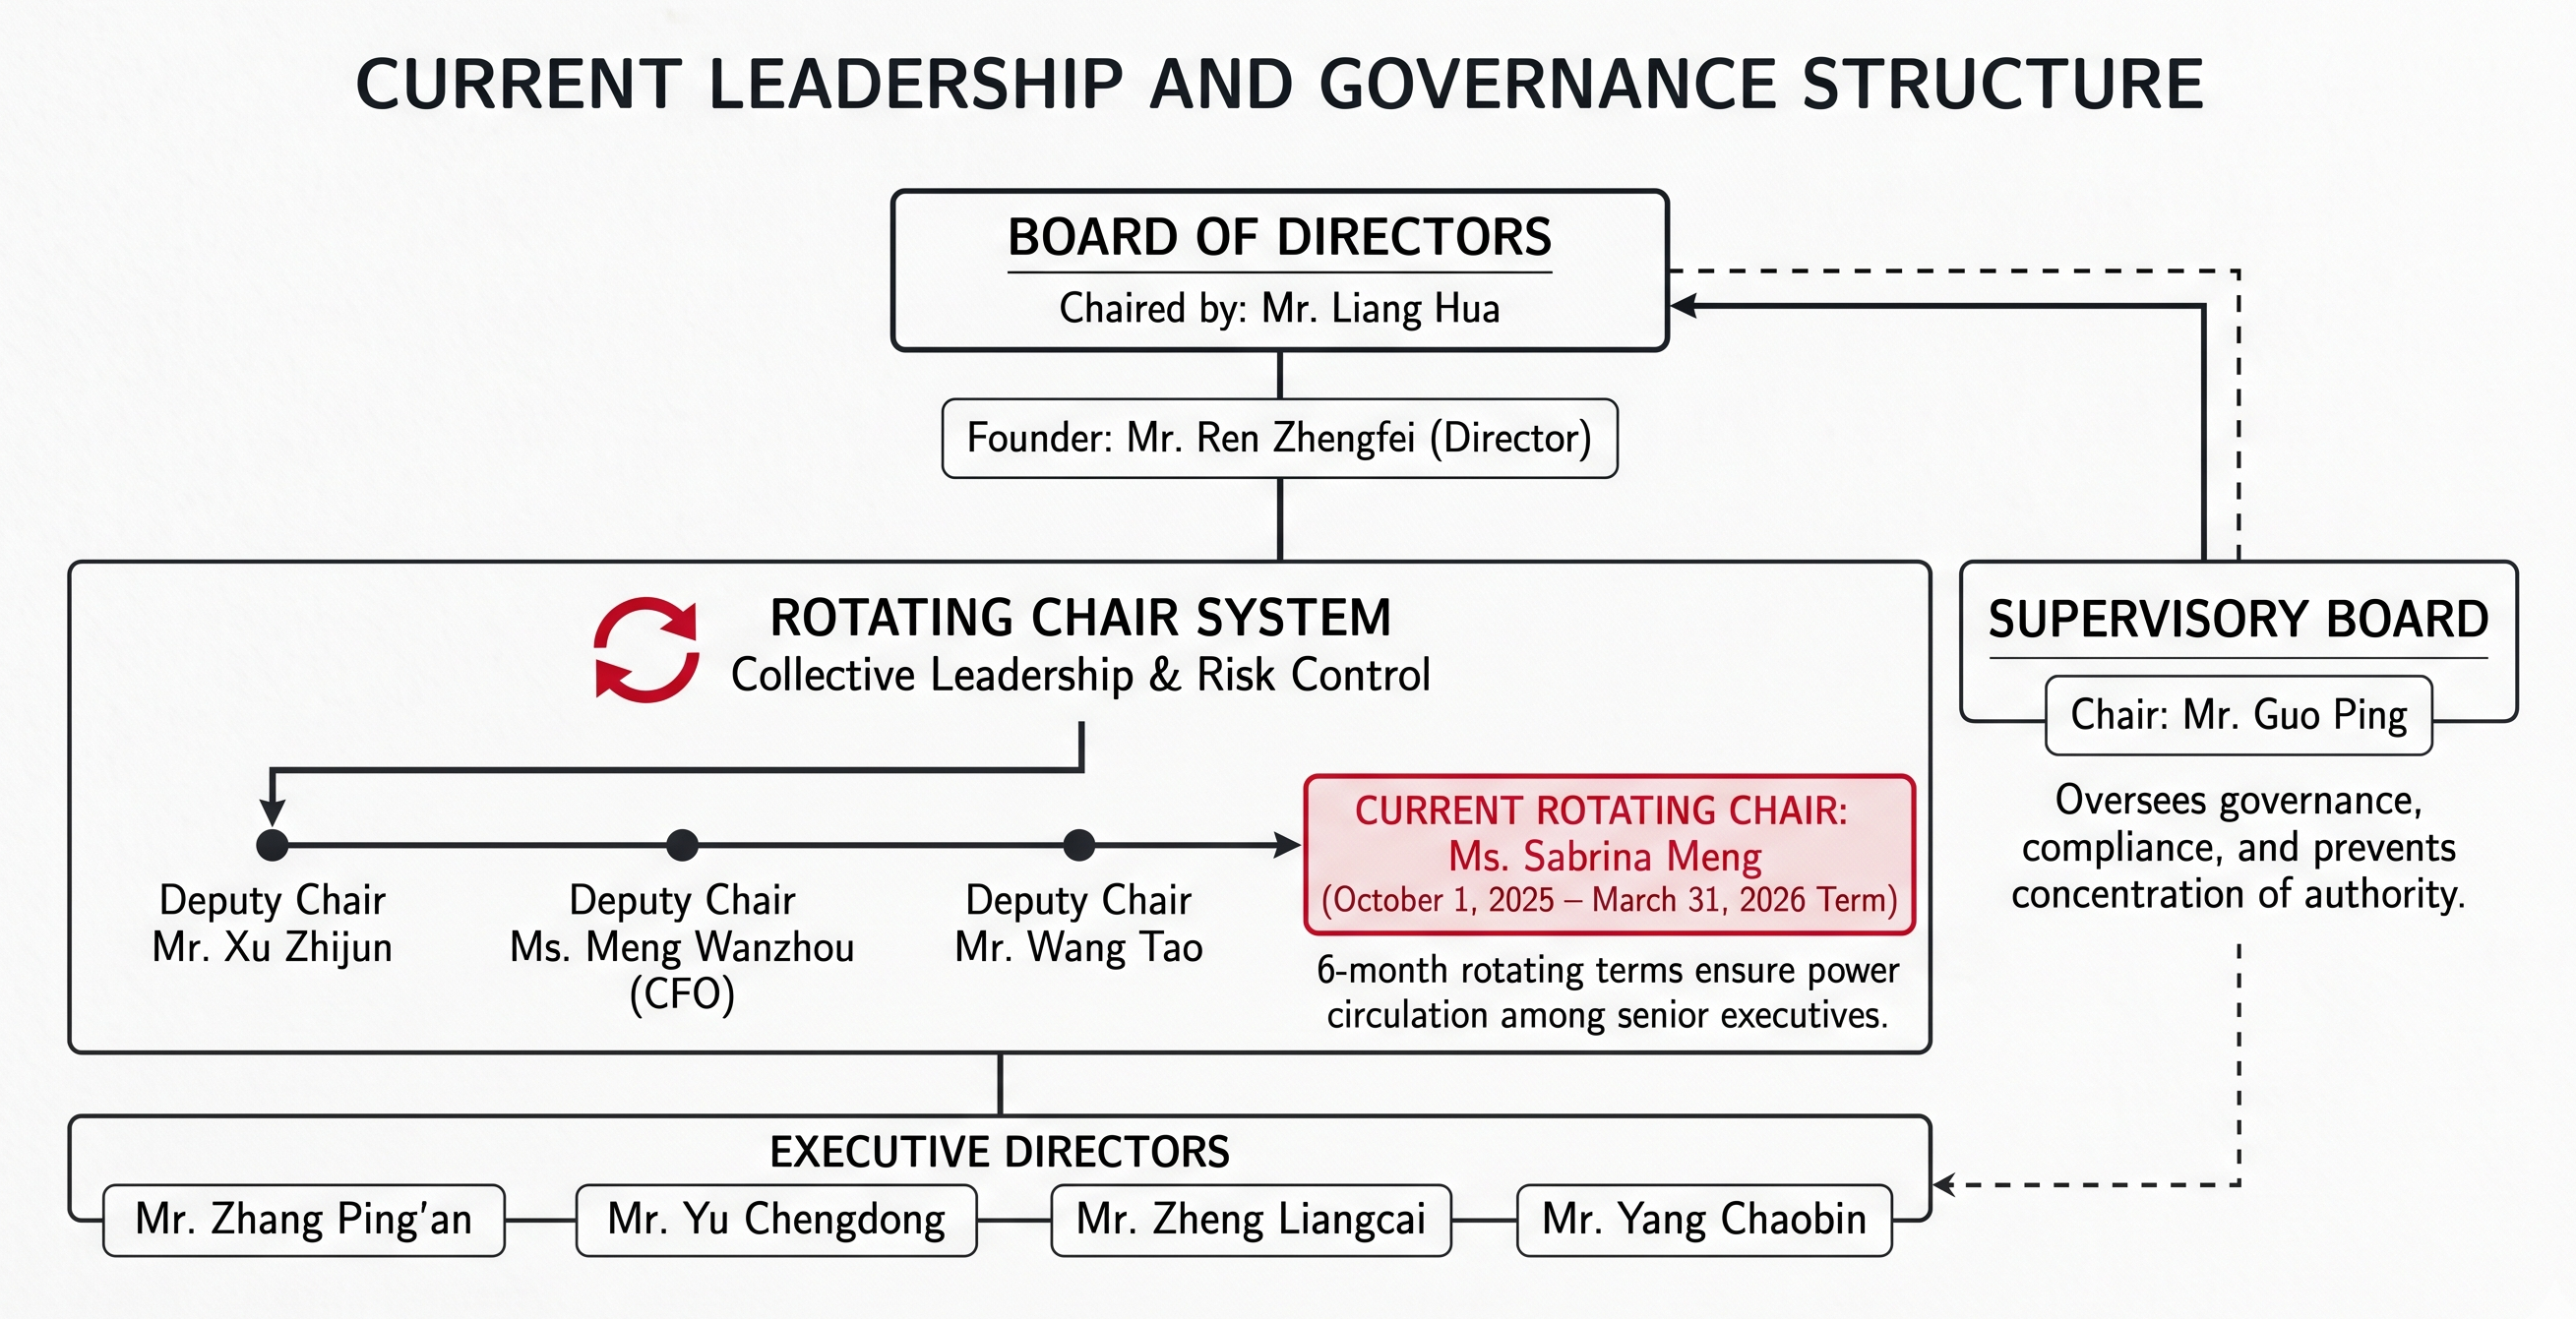
\includegraphics[width=0.8\textwidth]{images/figures/deputy-chairs.png}
    \caption{Rotating Chair System Overview }
    \label{fig:Rotating Chair System Overview }
\end{figure} 


Huawei's operations are organised into four primary Business Groups plus
specialised divisions, as summarised in \tabref{business-groups}.

\begin{table}[htbp]
  \centering
  \caption{Huawei business divisions and key products}
  \label{tab:business-groups}
  \begin{tabularx}{\textwidth}{lX}
    \toprule
    \tableheader{Division & Focus \& Key Products} \\
    \midrule
    Carrier Business Group (\acrshort{cbg})
      & Telecommunications infrastructure: 5G/5G-A base stations, optical
        networks, core networks. Serves 230+ operators worldwide. \\
    \rowcolor{TableRowOdd}
    Enterprise Business Group (\acrshort{ebg})
      & Enterprise \acrshort{ict}: data centres (FusionCube, OceanStor), enterprise
        networking, private 5G, industry cloud solutions. \\
    Consumer Business Group
      & Smart devices: Huawei smartphones (Pura, Mate series), HarmonyOS,
        wearables, tablets. 900M+ HarmonyOS devices (June 2024). \\
    \rowcolor{TableRowOdd}
    Huawei Cloud
      & Public cloud, AI services (Ascend-based instances), industry cloud.
        29 regions globally, 500+ industry scenarios. \\
    AI \& Computing (HiSilicon)
      & Ascend \acrshort{npu}s, Kunpeng processors, MindSpore, \acrshort{cann}.
        Core of Huawei's post-sanctions technological independence strategy. \\
    \rowcolor{TableRowOdd}
    Digital Power
      & Solar inverters, energy storage, EV charging, data centre power systems. \\
    \bottomrule
  \end{tabularx}
\end{table}

% ── 1.3.5 ────────────────────────────────────────────────────
\subsection{Technologies, Products, and Innovation}
\label{subsec:huawei-tech}

Huawei's portfolio spans telecommunications infrastructure, AI computing,
cloud services, consumer devices, and digital power solutions. Key product
families directly relevant to this project are described below.


The Ascend \acrshort{npu} series forms the centrepiece of Huawei's AI computing
strategy. CANN (Compute Architecture for Neural Networks) serves as Huawei's
software abstraction layer analogous to NVIDIA's \acrshort{cuda}, while
MindSpore is an open-source AI training and inference framework supporting
Ascend-native execution. With 4 million developers in the Ascend ecosystem
(2025), Huawei has established a viable alternative to the NVIDIA stack for
Chinese AI infrastructure.

% ── 1.3.6 ────────────────────────────────────────────────────
\subsection{Research \& Development}
\label{subsec:huawei-rd}

Huawei's R\&D commitment is among the most intensive globally. In 2025, the
company invested CNY 192.3 billion (US\$27.5B), representing 21.8\% of annual
revenue — one of the highest R\&D-to-revenue ratios in the global technology
industry. \tabref{rd-investment} summarises recent investment levels.

\begin{table}[htbp]
  \centering
  \caption{Huawei annual R\&D investment (selected years)}
  \label{tab:rd-investment}
  \begin{tabularx}{0.88\textwidth}{lllr}
    \toprule
    \tableheader{Year & R\&D Investment & \% of Revenue & R\&D Employees} \\
    \midrule
    2022 & CNY 161.5B  & 25.1\% & 114,000 \\
    \rowcolor{TableRowOdd}
    2024 & CNY 170.0B  & 21.0\% & 117,150 \\
    2025 & CNY 192.3B  & 21.8\% & 114,000 \\
    \bottomrule
  \end{tabularx}
\end{table}

Huawei has ranked \#1 globally in PCT patent applications for nine consecutive
years (2014–2024), with 165,000+ active granted patents and US\$630 million in
patent licensing revenue in 2024.

% ── 1.3.7 ────────────────────────────────────────────────────
\subsection{Huawei Morocco and Internship Context}
\label{subsec:huawei-morocco}

Huawei has maintained a presence in Morocco since 2007, establishing the
country as the strategic hub for its Northern Africa operations — covering
North, West, and Central Africa. Under the ``In Morocco, For Morocco''
philosophy, Huawei Morocco (Huawei Technologies Morocco S.a.r.l.) serves
as the regional headquarters and actively contributes to Morocco's digital
transformation under the Digital Morocco 2030 programme.


Huawei has partnered with Maroc Telecom, Orange Morocco, and Inwi for 4G/5G
infrastructure deployment — Morocco officially entered the 5G era on
November~7, 2025. The company also supports 54 partner universities through
the Huawei ICT Academy programme, targeting 1,100+ certified students by
2025–2026 across AI, cloud, 5G, and cybersecurity disciplines.

At the 2024 Digital Africa Summit in Marrakech, Huawei committed US\$500M over
five years to expand cloud coverage across Africa, reflecting Morocco's central
role in its continental strategy.

% ============================================================
%  sec-4-technical-context.tex  —  1.4 Technical Context
% ============================================================

\section{Technical Context: AI Infrastructure Evolution}
\label{sec:technical-context}

% ── 1.4.1 ────────────────────────────────────────────────────
\subsection{Introduction to AI Infrastructure}
\label{subsec:ai-infra-intro}

AI infrastructure encompasses the integrated hardware, software, and
system-level components that enable the training, deployment, and operation of
artificial intelligence models at scale. Unlike traditional \acrshort{it}
infrastructure optimised for general-purpose data processing, AI infrastructure
is specifically designed for the massive parallel computational demands of
matrix operations, tensor computations, and neural network workloads.

The infrastructure stack is tightly coupled across four abstraction layers:
hardware, system software, AI frameworks, and orchestration platforms.

AI infrastructure has become a strategic pillar for three interconnected
reasons. First, the AI accelerator market is projected to grow from
\$45B in 2024 to \$500B by 2030 (35\% \acrshort{cagr}), reflecting its
economic significance. Second, NVIDIA's 92\% share of the data centre GPU
market has spurred sovereign AI initiatives in the EU, China, and other regions.
Third, AI computing power has been doubling approximately every 6.8 months —
far exceeding Moore's Law — requiring continuous infrastructure innovation.

% ── 1.4.2 ────────────────────────────────────────────────────
\subsection{Evolution of Computing Architectures}
\label{subsec:arch-evolution}

\subsubsection{CPU Era (1940s–2006)}
\label{subsubsec:cpu-era}

From the 1940s through 2006, \acrfull{cpu}s served as the sole computational
backbone for AI research. While their complex control units excel at
general-purpose branching logic, they face fundamental throughput and bandwidth
limitations for modern parallel AI workloads, as summarised in \tabref{cpu-limits}.

\begin{figure}[H]
    \centering
    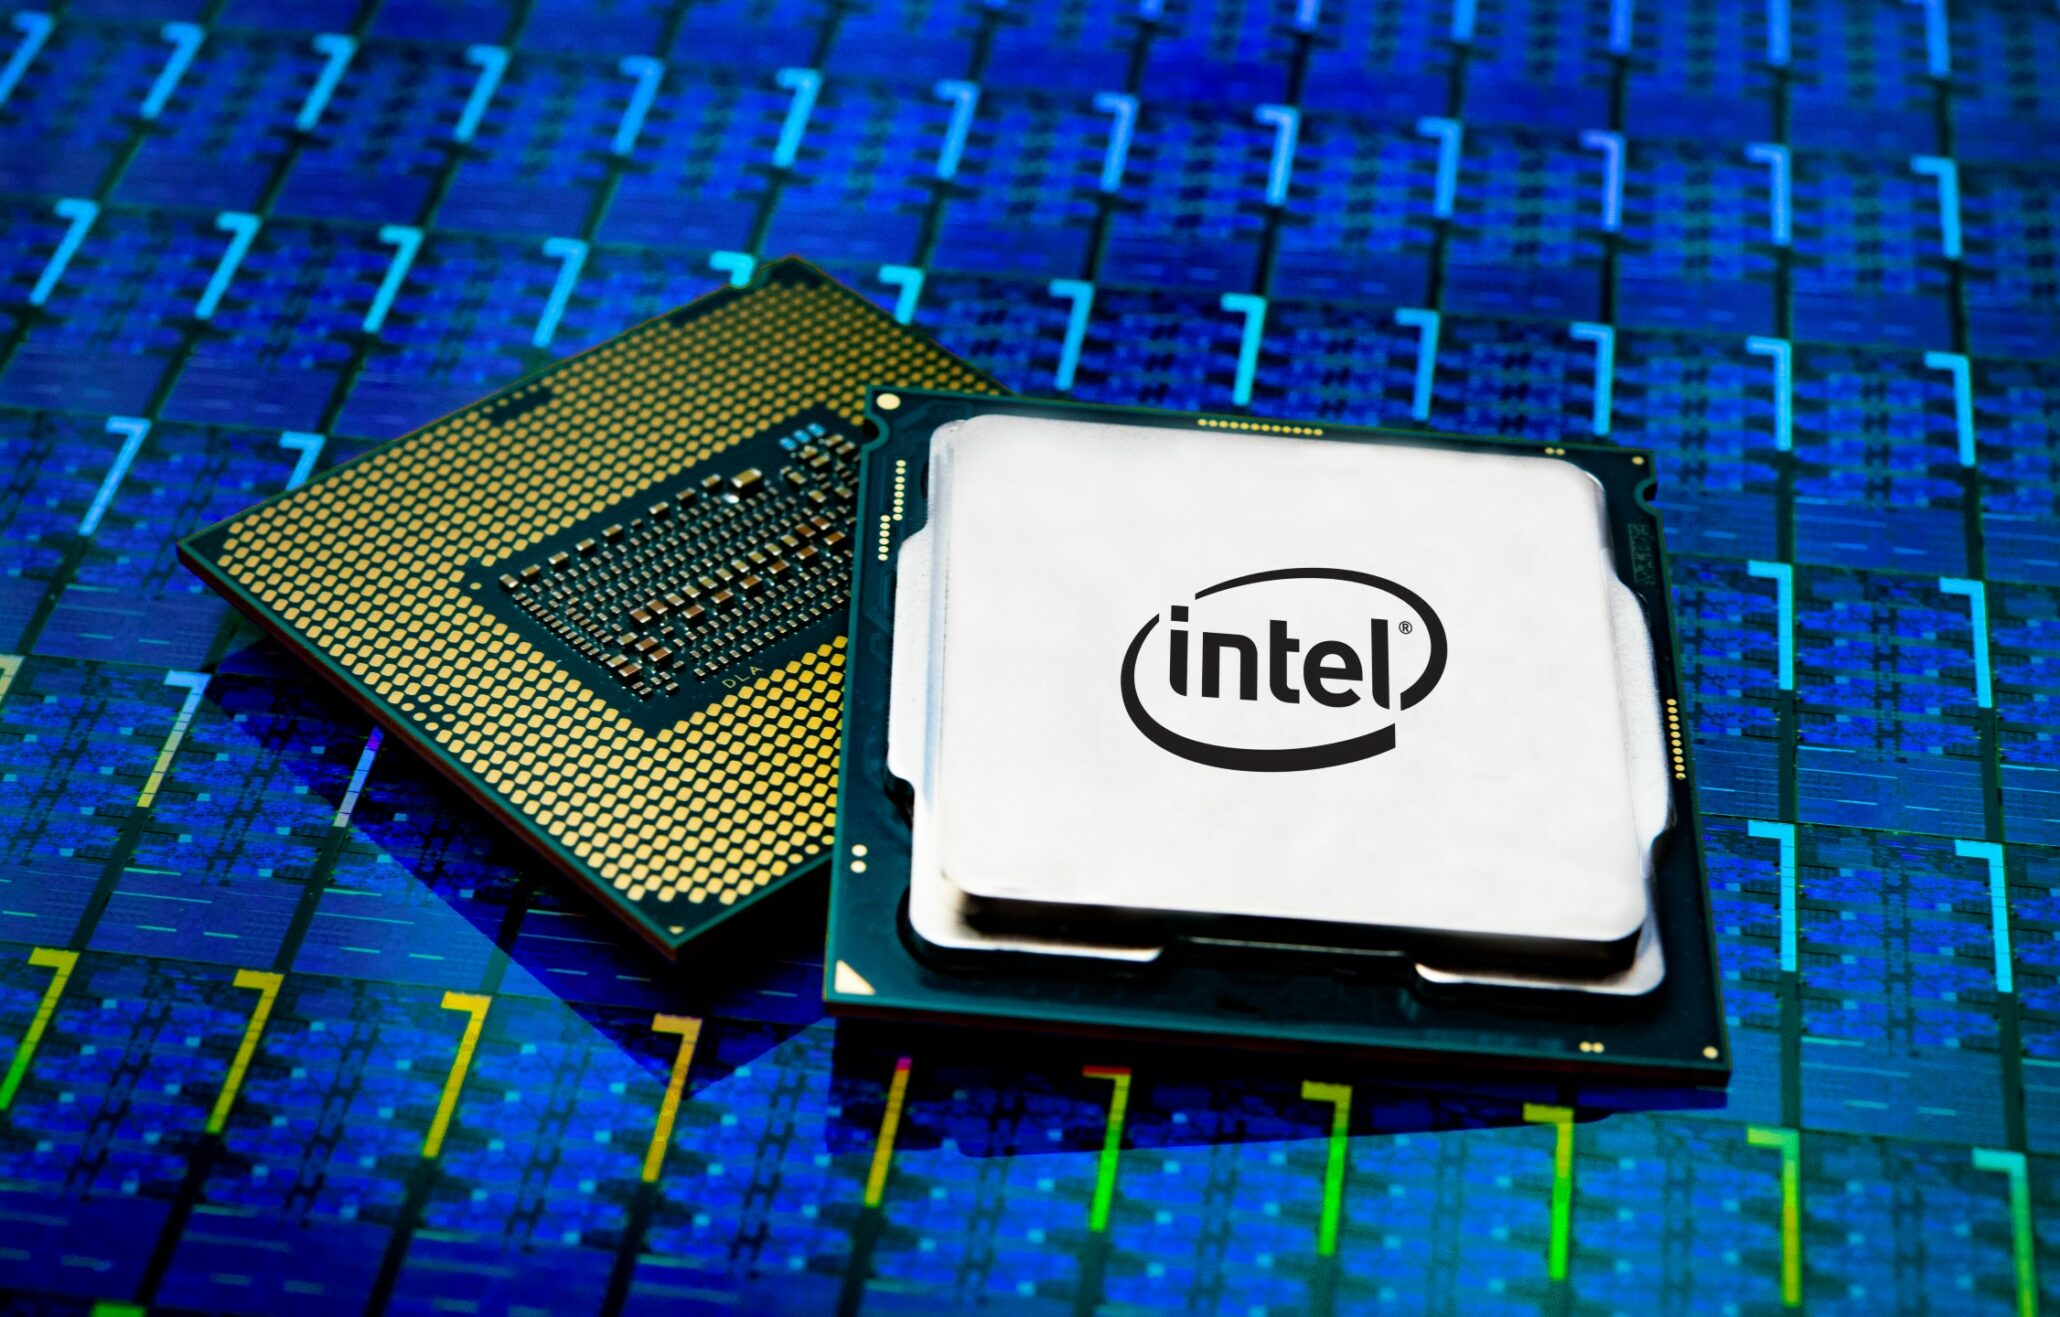
\includegraphics[width=0.5\textwidth]{images/figures/intel-cpu.jpg}
    \caption{Intel CPU Chip}
    \label{fig: Intel CPU Chip}
\end{figure}

\begin{table}[htbp]
  \centering
  \caption{CPU architectural limitations for AI workloads}
  \label{tab:cpu-limits}
  \begin{tabularx}{\textwidth}{lX}
    \toprule
    \tableheader{Limitation & Technical Explanation and AI Impact} \\
    \midrule
    Sequential bottleneck
      & Typical CPUs have 4–96 cores optimised for sequential execution.
        Training ResNet-50 on a CPU takes $\approx$100$\times$ longer than on a GPU. \\
    \rowcolor{TableRowOdd}
    Limited memory bandwidth
      & DDR4/DDR5 bandwidth: 50–200 GB/s — insufficient for large-model
        weight streaming (requires 1–3 TB/s). \\
    Poor FP throughput
      & Single-precision FP32: 0.5–2 TFLOPS; deep learning requires
        tens to hundreds of TFLOPS. \\
    \bottomrule
  \end{tabularx}
\end{table}

\subsubsection{GPU Era (2006–Present)}
\label{subsubsec:gpu-era}

The pivotal transition occurred in 2006 when NVIDIA introduced
\acrfull{cuda}, transforming GPUs from graphics accelerators into
general-purpose parallel processors. The breakthrough moment came in 2012
when AlexNet, trained on GPUs, won ImageNet with 15.3\% top-5 error (vs.\
26.2\% for the best CPU-based approach), demonstrating GPU-accelerated
training 10–100$\times$ faster than CPUs.

Modern data centre GPUs achieve exceptional AI throughput through architectural
features aligned with neural network workloads. The NVIDIA H100, for example,
delivers 989 TFLOPS for FP8 sparse operations with 3,350 GB/s HBM3 memory
bandwidth. The CUDA ecosystem amplified this hardware advantage through a suite
of optimised libraries:

\begin{figure}[H]
    \centering
    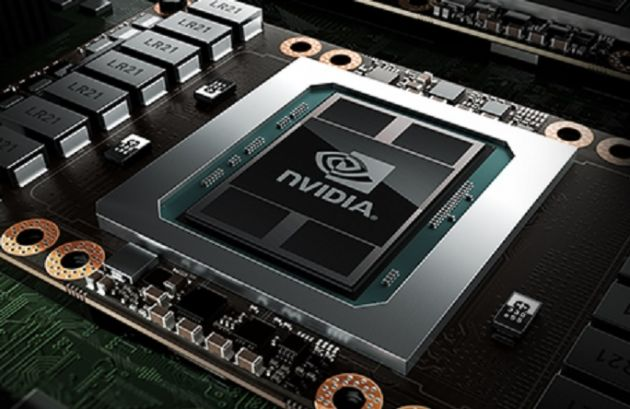
\includegraphics[width=0.5\textwidth]{images/figures/gpu-nvidia.jpg}
    \caption{NVIDIA GPU Chip}
    \label{fig: NVIDIA GPU Chip}
\end{figure}

\begin{table}[htbp]
  \centering
  \caption{Core CUDA ecosystem components and their impact}
  \label{tab:cuda-ecosystem}
  \begin{tabularx}{\textwidth}{llX}
    \toprule
    \tableheader{Component & Function & Performance Impact} \\
    \midrule
    cuDNN     & Deep neural network primitives & 5–10$\times$ speedup for NN operations \\
    \rowcolor{TableRowOdd}
    cuBLAS    & Linear algebra operations       & Foundation for framework optimisations \\
    TensorRT  & Inference optimisation engine   & 3–5$\times$ faster inference \\
    \rowcolor{TableRowOdd}
    NCCL      & Multi-GPU collective communications & Enables distributed training at scale \\
    \bottomrule
  \end{tabularx}
\end{table}

Despite their advantages, GPUs carry inherent limitations: the H100 consumes
700W TDP; training GPT-3 alone required $\approx$1,287 MWh; and a single
DGX H100 system costs \$300,000–\$400,000. Furthermore, approximately 40\%
of GPU transistors are dedicated to graphics features unused in AI workloads.

\subsubsection{Specialised AI Accelerators (NPUs, TPUs, ASICs)}
\label{subsubsec:specialized-accelerators}

Recognising GPU limitations, the industry transitioned toward
Domain-Specific Architectures (\acrshort{dsa}s). Google accelerated this
shift with its Tensor Processing Unit (\acrshort{tpu}) in 2015 — an ASIC
designed exclusively for tensor computations. \tabref{accelerator-comparison}
compares key accelerator specifications.

\begin{figure}[H]
    \centering
    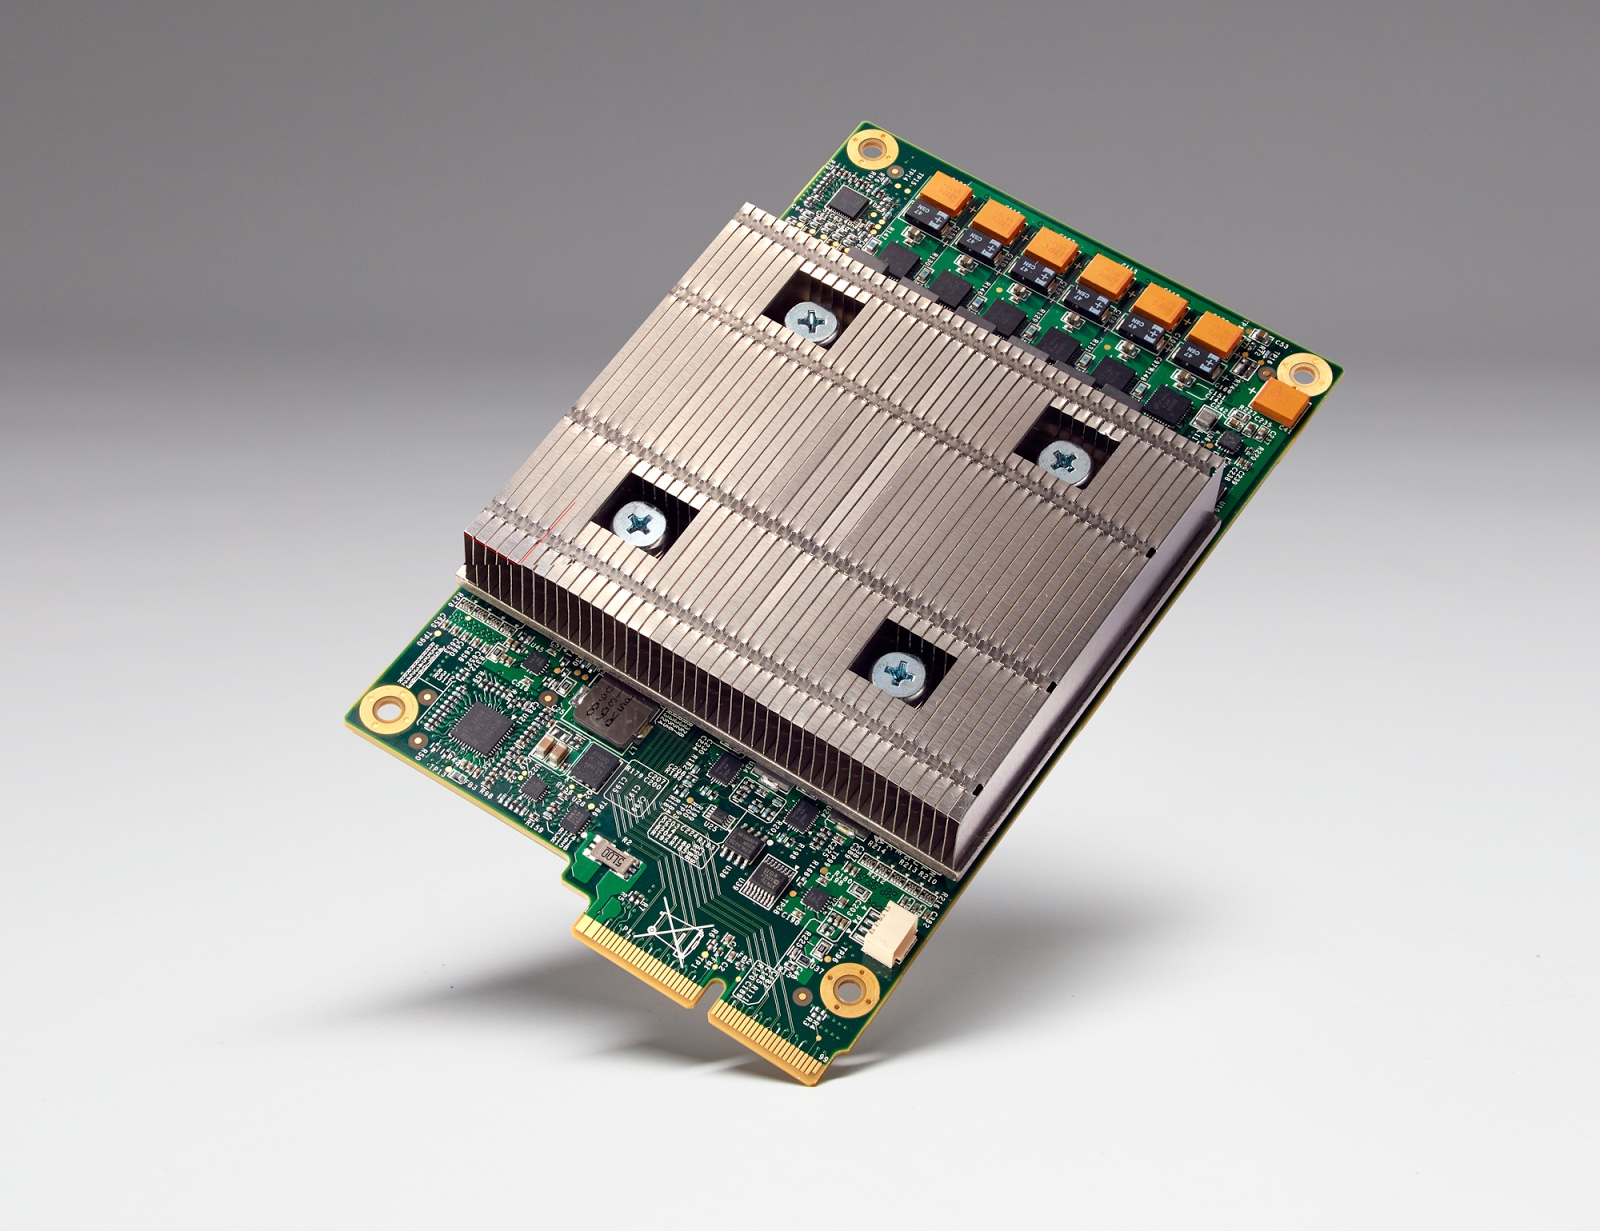
\includegraphics[width=0.5\textwidth]{images/figures/tpu.jpg}
    \caption{Google TPU Chip}
    \label{fig: Google TPU Chip}
\end{figure}

\begin{table}[htbp]
  \centering
  \caption{Comparative specifications: GPU vs. NPU vs. ASIC}
  \label{tab:accelerator-comparison}
  \begin{tabularx}{\textwidth}{lXXX}
    \toprule
    \tableheader{Attribute & GPU (H100) & NPU (Ascend 910B) & ASIC (TPU v4)} \\
    \midrule
    Architecture   & General parallel + graphics & Pure tensor accelerator & Fixed-function \\
    \rowcolor{TableRowOdd}
    Peak FP16      & 989 TFLOPS                 & 256 TFLOPS             & 275 TFLOPS \\
    Memory / BW    & 80 GB HBM3, 3,350 GB/s    & 64 GB HBM2, 1,200 GB/s & 32 GB HBM2 \\
    \rowcolor{TableRowOdd}
    TDP            & 700 W                      & 310 W                  & 170 W \\
    Efficiency     & $\approx$1.5 TOPS/W        & $\approx$3–4 TOPS/W    & $\approx$5 TOPS/W \\
    \rowcolor{TableRowOdd}
    Ecosystem      & CUDA (mature, proprietary) & CANN (Huawei)          & XLA/JAX (Google) \\
    \bottomrule
  \end{tabularx}
\end{table}

% ── 1.4.3 ────────────────────────────────────────────────────
\subsection{Increasing AI Computational Demands}
\label{subsec:compute-demands}

The exponential growth in AI compute demands has been the primary driver
behind the hardware evolution described above. From AlexNet (2012) to GPT-4
(2023), parameter counts increased from 60 million to an estimated 1.7
trillion — a 28,000$\times$ increase. Training compute grew even more
dramatically, from approximately $10^{16}$ FLOPs to beyond $10^{25}$ FLOPs —
a billion-fold increase in just eleven years.

This multiplicative structure means that both model size and data scale
jointly drive training cost. \tabref{model-compute} illustrates the growth trajectory.

\begin{table}[htbp]
  \centering
  \caption{Growth in training compute for landmark models}
  \label{tab:model-compute}
  \begin{tabularx}{\textwidth}{lllll}
    \toprule
    \tableheader{Model & Year & Parameters & Training FLOPs & Dataset} \\
    \midrule
    AlexNet & 2012 & 60M    & $\sim$$10^{16}$ & 1.2M images \\
    \rowcolor{TableRowOdd}
    GPT-2   & 2019 & 1.5B   & $\sim$$10^{21}$ & 40 GB text \\
    GPT-3   & 2020 & 175B   & $3.1 \times 10^{23}$ & 300B tokens \\
    \rowcolor{TableRowOdd}
    PaLM    & 2022 & 540B   & $6.5 \times 10^{24}$ & 780B tokens \\
    GPT-4   & 2023 & $\sim$1.7T & $>$$10^{25}$ & $\sim$13T tokens \\
    \bottomrule
  \end{tabularx}
\end{table}

This growth rate — doubling roughly every 6.8 months — far exceeds historical
Moore's Law (18–24 months per doubling) and creates an energy and cost crisis.
Training GPT-3 consumed $\approx$1,287 MWh and cost $\approx$\$4.6M in cloud
compute; GPT-4 is estimated at \$63–78M. Data centre AI power demand is
projected to more than double by 2030, potentially reaching 94.5 GW globally.

% ── 1.4.4 ────────────────────────────────────────────────────
\subsection{GPU Ecosystem Dominance}
\label{subsec:gpu-dominance}

NVIDIA commands approximately 92\% of the data centre GPU market as of 2024,
a position built on three interlocking advantages: (1) the CUDA software stack
with 4+ million developers and a decade-and-a-half head start; (2) continuous
architectural innovation (Volta $\to$ Turing $\to$ Ampere $\to$ Hopper $\to$
Blackwell); and (3) a mature developer ecosystem where over 95\% of papers at
top AI conferences use NVIDIA hardware, creating reproducibility norms that
reinforce adoption.

\begin{figure}[H]
    \centering
    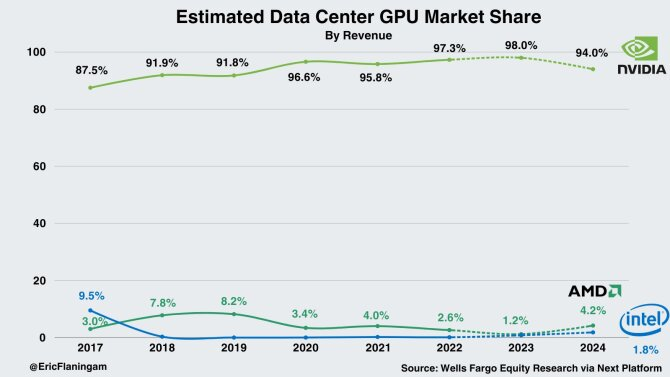
\includegraphics[width=0.7\textwidth]{images/figures/GPU-market-share.jpg}
    \caption{GPU Market Share 2024}
    \label{fig: GPU Market Share 2024}
\end{figure}

This dominance, however, carries systemic risks. CUDA is proprietary and
NVIDIA-exclusive, creating prohibitive migration costs for organisations with
large CUDA codebases. H100 GPUs sell at \$25,000–\$40,000 per unit and carry
36–52 week delivery lead times. Training large models requires
multi-node clusters drawing hundreds of megawatts. Communication overhead can
consume 30–50\% of training time in large clusters without specialised
interconnects. US export restrictions on advanced AI chips to China (2022–2023)
further exposed the fragility of a single-vendor, single-geography ecosystem.

% ── 1.4.5 ────────────────────────────────────────────────────
\subsection{Hardware Specialisation Trends}
\label{subsec:hw-specialisation}

The semiconductor industry is undergoing a fundamental shift from
general-purpose to domain-specific architectures, driven by the convergence
of three constraints: the end of Moore's Law scaling, energy efficiency
boundaries, and the specialised computational patterns of AI workloads.

At process nodes below 5nm, quantum tunnelling effects and manufacturing
complexity make further density increases prohibitively expensive. Meanwhile,
AI workloads exhibit highly regular computational patterns — over 90\%
matrix multiplications and convolutions — that general-purpose processors
cannot exploit efficiently.

\begin{table}[htbp]
  \centering
  \caption{Architectural comparison across computing paradigms}
  \label{tab:arch-comparison}
  \begin{tabularx}{\textwidth}{lXXX}
    \toprule
    \tableheader{Criterion & CPU & GPU & NPU/ASIC} \\
    \midrule
    Parallelism   & Sequential + limited parallel & Thousands of cores  & Systolic arrays, MAC units \\
    \rowcolor{TableRowOdd}
    Precision     & FP32/FP64                    & FP16/FP32           & INT8/FP16 optimised \\
    Power (data centre) & 65–350W               & 300–700W            & 10–310W \\
    \rowcolor{TableRowOdd}
    Efficiency    & $\approx$0.1 TOPS/W          & $\approx$2 TOPS/W   & 5–50+ TOPS/W \\
    Best use case & Control logic, preprocessing & Training, batch inf. & Inference, edge AI \\
    \bottomrule
  \end{tabularx}
\end{table}

The AI computing landscape is bifurcating into cloud (training and large-scale
batch inference) and edge (real-time, low-latency inference) domains, each with
distinct hardware requirements.

% ── 1.4.6 ────────────────────────────────────────────────────
\subsection{Rise of Neural Processing Units}
\label{subsec:npu-rise}

A Neural Processing Unit is a specialised microprocessor explicitly designed
to accelerate AI and machine learning workloads by implementing the
mathematical structure of neural networks directly in silicon. NPUs incorporate
thousands of multiply-accumulate (\acrshort{mac}) units arranged in systolic
array patterns, enabling massive parallel matrix multiplication — the
fundamental operation in deep learning.



% ============================================================
%  sec-5-project-motivation.tex  —  1.5 Project Motivation
% ============================================================

\section{Project Motivation}
\label{sec:project-motivation}

The proliferation of generative AI and large-scale machine learning workloads
has fundamentally transformed modern computing infrastructure. Organisations
worldwide are investing heavily in AI-capable data centres, yet the prevailing
reliance on \acrshort{gpu}-dominated infrastructures has revealed critical
limitations in cost, energy efficiency, supply chain resilience, and strategic
autonomy. This project addresses the urgent industrial need for structured
methodologies to evaluate, guide, and optimise the migration from GPU-centric
architectures toward \acrshort{npu}-based alternatives.

% ── 1.5.1 ────────────────────────────────────────────────────
\subsection{Need for GPU\texorpdfstring{$\,\to\,$}{-to-}NPU Migration Guidance}
\label{subsec:migration-need}

Since the advent of deep learning, \acrfull{gpu}s have established themselves
as the de facto hardware foundation for AI workloads, with the market projected
to reach USD 228.04B by 2030.

\subsubsection{Structural Limitations Driving Migration}

Despite this dominance, the GPU-centric paradigm is increasingly
unsustainable. \tabref{gpu-limitations} summarises the five structural
limitations that motivate the exploration of NPU-based alternatives.

\begin{table}[htbp]
  \centering
  \caption{Structural limitations of GPU-centric AI infrastructure}
  \label{tab:gpu-limitations}
  \begin{tabularx}{\textwidth}{lX}
    \toprule
    \tableheader{Limitation & Key Evidence} \\
    \midrule
    Energy consumption
      & A single GB200 NVL72 rack draws 120–132 kW vs.\ 10–15 kW for a typical
        enterprise rack; AI's energy needs projected at 21\% of global
        electricity by 2030. \\
    \rowcolor{TableRowOdd}
    Infrastructure cost
      & Data centre construction costs rose from \$7.7M to \$10.7M per MW
        between 2020 and 2025 (7\% CAGR). \\
    Vendor lock-in
      & CUDA's dominance creates prohibitive migration barriers; multi-year supply
        agreements between NVIDIA and hyperscalers crowd out enterprise buyers. \\
    \rowcolor{TableRowOdd}
    Scalability for mid-size enterprises
      & Four GB200 racks require $\approx$0.5 MW of dedicated power plus
        liquid cooling infrastructure unavailable in most enterprise data centres. \\
    Supply chain constraints
      & GPU delivery windows stretch 36–52 weeks; Blackwell-class hardware
        delayed to Q1 2027; NVIDIA consumes $\approx$60\% of CoWoS packaging
        capacity. \\
    \bottomrule
  \end{tabularx}
\end{table}

NPUs address these limitations through domain-specific architectures.
Recent benchmarks show NPUs delivering 30–63\% higher energy efficiency than
NVIDIA GPUs in quantised \acrshort{llm} inference, while operating at
10–30W per chip compared to 300–700W for data centre GPUs.

\subsubsection{Enterprise Migration Challenges}

Despite the promise of NPUs, enterprises face significant migration barriers:
GPU-oriented ecosystems, unclear migration paths, limited NPU expertise, and
workload heterogeneity (training vs.\ inference, latency vs.\ throughput, cloud
vs.\ edge). The absence of structured guidance creates a systematic gap between
the theoretical advantages of NPU adoption and practical deployment capability.
This project directly addresses this gap.

% ── 1.5.2 ────────────────────────────────────────────────────
\subsection{Need for Compatibility Analysis}
\label{subsec:compatibility-need}

Compatibility analysis is a critical technical prerequisite during AI hardware
transitions. The shift from GPU to NPU is not merely a hardware substitution
but a fundamental reconfiguration of the entire software-hardware stack. A 2025
industry analysis found that 68\% of production AI workloads contain at least
one CUDA-dependent component requiring manual reimplementation for NPU
deployment, rising to 85\% for workloads using custom architectures.

\subsubsection{Software Compatibility Dimensions}

\begin{table}[htbp]
  \centering
  \caption{AI framework compatibility status across hardware backends}
  \label{tab:framework-compat}
  \begin{tabularx}{\textwidth}{llXl}
    \toprule
    \tableheader{Framework & Primary Backend & NPU Support Status & Migration Complexity} \\
    \midrule
    PyTorch      & CUDA (NVIDIA)    & Limited (requires CANN/MindSpore adaptation) & High \\
    \rowcolor{TableRowOdd}
    TensorFlow   & CUDA (NVIDIA)    & Partial (via Ascend TF plugin)               & Medium-High \\
    MindSpore    & Ascend NPU       & Native                                       & Low \\
    \rowcolor{TableRowOdd}
    ONNX Runtime & Multi-arch       & Moderate (provider-dependent)                & Medium \\
    \bottomrule
  \end{tabularx}
\end{table}

CUDA creates dependency at multiple abstraction levels simultaneously:
custom CUDA kernels, cuDNN/cuBLAS libraries, profiling tools (Nsight), and
model checkpoint formats with CUDA-specific metadata. Each layer must be
validated independently during migration.

\subsubsection{Impact of Compatibility Problems}

Compatibility failures affect four dimensions of deployment success.
\textbf{Feasibility}: severe incompatibilities can render deployment impossible
without prohibitive re-engineering — cases include models with proprietary
CUDA kernels and framework versions incompatible with NPU drivers.
\textbf{Performance}: suboptimal operator implementations may reduce throughput
by 30–50\% and increase latency through memory layout mismatches.
\textbf{Maintenance complexity}: organisations maintaining both GPU and NPU
infrastructure must support two complete, evolving software stacks.
\textbf{Cost}: industry estimates suggest 40–60\% of total migration cost
arises from software compatibility resolution, not hardware procurement.

Such migrations require not only code changes but framework-level retraining,
model checkpoint conversion, and accuracy validation — illustrating the need
for systematic compatibility analysis methodologies.

% ── 1.5.3 ────────────────────────────────────────────────────
\subsection{Need for Hardware Transition Evaluation}
\label{subsec:evaluation-need}

Hardware transition decisions represent multi-year infrastructure commitments
that shape organisational AI capabilities. Systematic evaluation must span
five complementary dimensions.

\subsubsection{Performance Benchmarking}

GPU and NPU performance profiles differ fundamentally across workload types.
For inference at batch size 1, NPUs can achieve 3–10$\times$ lower latency
than GPUs. For large-scale training, GPUs remain significantly superior.
Benchmarks must be conducted under realistic production conditions — including
data pipeline overhead, network latency, and memory contention — not idealised
laboratory settings.

This project addresses the need for systematic methodologies, enabling
organisations to make data-driven infrastructure decisions based on
comprehensive technical and economic assessment rather than incomplete
information or vendor marketing claims.



\blankpage
% ============================================================
%  chapters/02-technological-background/chapter.tex
%  Chapter 2 — Technological Background
% ============================================================

\chapter{Technological Background}
\label{chap:tech-background}

% ============================================================
%  sec-1-gpu-foundations.tex  —  2.1 GPU Computing Foundations
% ============================================================

\section{GPU Computing Foundations}
\label{sec:gpu-foundations}

Graphics Processing Units have evolved from specialised graphics accelerators
into the dominant computational paradigm for modern AI, enabling the training
of deep neural networks at scales that would be infeasible on traditional
\acrshort{cpu} architectures. The transition began with NVIDIA's 2006
introduction of \acrshort{cuda}, which decoupled GPU computing from graphics
\acrshort{api}s and enabled direct programmability for scientific and AI
workloads. Since then, frameworks such as PyTorch and TensorFlow achieve their
GPU performance through \acrshort{cuda}-accelerated libraries — cuBLAS, cuDNN
— making GPU computing not merely advantageous but essential for contemporary
AI systems.

The fundamental architectural distinction between CPUs and GPUs reflects
different design philosophies: CPUs are latency-oriented, optimised for
completing individual tasks quickly through complex control logic; GPUs are
throughput-oriented, designed to process large data volumes in parallel by
sacrificing single-thread performance for aggregate concurrency. This
distinction is quantified in \tabref{cpu-vs-gpu}.

\begin{table}[htbp]
  \centering
  \caption{CPU vs. GPU architectural characteristics}
  \label{tab:cpu-vs-gpu}
  \begin{tabularx}{\textwidth}{lXX}
    \toprule
    \tableheader{Feature & CPU & GPU} \\
    \midrule
    Design philosophy  & Latency-oriented      & Throughput-oriented \\
    \rowcolor{TableRowOdd}
    Core count         & 4–96 cores            & Hundreds to thousands of cores \\
    Control logic      & Complex (branch pred., out-of-order) & Simplified (repetitive parallel ops) \\
    \rowcolor{TableRowOdd}
    Memory bandwidth   & 50–100 GB/s           & 200–3,350 GB/s \\
    Thread parallelism & Dozens of threads     & 10,000+ concurrent threads \\
    \rowcolor{TableRowOdd}
    Cache hierarchy    & Large L1/L2/L3        & Smaller caches; compensated by bandwidth \\
    \bottomrule
  \end{tabularx}
\end{table}

% ── 2.1.1 ────────────────────────────────────────────────────
\subsection{CUDA Architecture Overview}
\label{subsec:cuda-arch}

\acrfull{cuda} is NVIDIA's parallel computing platform and programming model,
introduced in 2006 alongside the GeForce 8-series. Before CUDA, exploiting
GPU compute required embedding algorithms inside graphics shader code — a
severely limiting constraint. CUDA unified the shader architecture into
programmable ``CUDA cores'' and exposed GPU parallelism through a C-like
programming interface, establishing it as the \textit{de facto} standard for
\acrshort{gpu} computing.

\begin{figure}[H]
    \centering
    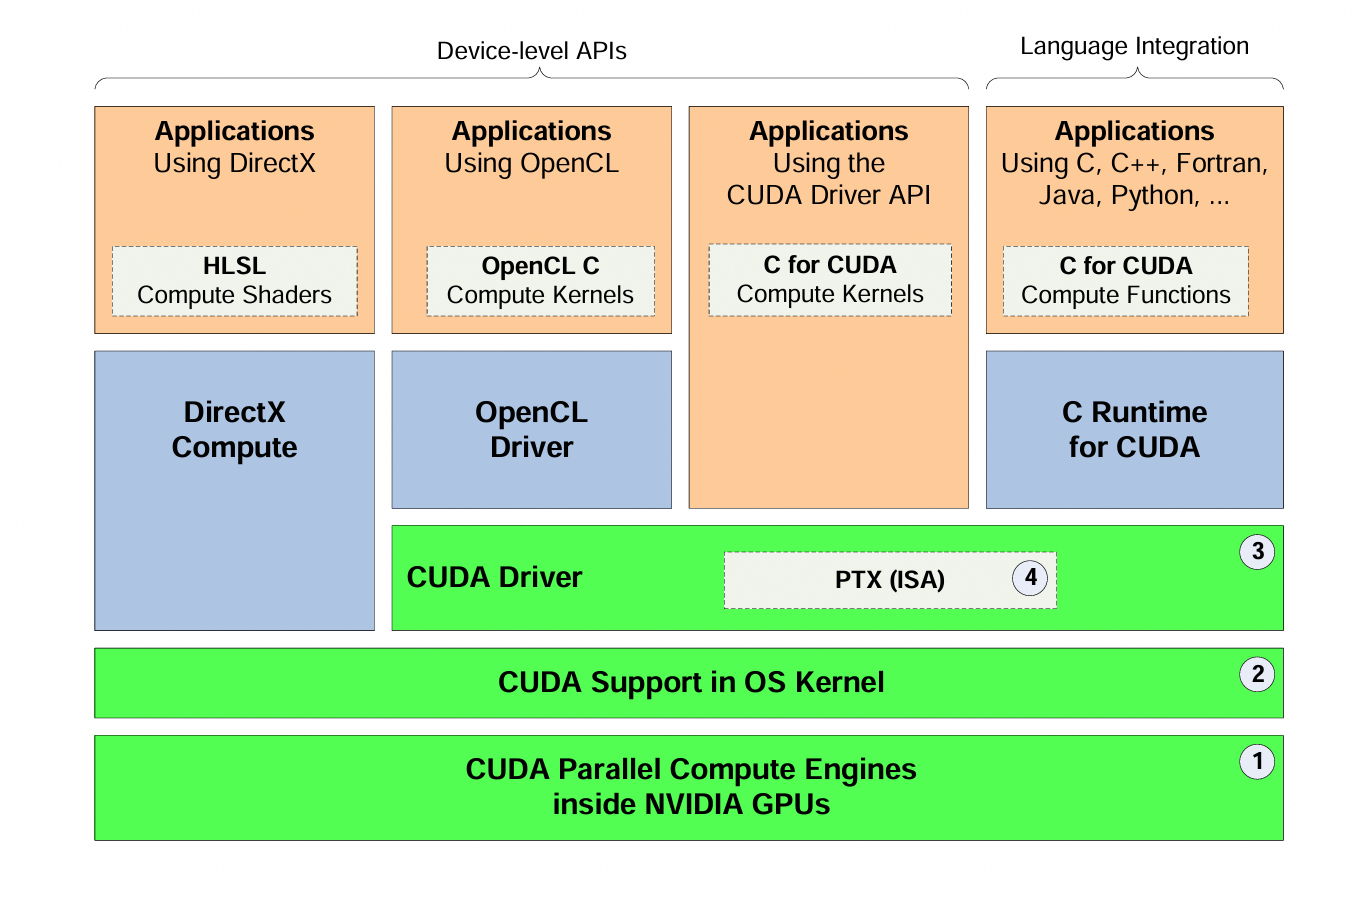
\includegraphics[width=0.85\textwidth]{images/figures/cuda-architecture.png}
    \caption{CUDA Architecture Overview}
    \label{fig: CUDA Architecture Overview}
\end{figure}

\subsubsection{Streaming Multiprocessors}
\label{subsubsec:sms}

The \acrfull{sm} is the fundamental autonomous execution unit of any NVIDIA
GPU. Each SM contains: CUDA cores (FP32/INT32 execution); Tensor Cores
(matrix multiply-accumulate, introduced in Volta 2017); warp schedulers
(typically 4 per SM); a large register file (32K–64K registers per SM
enabling zero-overhead context switching); configurable shared memory /
L1 cache (48–96 KB per SM); and special function units (SFUs) for
transcendental operations.

For reference, the NVIDIA A100 contains 108 SMs with 64 CUDA cores each
— totalling 6,912 cores — and can manage up to 2,048 threads per SM
simultaneously, grouped into 64 warps of 32 threads.

\subsubsection{SIMT Execution and Warp Model}
\label{subsubsec:simt}

CUDA implements the \acrfull{simt} model: groups of 32 consecutive threads
called \textit{warps} execute the same instruction in lock-step, each
operating on different data. Key properties of warp execution are:

\begin{itemize}
  \item All 32 threads in a warp execute the same instruction simultaneously.
  \item The warp scheduler switches between warps with zero overhead when
        one warp awaits memory — this is the primary latency-hiding mechanism.
  \item \textbf{Branch divergence}: when threads within a warp follow different
        execution paths, the warp serialises each path, potentially reducing
        throughput by up to 50\%.
  \item Each SM can manage 64 warps (2,048 threads) but dispatches typically
        4 warps per cycle through its warp schedulers.
\end{itemize}

% ── 2.1.2 ────────────────────────────────────────────────────
\subsection{CUDA Execution Model}
\label{subsec:cuda-execution}

\subsubsection{Thread Hierarchy}

CUDA organises threads into a two-level hierarchy. \textbf{Thread blocks}
are groups of threads that share data through shared memory and can
synchronise via barriers (\texttt{\_\_syncthreads()}). Block sizes are
multiples of 32 for warp alignment — typically 128, 256, or 512. A
\textbf{grid} is the collection of all thread blocks executing a kernel.
Each thread computes its unique global identifier as:
\begin{equation}
  i = \texttt{blockIdx.x} \times \texttt{blockDim.x} + \texttt{threadIdx.x}
  \label{eq:thread-id}
\end{equation}

\begin{figure}[H]
    \centering
    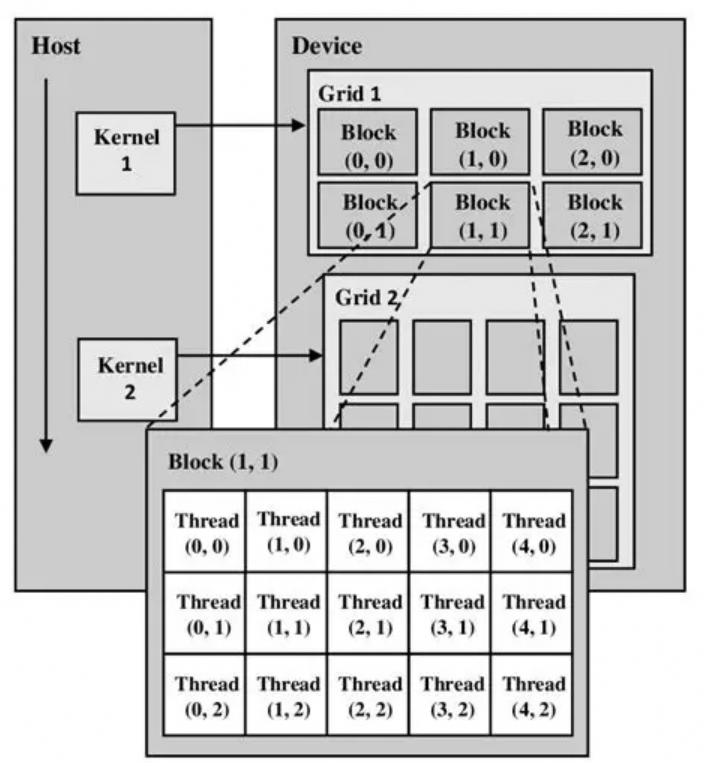
\includegraphics[width=0.85\textwidth]{images/figures/kernel-execution.png}
    \caption{Kernel Execution Flow}
    \label{fig:cuda-kernel-flow}
\end{figure}


% ── 2.1.3 ────────────────────────────────────────────────────
\subsection{CUDA Memory Hierarchy}
\label{subsec:cuda-memory}

CUDA exposes a multi-level memory hierarchy whose performance implications
are central to kernel optimisation. \tabref{cuda-memory} summarises the
key characteristics of each level.

\begin{table}[htbp]
  \centering
  \caption{CUDA memory hierarchy: latency, bandwidth, and scope}
  \label{tab:cuda-memory}
  \begin{tabularx}{\textwidth}{llllX}
    \toprule
    \tableheader{Memory Type & Scope & Capacity & Latency & Bandwidth} \\
    \midrule
    Registers      & Per-thread & $\sim$255 regs & $\sim$1 cycle  & $\sim$8 TB/s \\
    \rowcolor{TableRowOdd}
    Shared Memory  & Per-block  & 48–96 KB/SM  & 20–30 cycles & $>$1 TB/s \\
    L1 Cache       & Per-SM     & 16–48 KB/SM  & 20–30 cycles & $\sim$1 TB/s \\
    \rowcolor{TableRowOdd}
    L2 Cache       & Per-GPU    & 4–6 MB       & Tens of cycles & Moderate \\
    Global Memory  & Per-GPU    & 8–80 GB      & 400–800 cycles & 200–3,350 GB/s \\
    \rowcolor{TableRowOdd}
    Constant Mem.  & Per-GPU    & 64 KB        & $\sim$1 cycle (cached) & $\sim$800 GB/s \\
    \bottomrule
  \end{tabularx}
\end{table}

Three optimisation principles govern GPU memory performance. First,
\textbf{memory coalescing}: consecutive threads should access consecutive
addresses so the hardware merges accesses into fewer transactions —
strided access patterns can reduce effective throughput by 10–50$\times$.
Second, \textbf{shared memory tiling}: caching frequently reused data in
shared memory (20–30 cycle latency) avoids repeated 400–800 cycle global
memory round-trips, which is critical for tiled matrix multiplication and
convolution. Third, \textbf{register pressure}: excessive register usage
reduces occupancy (active warps per SM), limiting the scheduler's ability
to hide global memory latency — maintaining above 50\% occupancy is
typically the target.

% ── 2.1.4 ────────────────────────────────────────────────────
\subsection{CUDA Ecosystem and Software Stack}
\label{subsec:cuda-ecosystem}

CUDA's dominance in AI infrastructure is as much a software phenomenon as
a hardware one. The CUDA Toolkit provides a complete development
environment: the \texttt{nvcc} compiler, profiling tools (Nsight Systems,
Nsight Compute), and a suite of hand-tuned libraries summarised in
\tabref{cuda-libs}.

\begin{figure}[H]
    \centering
    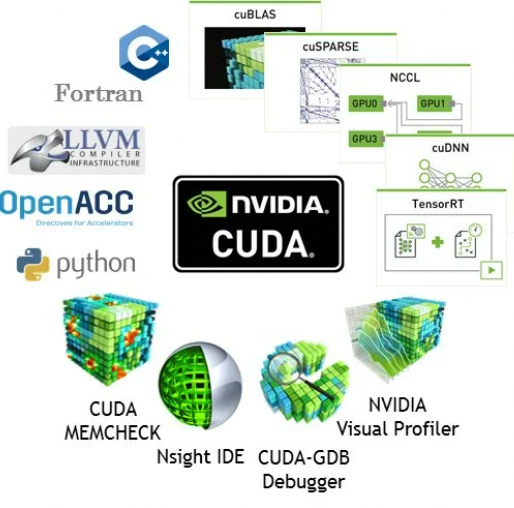
\includegraphics[width=0.85\textwidth]{images/figures/cuda-ecosystem.png}
    \caption{CUDA Ecosystem Overview}
    \label{fig:cuda-ecosystem}
\end{figure}

\begin{table}[htbp]
  \centering
  \caption{Core CUDA libraries and their relevance to AI workloads}
  \label{tab:cuda-libs}
  \begin{tabularx}{\textwidth}{llX}
    \toprule
    \tableheader{Library & Function & AI Relevance} \\
    \midrule
    cuDNN    & Deep neural network primitives & Conv, pooling, normalisation, RNN; 5–10$\times$ speedup \\
    \rowcolor{TableRowOdd}
    cuBLAS   & Basic linear algebra           & Matrix multiplication for all linear layers \\
    NCCL     & Collective communications       & Multi-GPU gradient synchronisation \\
    \rowcolor{TableRowOdd}
    TensorRT & Inference optimisation          & Layer fusion, quantisation; 3–5$\times$ faster inference \\
    CUTLASS  & Templated GEMM kernels          & Custom matrix operations for novel architectures \\
    \bottomrule
  \end{tabularx}
\end{table}

PyTorch and TensorFlow achieve GPU acceleration by dispatching operations to
these libraries rather than implementing custom kernels. Over 95\% of papers
at top AI venues (NeurIPS, ICML, ICLR) use NVIDIA GPUs, creating
reproducibility norms that reinforce adoption and make CUDA the path of
least resistance for AI researchers and engineers.

This dominance, however, creates structural risks: CUDA is NVIDIA-exclusive;
migration to ROCm, oneAPI, or CANN requires substantial re-engineering;
and library optimisations are often CUDA-first — sometimes CUDA-only. These
factors create the vendor lock-in dynamic that motivates the exploration of
alternative ecosystems examined in subsequent chapters.

% ============================================================
%  sec-2-npu-foundations.tex  —  2.2 NPU Computing Foundations
% ============================================================

\section{NPU Computing Foundations}
\label{sec:npu-foundations}


% ── 2.2.1 ────────────────────────────────────────────────────
\subsection{NPU Architecture Principles}
\label{subsec:npu-arch}


The most prevalent NPU computational substrate is the \textit{systolic array}:
a 2D grid of Processing Elements (PEs) arranged so that data flows
rhythmically through the array like a heartbeat, with each element
performing a MAC operation as data passes through. In a typical
$N \times N$ configuration:

\begin{itemize}
  \item Input activations stream west-to-east across rows.
  \item Weight matrices are pre-loaded north-to-south down columns.
  \item Partial sums accumulate southward and are written out at the bottom edge.
\end{itemize}

The key advantage is that each data element is read once from memory and
reused across many computations as it flows through the grid, dramatically
reducing memory bandwidth requirements relative to a GPU's scratchpad model.

NPU memory design is governed by the principle that physical distance from
compute correlates directly with energy cost, with the four-level hierarchy
summarised in \tabref{npu-memory}.

\begin{table}[htbp]
  \centering
  \caption{NPU on-chip memory hierarchy and access costs}
  \label{tab:npu-memory}
  \begin{tabularx}{\textwidth}{lllXX}
    \toprule
    \tableheader{Level & Type & Size & Access Cost & Purpose} \\
    \midrule
    PE Register File & Register & Bytes  & 1$\times$ (baseline) & Immediate MAC operands \\
    \rowcolor{TableRowOdd}
    PE Local Scratchpad & SRAM   & KB     & $\sim$2$\times$      & Local PE data \\
    Global Buffer    & SRAM   & 16–24 MB & $\sim$20$\times$     & Active weights and activations \\
    \rowcolor{TableRowOdd}
    Off-chip Memory  & HBM/DRAM & GB    & 200–1,000$\times$   & Full model weights \\
    \bottomrule
  \end{tabularx}
\end{table}


% ── 2.2.3 ────────────────────────────────────────────────────
\subsection{Specialised Execution Hardware}
\label{subsec:npu-hw}

A typical NPU execution pipeline consists of three specialised units
working in concert. The \textbf{Matrix Engine} (or MAC Array, MAA) is a
systolic array implementing the core GEMM operation, often fused with a
bias accumulator. The \textbf{Vector Engine} handles element-wise
operations: ReLU, sigmoid, tanh, layer normalisation. The \textbf{Dispatching
Unit} (DSU) routes non-zero input feature maps to the MAA, enabling
zero-skipping to accelerate sparse computations.

NPUs exploit \textit{operator fusion} to eliminate intermediate memory
round-trips. A Conv+Bias+ReLU sequence, for instance, executes as a single
hardware pass — saving two global memory write-reads compared to three
separate kernel launches as required on a GPU. For transformer models,
the entire multi-head attention block (Q$\times$K, Softmax, $\times$V) can
be fused into a single dispatched operation.


% ── 2.2.5 ────────────────────────────────────────────────────
\subsection{NPU Performance Metrics}
\label{subsec:npu-metrics}

\acrfull{tops} is the primary throughput metric for NPU compute capacity.
The Huawei Ascend 910 achieves approximately 256 TFLOPS (FP16) and 512 TOPS
in INT8 mode. \tabref{perf-metrics} provides a quantitative comparison of
inference performance across processor types.

\begin{table}[htbp]
  \centering
  \caption{Inference performance comparison: CPU, GPU, NPU}
  \label{tab:perf-metrics}
  \begin{tabularx}{\textwidth}{lXXX}
    \toprule
    \tableheader{Metric & CPU & GPU & NPU} \\
    \midrule
    Peak TOPS (INT8) & $<$0.001 & 30–624 & 256–512 \\
    \rowcolor{TableRowOdd}
    FP16 TFLOPS     & $<$0.1   & 100–989 & 256 \\
    Latency (ResNet-50) & 50–100 ms & 5–10 ms & 1–3 ms \\
    \rowcolor{TableRowOdd}
    Throughput (img/s) & 10–20 & 100–300 & 300–600 \\
    Energy efficiency & 1–5 GFLOPS/W & 10–30 GFLOPS/W & 38–60 TOPS/W \\
    \rowcolor{TableRowOdd}
    Memory bandwidth & 50–100 GB/s & 200–3,350 GB/s & 1,228 GB/s (Ascend 910) \\
    \bottomrule
  \end{tabularx}
\end{table}

Experimental benchmarks (KAIST) show that an NPU delivers 60\% faster
inference than a comparable GPU while consuming 44\% less power for
medium-complexity models. At high utilisation (MobileNetV2: 99.9\%), NPUs
achieve 143$\times$ better energy efficiency than CPU equivalents, with
only 0.15–0.7\% accuracy loss under INT8 quantisation.

% ============================================================
%  sec-3-ascend-ecosystem.tex  —  2.3 Huawei Ascend Ecosystem
% ============================================================

\section{Huawei Ascend Ecosystem}
\label{sec:ascend-ecosystem}

The Huawei Ascend ecosystem implements a full-stack AI computing
infrastructure based on DaVinci architecture \acrshort{npu}s, the CANN
runtime and compiler layer, the MindSpore framework, and the ModelArts
cloud platform. This vertically integrated stack enables hardware-software
co-design for optimal AI workload execution across device, edge, and cloud
deployment scenarios — and constitutes the primary hardware target of
this project.

\begin{figure}[H]
    \centering
    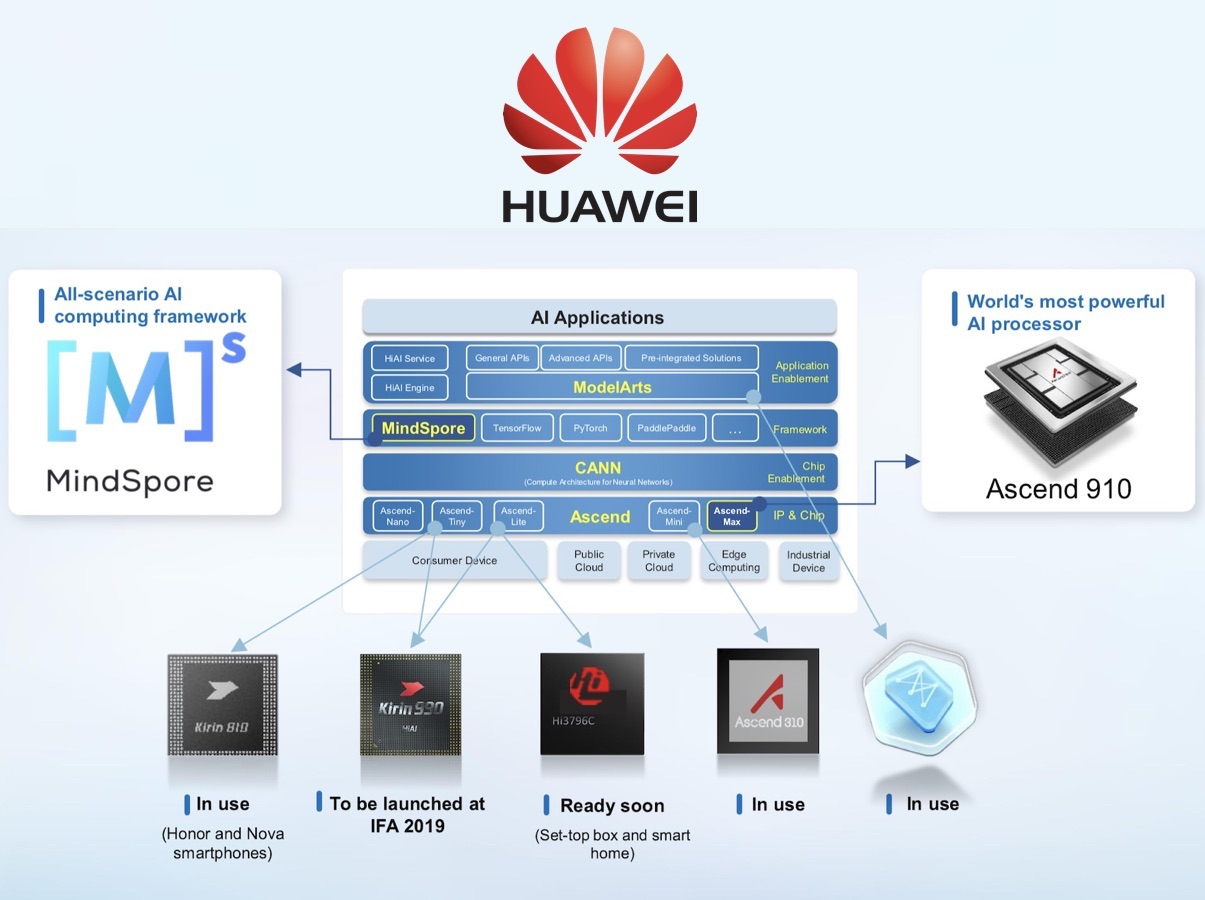
\includegraphics[width=0.7\textwidth]{images/figures/huaweiAIecosystem.jpg}
    \caption{Huawei AI Ecosystem}
    \label{fig: Huawei AI Ecosystem}
\end{figure}

% ── 2.3.1 ────────────────────────────────────────────────────
\subsection{Ascend Hardware Architecture}
\label{subsec:ascend-hw}

\subsubsection{DaVinci Core Architecture}

Huawei Ascend \acrshort{npu}s implement the DaVinci architecture, a
3D computational design consisting of three specialised processing units
per core:

\begin{table}[htbp]
  \centering
  \caption{DaVinci core computational units}
  \label{tab:davinci-units}
  \begin{tabularx}{\textwidth}{llXX}
    \toprule
    \tableheader{Unit & Dimensionality & Function & Operations/Cycle} \\
    \midrule
    Cube Unit   & 3D ($16\times16\times16$) & Matrix multiply-accumulate & 4,096 FP16 MACs + 8,192 INT8 MACs \\
    \rowcolor{TableRowOdd}
    Vector Unit & 2D (2,048-bit)            & Activation functions, element-wise & 2,048-bit INT8/FP16/FP32 \\
    Scalar Unit & 1D                        & Control flow, address generation   & Full flexibility, branch logic \\
    \bottomrule
  \end{tabularx}
\end{table}

The Cube Unit performs the fundamental 3D matrix operation
$D = A \times B + C$ where $A$, $B$, $C$, $D$ are all $16 \times 16$
matrices, yielding 4,096 parallel FP16 MAC operations in a single cycle.
The Vector Unit handles 2,048-bit wide activation and normalisation operations.
The Scalar Unit manages control flow and address generation, enabling the
Cube and Vector units to operate in pure dataflow mode.

\subsubsection{Ascend 910 Chip Specifications}

\begin{table}[htbp]
  \centering
  \caption{Huawei Ascend 910 key specifications}
  \label{tab:ascend-910-specs}
  \begin{tabularx}{0.9\textwidth}{lX}
    \toprule
    \tableheader{Parameter & Specification} \\
    \midrule
    AI Cores           & 32 DaVinci cores \\
    \rowcolor{TableRowOdd}
    FP16 Performance   & 256 TFLOPS/s @ 1.0 GHz \\
    INT8 Performance   & 512 TOPS \\
    \rowcolor{TableRowOdd}
    On-Chip SRAM       & 84 MB total (32 MB shared buffer) \\
    Memory             & 32 GB HBM2 via 4 channels \\
    \rowcolor{TableRowOdd}
    Memory Bandwidth   & 1,228 GB/s off-die \\
    Process Node       & 7nm+ EUV \\
    \rowcolor{TableRowOdd}
    TDP                & 300–350 W \\
    Interconnects      & PCIe 3.0 $\times$16, HCCS, 100G RoCE \\
    \bottomrule
  \end{tabularx}
\end{table}

The 32 DaVinci cores are organised in a mesh topology connected by the
CHIE Network-on-Chip (NOC). Each core has independent L0 buffers
(64 KB A + 64 KB B + 256 KB Unified), a 1 MB L1 buffer, and shares a
32 MB global buffer across all cores. Memory transfers between levels
are managed by the dedicated Memory Transfer Engine (\acrshort{mte}).


% ── 2.3.2 ────────────────────────────────────────────────────
\subsection{CANN Runtime Architecture}
\label{subsec:cann}

\acrfull{cann} is Huawei's heterogeneous computing architecture providing
the runtime, compiler, and operator library layer between AI frameworks
and Ascend hardware — the direct analogue of NVIDIA's \acrshort{cuda}
stack.

\begin{figure}[H]
    \centering
    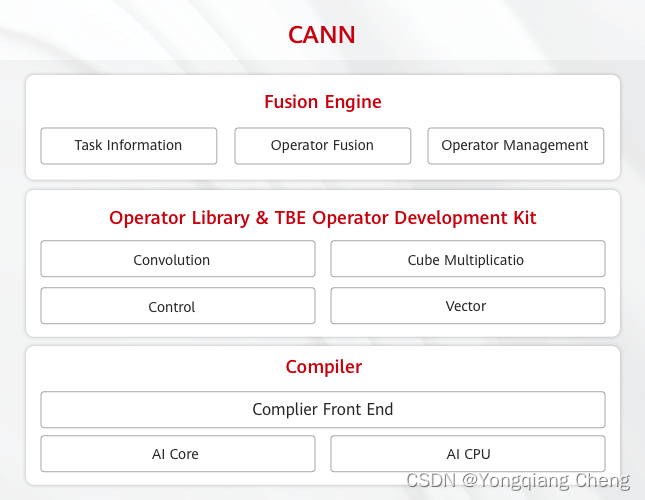
\includegraphics[width=0.7\textwidth]{images/figures/CANN-architecture.png}
    \caption{CANN Architecture Overview}
    \label{fig: CANN Architecture Overview}
\end{figure}

\subsubsection{Layered Architecture}

CANN is organised into two abstraction layers. \textbf{L1 (CANN)} is
the architecture-dependent layer providing hardware abstraction, task
scheduling, and the AscendCL API. \textbf{L2 (Graph Engine)} is
the architecture-independent optimisation layer performing operator
fusion, cross-layer memory optimisation, and compute-communication
parallelism.

AscendCL (Ascend Computing Language) is the unified programming interface
analogous to CUDA's runtime API, covering device and context management,
host-device memory transfers, model loading (from compiled \texttt{.om}
files), and stream-based asynchronous execution.

\subsubsection{Compiler Stack}

\begin{table}[htbp]
  \centering
  \caption{CANN compiler stack components}
  \label{tab:cann-compiler}
  \begin{tabularx}{\textwidth}{llX}
    \toprule
    \tableheader{Component & Input → Output & Function} \\
    \midrule
    Graph Compiler & IR → Hardware executable & Converts framework IR to Ascend executable \\
    \rowcolor{TableRowOdd}
    TBE (Tensor Boost Engine) & Operator → kernel & Auto-schedules efficient operator compilation \\
    OMG (Offline Model Generator) & Framework model → \texttt{.om} & Converts Caffe/TF/MindSpore to DaVinci offline model \\
    \bottomrule
  \end{tabularx}
\end{table}



% ── 2.3.3 ────────────────────────────────────────────────────
\subsection{MindSpore Execution Framework}
\label{subsec:mindspore}

MindSpore is Huawei's all-scenario AI framework supporting device-edge-cloud
deployment. It employs Source Code Transformation (\acrshort{sct}) for
automatic differentiation:
\begin{equation}
  \text{Function} \xrightarrow{\text{SCT}} \text{IR}
  \xrightarrow{\text{Parse}} \text{Computational Graph}
  \label{eq:sct}
\end{equation}

MindSpore offers a unified graph mode that switches seamlessly between
static execution (pre-compiled, production-optimised) and dynamic execution
(immediate, research-friendly) — a design advantage over PyTorch's separation
between eager and TorchScript modes.

In distributed training, MindSpore supports three parallel strategies
(data, model, hybrid) with an automatic parallelism search that explores
a large strategy space — contrasting with PyTorch's manual
\texttt{DistributedDataParallel} configuration.

\subsubsection{Performance}

The MindSpore + Ascend 910 combination achieves 1,802 images/second on
ResNet-50 V1.5 (ImageNet 2012) — approximately $2\times$ the throughput
of the mainstream TensorFlow + GPU baseline (965 img/s). This performance
advantage stems from MindSpore's native CANN integration eliminating the
translation overhead that external frameworks incur.


% ── 2.3.5 ────────────────────────────────────────────────────
\subsection{Ascend AI System Stack: End-to-End Integration}
\label{subsec:ascend-stack}

The four layers of the Ascend stack form a cohesive execution path from
user-facing AI code to hardware compute:

\begin{table}[htbp]
  \centering
  \caption{Full Ascend AI system stack}
  \label{tab:ascend-stack}
  \begin{tabularx}{\textwidth}{llX}
    \toprule
    \tableheader{Layer & Component & Primary Function} \\
    \midrule
    L4 & ModelArts      & AI lifecycle management, distributed training orchestration, MLOps \\
    \rowcolor{TableRowOdd}
    L3 & MindSpore      & Computational graph execution, automatic differentiation, parallelism \\
    L2 & CANN           & Graph optimisation, operator fusion, hardware abstraction, AscendCL API \\
    \rowcolor{TableRowOdd}
    L1 & Ascend (DaVinci) & Tensor computation via Cube/Vector/Scalar units \\
    \bottomrule
  \end{tabularx}
\end{table}

An important engineering caveat: MindSpore-native models achieve
$\approx 2\times$ the throughput of PyTorch/TensorFlow running on Ascend
via CANN, which incurs 10–20\% translation overhead. For production
systems targeting Ascend hardware, the native MindSpore path is strongly
preferred; frameworks migrated from the CUDA ecosystem must weigh this
performance cost against the effort of framework-level code changes.

% ============================================================
%  sec-4-software-stack.tex  —  2.4 AI Software Tools,
%  Frameworks and Infrastructure Stack
% ============================================================

\section{AI Software Tools, Frameworks, and Infrastructure Stack}
\label{sec:software-stack}

AI production systems are implemented as layered software stacks that
separate model development, distributed training, optimisation,
inference serving, orchestration, and infrastructure execution.
In a \acrshort{gpu}-to-\acrshort{npu} migration context, this stack
defines where model code remains portable and where vendor-specific
components introduce conversion, optimisation, and runtime dependencies.

The AI computing landscape is characterised by a fundamental asymmetry:
while low-level infrastructure (Docker, Kubernetes) and MLOps tooling
(W\&B, MLflow) are largely hardware-agnostic, the performance-critical
layers of model development and compilation are tightly coupled to
vendor-specific ecosystems. Table \ref{tab:full-stack} provides a mapping
of equivalent tools across the NVIDIA and Huawei stacks and their
portability.

\begin{table}[htbp]
  \centering
  \caption{Complete AI software and infrastructure stack portability overview}
  \label{tab:full-stack}
  \begin{tabularx}{\textwidth}{lXXl}
    \toprule
    \tableheader{Layer & NVIDIA Stack & Huawei Stack & Portability} \\
    \midrule
    Model dev.
      & PyTorch, HF Transformers, Megatron, DeepSpeed
      & MindSpore, MindFormers
      & Low \\
    \rowcolor{TableRowOdd}
    Distributed training
      & NCCL, DDP, FSDP
      & HCCL, MindSpore dist.
      & Medium \\
    Optimisation
      & TensorRT, TensorRT-LLM, CUDA Graphs
      & CANN, ATC, ACL
      & None \\
    \rowcolor{TableRowOdd}
    Inference serving
      & vLLM, Triton, NIM
      & MindSpore Serving, ModelArts
      & Low \\
    MLOps / tracking
      & W\&B, MLflow, Slurm, Ray
      & W\&B, MLflow, ModelArts
      & High \\
    \rowcolor{TableRowOdd}
    Infrastructure
      & Docker, Kubernetes, GitHub Actions
      & Docker, Kubernetes, GitHub Actions
      & Full \\
    \bottomrule
  \end{tabularx}
\end{table}

The infrastructure layer defines how AI workloads are executed across
local, cloud, and cluster environments. Containerisation via Docker and
orchestration via Slurm or Kubernetes ensure that the environment remains
consistent, which is critical for preserving reproducibility during
cross-hardware migration studies. Environment drift is a primary source
of performance loss, making clean infrastructure abstraction a prerequisite
for any successful migration project.




\blankpage
% ============================================================
%  chapters/03-nemotron-case-study/chapter.tex
%  Chapter 3 — State of the Art: Nemotron 3 Nano Case Study
% ============================================================

\chapter{State of the Art: Nemotron 3 Nano Case Study}
\label{chap:nemotron-case-study}

% ============================================================
%  sec-1-overview.tex  —  3.1 Nemotron 3 Nano Overview
% ============================================================

\section{Nemotron 3 Nano Overview}
\label{sec:nemotron-overview}

Nemotron 3 Nano is an open, efficient large language model developed by
NVIDIA and released in 2025. It belongs to the Nemotron 3 model family —
a suite of models spanning multiple capability tiers — and is positioned
as a high-efficiency alternative to models with significantly larger active
parameter counts. According to the repository root \texttt{README.md},
Nemotron 3 Nano \textit{``achieves better or on-par accuracy than competitive
models while having up to 3.3$\times$ higher inference throughput''} compared
to models such as GPT-OSS-20B and Qwen3-30B-A3B.

The model is designed for \textbf{agentic reasoning} workloads: multi-step,
multi-turn tasks requiring tool invocation, long-context comprehension, and
structured output generation. Its primary use cases, as documented in the
repository, include agentic pipelines with tool calling, extended context
document analysis (up to 1M tokens), multilingual tasks across 15+ languages,
and reasoning tasks with on/off reasoning-mode control.

% ── 3.1.1 ────────────────────────────────────────────────────
\subsection{Architecture}
\label{subsec:nemotron-architecture}

Nemotron 3 Nano implements a \term{Hybrid Mamba-Transformer} architecture
combined with a \term{sparse Mixture-of-Experts} (\acrshort{moe}) design.
This constitutes a departure from dense transformer-only architectures:
the hybrid design interleaves Mamba state-space model layers with standard
transformer attention layers, enabling efficient long-sequence processing
without the quadratic complexity of full self-attention across all layers.

The sparse \acrshort{moe} component activates only a subset of expert
networks per token during each forward pass, decoupling total parameter
count from per-token compute cost. \tabref{nemotron-arch-specs} documents
the architectural parameters extracted from the repository
\texttt{README.md}.

\begin{table}[htbp]
  \centering
  \caption{Nemotron 3 Nano architectural specifications}
  \label{tab:nemotron-arch-specs}
  \begin{tabularx}{0.88\textwidth}{lX}
    \toprule
    \tableheader{Parameter & Value} \\
    \midrule
    Total parameters         & 31.6B \\
    \rowcolor{TableRowOdd}
    Active parameters        & 3.6B (per forward pass) \\
    Architecture type        & Hybrid Mamba-Transformer with sparse MoE \\
    \rowcolor{TableRowOdd}
    Number of layers         & 32 \\
    Model dimension          & 3,008 \\
    \rowcolor{TableRowOdd}
    Total routable experts   & 128 \\
    Activated experts        & 6 per token per MoE layer \\
    \rowcolor{TableRowOdd}
    Shared experts           & 2 \\
    Pretraining tokens       & 25 trillion \\
    \rowcolor{TableRowOdd}
    Context length           & Up to 1M tokens \\
    Training stages          & 3 (Pretrain $\to$ SFT $\to$ RL) \\
    \bottomrule
  \end{tabularx}
\end{table}

The 31.6B/3.6B parameter ratio means that each forward pass activates
approximately 11.4\% of the total parameters. This is the efficiency
mechanism that enables inference throughput 3.3$\times$ higher than dense
models of similar capability.

% ── 3.1.2 ────────────────────────────────────────────────────
\subsection{Model Capabilities}
\label{subsec:nemotron-capabilities}

The following capabilities are documented in the repository
\texttt{README.md} and constitute the target requirements for the full
training pipeline described in subsequent sections.

% ── 3.1.3 ────────────────────────────────────────────────────
\subsection{Model Family Positioning}
\label{subsec:model-family}

The Nemotron 3 family, as referenced in the repository, comprises three
tiers: \textbf{Nano} (31.6B total / 3.6B active, optimised for throughput
and edge/cloud inference), \textbf{Super} (mid-tier capability/cost
balance), and \textbf{Ultra} (maximum capability, targeting frontier
benchmark performance). Nano's design rationale is explicit in the
repository: it trades total parameter count for inference efficiency by
exploiting sparse expert activation, making it deployable on hardware
configurations that cannot sustain dense models of equivalent benchmark
performance. The training pipeline — documented across four stage
directories — is shared in architecture across the family, with
stage-specific configurations controlling model dimension and parallelism
settings per tier.

% ============================================================
%  sec-2-training-lifecycle.tex  —  3.2 Training Lifecycle
% ============================================================

\section{Complete Nemotron Training Lifecycle}
\label{sec:training-lifecycle}

The Nemotron 3 Nano training pipeline is structured as a sequential
three-stage process documented across four directories in the repository:
\filepath{stage0\_pretrain/}, \filepath{stage1\_sft/}, \filepath{stage2\_rl/},
and \filepath{stage3\_eval/}. Each stage consumes the checkpoint artifact
produced by the previous stage, forming a lineage chain tracked through
Weights \& Biases artifacts. The complete pipeline flow is illustrated
in \figref{pipeline-overview}.

% ── Figure 3.2 placeholder ───────────────────────────────────
\begin{figure}[H]
    \centering
    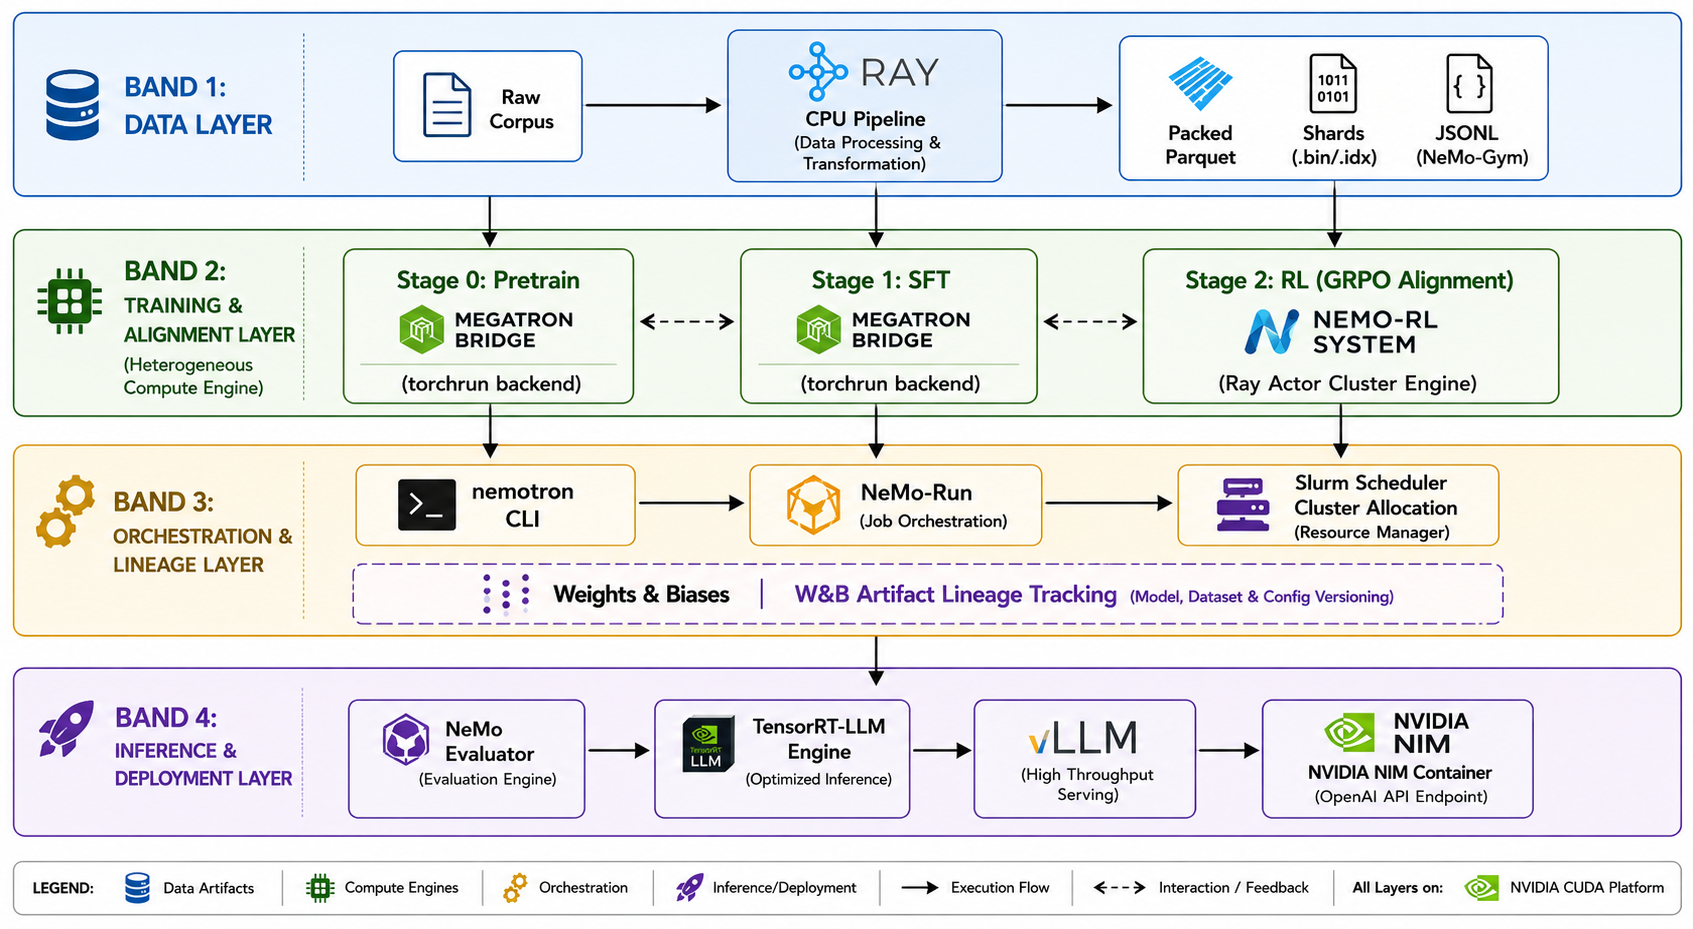
\includegraphics[width=0.85\textwidth]{images/figures/end2endnemopipeline.png}
    \caption{End-to-End Nemotron AI training pipeline Overview}
    \label{fig:pipeline-overview}
\end{figure}

% ── 3.2.1 ────────────────────────────────────────────────────
\subsection{Data Preparation}
\label{subsec:data-prep}

\subsubsection{Pretraining Data Preparation}
\label{subsubsec:pretrain-data-prep}

The pretraining data pipeline is implemented in
\filepath{stage0\_pretrain/data\_prep.py}. Its purpose is to tokenize raw
text corpora into Megatron's binary format (\texttt{.bin}/\texttt{.idx})
required by Megatron-Bridge's data loader.

The pipeline executes three sequential stages managed by the
\texttt{cosmos\_xenna.pipelines.v1} framework:

\begin{enumerate}
  \item \textbf{PlanStage}: Reads the dataset blend definition from
        \filepath{config/data\_prep/data\_blend\_raw.json}, performs
        deterministic work-item hashing, and generates per-shard
        \texttt{DatasetWorkItem} objects.
  \item \textbf{DownloadStage}: Fetches each dataset shard from its
        source (Hugging Face Hub or local storage), one node per shard.
  \item \textbf{BinIdxTokenizationStage}: Tokenizes documents using the
         tokenizer
        (\texttt{add\_bos=False}, \texttt{add\_eos=True}) and writes
        \texttt{.bin}/\texttt{.idx} file pairs.
\end{enumerate}

\begin{table}[htbp]
  \centering
  \caption{Pretraining data preparation: inputs, outputs, and configuration}
  \label{tab:pretrain-data-prep}
  \begin{tabularx}{\textwidth}{>{\hsize=0.6\hsize}L >{\hsize=1.4\hsize}L}
    \toprule
    \tableheader{Property & Detail} \\
    \midrule
    Entry point    & \texttt{stage0\_pretrain/data\_prep.py} \\
    \rowcolor{TableRowOdd}
    Input format   & Raw text datasets (HF Hub or local); blend defined in
                     \texttt{config/data\_prep/data\_blend\_raw.json} \\
    Output format  & Megatron \texttt{.bin}/\texttt{.idx} shards +
                     \texttt{blend.json} per-split index \\
    \rowcolor{TableRowOdd}
    Sharding       & 128 output shards by default (1 if \texttt{sample} mode) \\
    Tokenizer      & \path{nvidia/NVIDIA-Nemotron-Nano-9B-v2};
                     \texttt{add\_bos=False}, \texttt{add\_eos=True} \\
    \rowcolor{TableRowOdd}
    Split output   & \texttt{blend.json}:
                     \texttt{\{"train": [...], "valid": [...], "test": [...]\}} \\
    W\&B artifact  & \texttt{PretrainBlendsArtifact} (\texttt{nano3-pretrain-data}) \\
    \rowcolor{TableRowOdd}
    Execution mode & Ray (CPU-only nodes, \texttt{gpus\_per\_node=0}) \\
    \bottomrule
  \end{tabularx}
\end{table}

\subsubsection{SFT Data Preparation}
\label{subsubsec:sft-data-prep}

The SFT data pipeline (\filepath{stage1\_sft/data\_prep.py}) processes
OpenAI-format chat datasets into packed Parquet shards with role-based loss
masking. The pipeline applies four transformations in sequence:

\begin{enumerate}
  \item \textbf{Chat template application}: The \texttt{nano3} chat
        template is applied to \texttt{messages} fields, producing
        role-labelled token chunks (system, user, assistant).
  \item \textbf{Tokenisation with loss masking}: \texttt{input\_ids}
        are generated with a \texttt{loss\_mask} array where system and
        user tokens are masked to 0 and assistant tokens are set to 1,
        ensuring the model only learns to predict assistant responses.
  \item \textbf{Sequence packing}: Sequences are packed up to
        \texttt{pack\_size=4096} tokens using the
        \texttt{first\_fit\_shuffle} algorithm to maximise GPU utilisation
        during training.
  \item \textbf{Parquet serialisation}: Packed sequences are written
        as \texttt{zstd}-compressed Parquet shards with row group size
        1,000, compatible with Megatron-Bridge's
        \texttt{FinetuningDatasetConfig}.
\end{enumerate}

\begin{table}[htbp]
  \centering
  \caption{SFT data preparation: inputs, outputs, and key parameters}
  \label{tab:sft-data-prep}
  \begin{tabularx}{\textwidth}{>{\hsize=0.6\hsize}L >{\hsize=1.4\hsize}L}
    \toprule
    \tableheader{Property & Detail} \\
    \midrule
    Entry point      & \texttt{stage1\_sft/data\_prep.py} \\
    \rowcolor{TableRowOdd}
    Input format     & OpenAI chat format: \texttt{\{"messages": [\{"role", "content"\}]\}} \\
    Output format    & Packed Parquet shards; canonical split directories via symlinks \\
    \rowcolor{TableRowOdd}
    Loss mask        & \texttt{loss\_mask=0} for system/user; \texttt{loss\_mask=1} for assistant \\
    Pack size        & 4,096 tokens per packed sequence \\
    \rowcolor{TableRowOdd}
    Split ratios     & \texttt{train=0.98}, \texttt{valid=0.01}, \texttt{test=0.01} \\
    W\&B artifact    & \texttt{SFTDataArtifact} (\texttt{nano3/sft/data}) \\
    \rowcolor{TableRowOdd}
    Execution mode   & Ray (CPU-only nodes, \texttt{gpus\_per\_node=0}) \\
    \bottomrule
  \end{tabularx}
\end{table}

\subsubsection{RL Data Preparation}
\label{subsubsec:rl-data-prep}

The RL data pipeline (\filepath{stage2\_rl/data\_prep.py}) converts
preference datasets into JSONL format for consumption by NeMo-RL's
NeMo-Gym interface. The \texttt{nemotron\_rl} transform extracts prompts
from \texttt{responses\_create\_params.input} fields. Output is written
to three split directories: \texttt{train/data.jsonl},
\texttt{val/data.jsonl}, \texttt{test/data.jsonl}, with a
\texttt{manifest.json} tracking split paths and ratios.

% ── 3.2.2 ────────────────────────────────────────────────────
\subsection{Pretraining Pipeline}
\label{subsec:pretrain-pipeline}

\subsubsection{Execution Architecture}

The pretraining stage is implemented in \filepath{stage0\_pretrain/train.py}
and uses Megatron-Bridge as the distributed training framework. The script
is launched via \texttt{torchrun} across 2 nodes with 8 GPUs each (16 GPUs
total). The configuration system uses OmegaConf YAML files with
Hydra-style \texttt{key=value} CLI overrides, with two configurations
provided in \tabref{pretrain-configs}.

\begin{table}[htbp]
  \centering
  \caption{Pretraining configuration files}
  \label{tab:pretrain-configs}
  \begin{tabularx}{\textwidth}{>{\hsize=0.8\hsize}L >{\hsize=0.8\hsize}L >{\hsize=1.4\hsize}L}
    \toprule
    \tableheader{File & Purpose & Key Parameters} \\
    \midrule
    \texttt{config/default.yaml}
      & Production
      & Recipe: \texttt{nemotron\_3\_nano\_pretrain\_config};
        data from \texttt{nano3-pretrain-data:latest} artifact;
        checkpoint saved to \texttt{/nemo\_run/nano3-pretrain-model} \\
    \rowcolor{TableRowOdd}
    \texttt{config/tiny.yaml}
      & Testing
      & Recipe: \texttt{qwen3\_8b\_pretrain\_config};
        \texttt{train\_iters=1700}; \texttt{global\_batch\_size=32};
        \texttt{lr\_warmup\_iters=32} \\
    \bottomrule
  \end{tabularx}
\end{table}


% ── 3.2.3 ────────────────────────────────────────────────────
\subsection{Supervised Fine-Tuning Pipeline}
\label{subsec:sft-pipeline}

\subsubsection{Training Architecture}

The SFT stage (\filepath{stage1\_sft/train.py}) uses Megatron-Bridge's
\texttt{finetune()} function in place of \texttt{pretrain()}, with a
\texttt{FinetuningDatasetConfig} built directly from packed Parquet shards
rather than via the standard Hugging Face dataset loading path. This
distinction is critical: the \texttt{\_build\_dataset\_config()} function
in \texttt{stage1\_sft/train.py} constructs a \texttt{FinetuningDatasetConfig}
with \texttt{PackedSequenceSpecs} pointing to the canonical split directories
produced by data preparation, explicitly bypassing \texttt{HFDatasetConfig}
to avoid unnecessary dataset downloads.

\subsubsection{Model Parallelism Configuration}

The production configuration specifies a four-way tensor parallelism layout
(\texttt{tensor\_model\_parallel\_size: 4}) with a hidden size of 1,344.

\begin{table}[htbp]
  \centering
  \caption{SFT stage artifact inputs and outputs (Nemotron Baseline)}
  \label{tab:nemotron-sft-artifacts}
  \begin{tabularx}{\textwidth}{>{\hsize=0.6\hsize}L >{\hsize=1.0\hsize}L >{\hsize=1.4\hsize}L}
    \toprule
    \tableheader{Direction & Artifact & Description} \\
    \midrule
    Input (model) & \path{nano3-pretrain-model:latest}
      & Pretrained Megatron checkpoint; \texttt{finetune: true} skips
        optimizer state loading \\
    \rowcolor{TableRowOdd}
    Input (data)  & \path{nano3-sft-data:latest}
      & Packed Parquet shards + canonical split directories \\
    Output        & \path{nano3-sft-model:latest}
      & Fine-tuned Megatron checkpoint; saved every 20 iterations \\
    \bottomrule
  \end{tabularx}
\end{table}

% ── 3.2.4 ────────────────────────────────────────────────────
\subsection{Reinforcement Learning Pipeline}
\label{subsec:rl-pipeline}


\subsubsection{Checkpoint Initialisation}

The RL stage handles two distinct checkpoint initialisation paths:
(1) \textbf{HF conversion path}: the SFT Megatron checkpoint is
converted to HuggingFace format via
\texttt{megatron.bridge.AutoBridge.export\_ckpt()}, enabling vLLM to
load the fine-tuned weights directly for generation; (2)
\textbf{fake step-0 path}: a \texttt{step\_0/policy/weights/} directory
structure is created by symlinking the Megatron checkpoint, allowing
NeMo-RL's checkpointer to resume from it while vLLM continues using
the base HF model for generation.

\subsubsection{NeMo-Gym Environment Integration}

NeMo-Gym provides the reward computation infrastructure. The
\texttt{NemoGym} Ray actor is initialised with a
\texttt{NemoGymConfig} containing the model name, vLLM server base URLs,
and environment-specific configuration. A blocking \texttt{health\_check}
call ensures the actor is ready before training begins. The
\texttt{task\_to\_env} mapping associates training tasks with their
corresponding reward environments.

\begin{table}[htbp]
  \centering
  \caption{RL stage key components and their roles}
  \label{tab:rl-components}
  \begin{tabularx}{\textwidth}{>{\hsize=0.7\hsize}L >{\hsize=0.5\hsize}L >{\hsize=1.8\hsize}L}
    \toprule
    \tableheader{Component & Type & Role in Pipeline} \\
    \midrule
    \texttt{grpo\_train()} & NeMo-RL function & Main training loop \\
    \rowcolor{TableRowOdd}
    \texttt{NemoGym} & Ray actor & Reward environment server \\
    \texttt{policy\_generation} & vLLM actor & Response generation \\
    \rowcolor{TableRowOdd}
    \texttt{policy} & Megatron model & Weight update (gradient computation) \\
    \texttt{checkpointer} & NeMo-RL utility & Step-based checkpoint saving \\
    \rowcolor{TableRowOdd}
    \texttt{HCCL} / \texttt{NCCL} & Collective comm. & Gradient synchronisation \\
    \bottomrule
  \end{tabularx}
\end{table}

\begin{table}[htbp]
  \centering
  \caption{RL stage artifact inputs and outputs}
  \label{tab:rl-artifacts}
  \begin{tabularx}{\textwidth}{>{\hsize=0.6\hsize}L >{\hsize=1.0\hsize}L >{\hsize=1.4\hsize}L}
    \toprule
    \tableheader{Direction & Artifact & Description} \\
    \midrule
    Input (model) & \texttt{nano3-sft-model:latest}
      & SFT checkpoint; converted to HF format or symlinked as step-0 \\
    \rowcolor{TableRowOdd}
    Input (data)  & \texttt{nano3-rl-data:latest}
      & JSONL files: \texttt{train/data.jsonl}, \texttt{val/data.jsonl} \\
    Output        & \texttt{nano3-rl-model}
      & Aligned model checkpoint; step-based saves via NeMo-RL checkpointer \\
    \bottomrule
  \end{tabularx}
\end{table}

% ── 3.2.5 ────────────────────────────────────────────────────
\subsection{Evaluation Pipeline}
\label{subsec:eval-pipeline}

The evaluation stage resides in \filepath{stage3\_eval/} and uses the
NeMo Evaluator framework. Evaluation is configured via YAML benchmark
configuration files that specify the target model artifact
(\texttt{ModelArtifact-rl:latest}), benchmark suites, and metric
collection parameters. The NeMo Evaluator deploys the model as an
inference service, submits benchmark prompts, collects model outputs,
and aggregates metrics.

% ── 3.2.6 ────────────────────────────────────────────────────
\subsection{Inference and Deployment}
\label{subsec:inference-deployment}

The repository root \texttt{README.md} and stage documentation reference
three deployment paths for the final aligned model:

\begin{table}[htbp]
  \centering
  \caption{Nemotron 3 Nano inference and deployment options}
  \label{tab:deployment-options}
  \begin{tabularx}{\textwidth}{>{\hsize=0.7\hsize}L >{\hsize=0.7\hsize}L >{\hsize=1.6\hsize}L}
    \toprule
    \tableheader{Engine & Role & Notes} \\
    \midrule
    TensorRT-LLM
      & Optimised inference
      & Model compiled to TRT engine; used in production NIM deployment \\
    \rowcolor{TableRowOdd}
    vLLM
      & Serving engine
      & Used during RL training for generation; also standalone serving path \\
    NVIDIA NIM
      & Enterprise deployment
      & Container-based; wraps TensorRT-LLM runtime with OpenAI API \\
    \bottomrule
  \end{tabularx}
\end{table}

During the RL stage, vLLM is used directly as the generation backend
within the \texttt{policy\_generation} actor, confirming tight integration
between the training and inference stacks.

% ============================================================
%  sec-3-technical-stack.tex  —  3.3 Technical Stack Analysis
% ============================================================

\section{Technical Stack Analysis}
\label{sec:technical-stack}

% ── 3.3.1 ────────────────────────────────────────────────────
\subsection{Megatron-Bridge}
\label{subsec:megatron-bridge}

Megatron-Bridge is the distributed training framework used in Stages 0
and 1. It acts as an abstraction layer over Megatron-LM, providing:
(1) a \texttt{ConfigContainer} dataclass for unified configuration of
model architecture, training loop, optimiser, scheduler, logging, and
checkpointing; (2) \texttt{pretrain()} and \texttt{finetune()} entry-point
functions that encapsulate the Megatron training loop; and (3) a recipe
system that maps named model architectures (e.g.,
\texttt{nemotron\_3\_nano\_pretrain\_config}) to fully-specified
\texttt{ConfigContainer} instances.

The \texttt{create\_omegaconf\_dict\_config()} utility converts the
Python dataclass to an OmegaConf \texttt{DictConfig}, enabling merging
of YAML file overrides and Hydra-style CLI overrides before converting
back to the final \texttt{ConfigContainer} via \texttt{apply\_overrides()}.

The \texttt{stage1\_sft/config/default.yaml} file mounts specific Git
commits of both Megatron-LM and Megatron-Bridge into the container at
\texttt{/opt/megatron-lm} and \texttt{/opt/Megatron-Bridge}, confirming
that production SFT uses pinned dependency versions rather than container
image defaults.

% ── 3.3.2 ────────────────────────────────────────────────────
\subsection{NeMo-RL}
\label{subsec:nemo-rl}

NeMo-RL is the reinforcement learning framework exclusive to Stage 2.
It provides the \texttt{grpo\_train()} function, the
\texttt{AllTaskProcessedDataset} data interface, the NeMo-Gym environment
integration layer, and the \texttt{VirtualCluster} Ray initialisation
utilities. Its container image (\path{nvcr.io/nvidia/nemo-rl:v0.4.0.nemotron_3_nano})
is distinct from the Megatron-Bridge NeMo container used in Stages 0
and 1, reflecting a separate dependency environment.

NeMo-RL's architecture within the RL stage involves four co-existing
Ray actor types: the \texttt{policy} actor (Megatron-Bridge-backed weight
update), the \texttt{policy\_generation} actor (vLLM-backed generation),
the \texttt{NemoGym} actor (reward computation), and the
\texttt{cluster} virtual cluster coordinator. This actor decomposition
allows generation and weight updates to proceed on separate GPU allocations
within the same Ray cluster.

% ── 3.3.3 ────────────────────────────────────────────────────
\subsection{CUDA Dependency Analysis}
\label{subsec:cuda-deps}

Every execution stage in the Nemotron 3 Nano pipeline has a direct
\acrshort{cuda} dependency. \tabref{cuda-deps} documents this per stage
based on repository evidence.

\begin{table}[htbp]
  \centering
  \caption{CUDA dependencies per execution stage}
  \label{tab:cuda-deps}
  \begin{tabularx}{\textwidth}{l X X}
    \toprule
    \tableheader{Stage & CUDA Dependency & Functional Role} \\
    \midrule
    Data Prep
      & None (CPU-only)
      & Ray-based document tokenisation \\
    \rowcolor{TableRowOdd}
    Pretraining
      & \texttt{selective\_scan\_cuda}, cuBLAS, NCCL
      & Fused SSM kernels, matmul, distributed training \\
    SFT
      & Megatron-Bridge, cuBLAS, NCCL
      & PyTorch-based fine-tuning acceleration \\
    \rowcolor{TableRowOdd}
    RL (GRPO)
      & vLLM, NeMo-RL, Ray, NCCL
      & High-throughput generation and weight updates \\
    Evaluation
      & lm-eval, PyTorch
      & Parallel accuracy benchmarking \\
    \rowcolor{TableRowOdd}
    Inference
      & TensorRT-LLM, vLLM, Triton
      & GPU-optimised model serving \\
    \bottomrule
  \end{tabularx}
\end{table}

% ── 3.3.4 ────────────────────────────────────────────────────
\subsection{Infrastructure Dependency Visualization}
\label{subsec:infra-viz}

The inter-dependency between the hardware, drivers, and frameworks is visualized in \figref{NVIDIA Infrastructure Dependency Diagram}.

\begin{figure}[H]
    \centering
    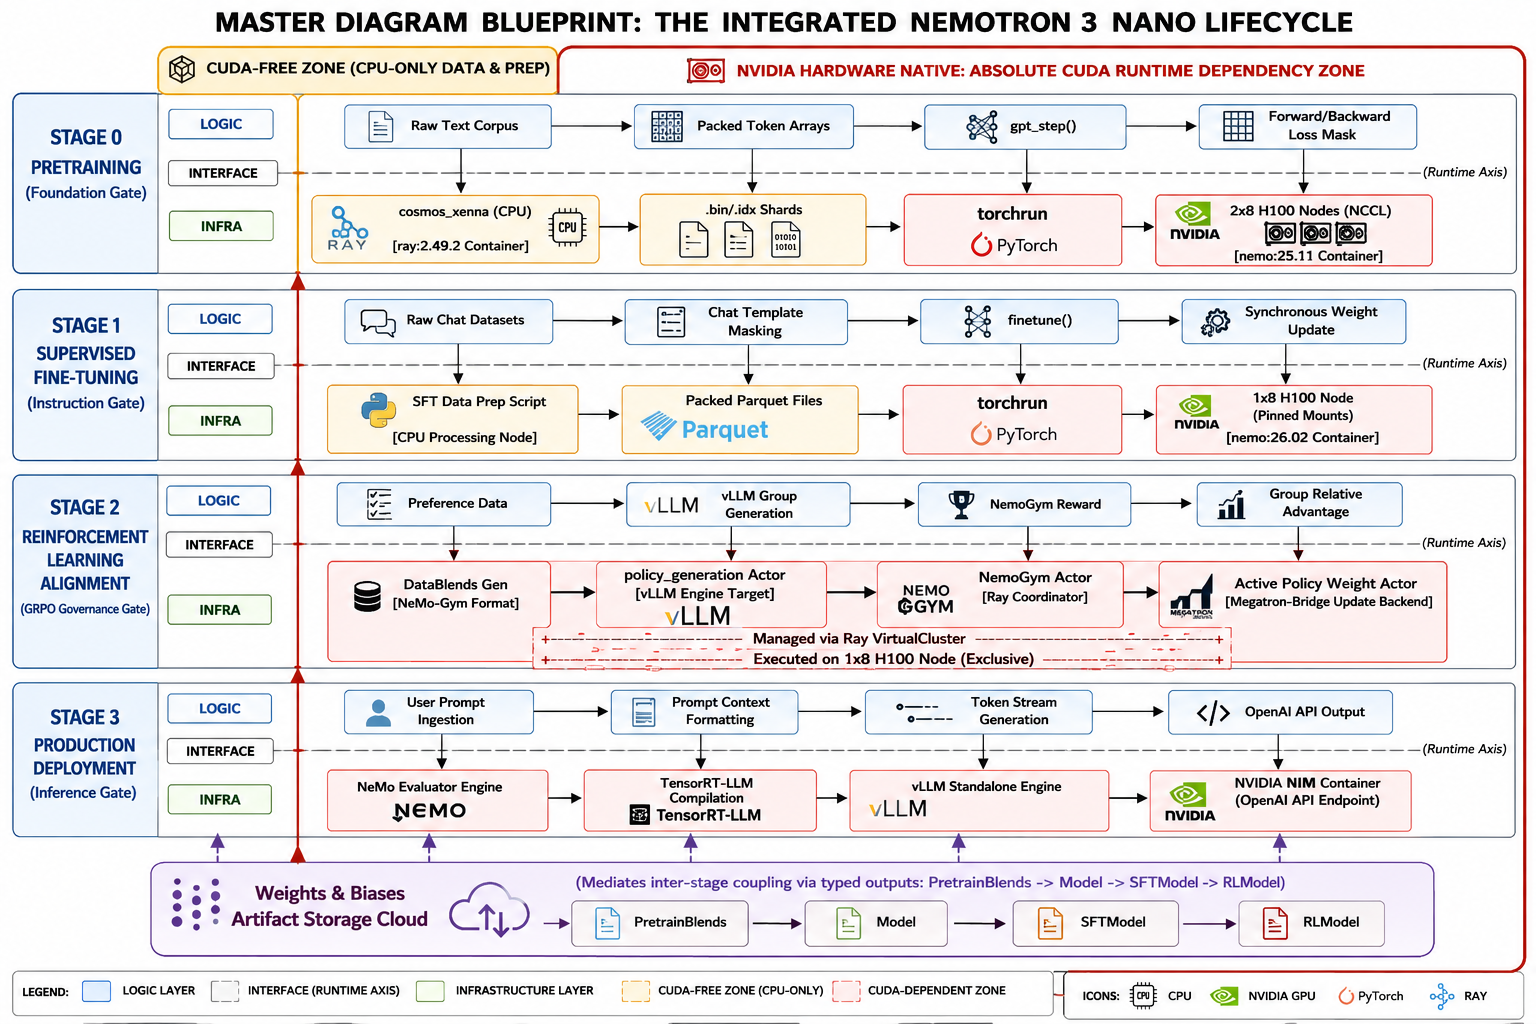
\includegraphics[width=0.85\textwidth]{images/figures/infra-dependecy-highlight.png}
    \caption{NVIDIA Infrastructure Dependency Diagram}
    \label{fig:NVIDIA Infrastructure Dependency Diagram}
\end{figure}



% ── 3.3.5 ────────────────────────────────────────────────────
\subsection{Experiment Tracking and Artifact Management}
\label{subsec:wandb-artifacts}

Weights \& Biases serves two distinct roles in the pipeline: experiment
tracking and artifact lineage management. W\&B is initialised in each
stage to capture training metrics, configuration snapshots, and
checkpoint logs, with several monkey-patches applied to ensure
compatibility with Megatron-Bridge. The pipeline also uses W\&B
artifacts as the inter-stage handoff mechanism, creating an unbroken
lineage graph from raw datasets to the final aligned model, as
documented in \tabref{artifact-lineage}.

\begin{table}[htbp]
  \centering
  \caption{W\&B artifact lineage across pipeline stages}
  \label{tab:artifact-lineage}
  \begin{tabularx}{\textwidth}{>{\hsize=0.7\hsize}L >{\hsize=1.0\hsize}L >{\hsize=1.0\hsize}L >{\hsize=1.3\hsize}L}
    \toprule
    \tableheader{Stage & Artifact In & Artifact Out & Type} \\
    \midrule
    Pretrain data prep
      & Raw datasets
      & \path{nano3-pretrain-data:latest}
      & \texttt{PretrainBlendsArtifact} \\
    \rowcolor{TableRowOdd}
    Pretraining
      & \path{nano3-pretrain-data:latest}
      & \path{nano3-pretrain-model:latest}
      & \texttt{ModelArtifact} \\
    SFT data prep
      & Raw chat datasets
      & \path{nano3-sft-data:latest}
      & \texttt{SFTDataArtifact} \\
    \rowcolor{TableRowOdd}
    SFT
      & \path{nano3-pretrain-model:latest} + \path{nano3-sft-data:latest}
      & \path{nano3-sft-model:latest}
      & \texttt{ModelArtifact} \\
    RL data prep
      & Raw preference datasets
      & \path{nano3-rl-data:latest}
      & \texttt{DataBlendsArtifact} \\
    \rowcolor{TableRowOdd}
    RL (GRPO)
      & \path{nano3-sft-model:latest} + \path{nano3-rl-data:latest}
      & \path{nano3-rl-model}
      & \texttt{ModelArtifact} \\
    \bottomrule
  \end{tabularx}
\end{table}

% ============================================================
%  sec-4-consolidated-architecture.tex  —  3.4 Consolidated Architecture
% ============================================================

\section{Consolidated Nemotron 3 Nano Architecture}
\label{sec:consolidated-architecture}

% ── 3.4.1 ────────────────────────────────────────────────────
\subsection{End-to-End Architecture Description}
\label{subsec:e2e-architecture}

The Nemotron 3 Nano training and deployment system constitutes a
vertically integrated NVIDIA-stack pipeline spanning data ingestion,
distributed training, alignment, evaluation, and production inference.
The architecture is characterised by three structural properties.

\textbf{Stage isolation with artifact-mediated handoff.} Each stage
is an independently deployable unit communicating exclusively through
W\&B artifacts.
\textbf{Framework heterogeneity across stages.} The pipeline uses
Megatron-Bridge, NeMo-RL, and cosmos\_xenna to address different
training semantics.
\textbf{Configuration-driven architecture selection.} The recipe system
enables swapping model architectures via a single configuration field
with no code changes.

% ── 3.4.2 ────────────────────────────────────────────────────
\subsection{Training Infrastructure Summary}
\label{subsec:training-infra-summary}

\begin{table}[htbp]
  \centering
  \caption{Training infrastructure summary by stage}
  \label{tab:training-summary}
  \begin{tabularx}{\textwidth}{>{\hsize=0.6\hsize}L >{\hsize=1.2\hsize}L l l l >{\hsize=1.4\hsize}L}
    \toprule
    \tableheader{Stage & Framework & Launch & Nodes & GPUs & Container} \\
    \midrule
    Data Prep
      & cosmos\_xenna + Ray
      & ray
      & 1
      & 0
      & \path{anyscale/ray:2.49.2-py312} \\
    \rowcolor{TableRowOdd}
    Pretrain
      & Megatron-Bridge
      & torchrun
      & 2
      & 8/node
      & \path{nemo:25.11.nemotron_3_nano} \\
    SFT
      & Megatron-Bridge
      & torchrun
      & 1
      & 8/node
      & \path{nemo:26.02.super.rc1} \\
    \rowcolor{TableRowOdd}
    RL (GRPO)
      & NeMo-RL + Ray
      & ray
      & 1
      & 8/node
      & \path{nemo-rl:v0.4.0.nemotron_3_nano} \\
    \bottomrule
  \end{tabularx}
\end{table}

% ── 3.4.3 ────────────────────────────────────────────────────
\subsection{Inference Infrastructure and Dependency Summary}
\label{subsec:inference-summary}

\begin{table}[htbp]
  \centering
  \caption{Inference infrastructure options}
  \label{tab:inference-summary}
  \begin{tabularx}{\textwidth}{>{\hsize=0.6\hsize}L >{\hsize=1.4\hsize}L >{\hsize=1.0\hsize}L}
    \toprule
    \tableheader{Engine & Integration Point & Deployment Context} \\
    \midrule
    vLLM
      & RL generation backend (\texttt{policy\_generation} actor); standalone serving
      & Research and production serving \\
    \rowcolor{TableRowOdd}
    TensorRT-LLM
      & Post-training compilation of final checkpoint
      & Optimised production inference \\
    NVIDIA NIM
      & Containerised packaging of TRT-LLM engine
      & Enterprise deployment; OpenAI-compatible API \\
    \rowcolor{TableRowOdd}
    NeMo Evaluator
      & Benchmark inference during Stage 3 evaluation
      & Accuracy measurement before deployment \\
    \bottomrule
  \end{tabularx}
\end{table}


% ── 3.4.5 ────────────────────────────────────────────────────
\subsection{Concluding Remarks}
\label{subsec:ch3-conclusion}

The Nemotron 3 Nano ecosystem implements a complete, production-grade
LLM lifecycle spanning pretraining, supervised fine-tuning, reinforcement
learning alignment, evaluation, and deployment. Each stage is implemented
as a discrete, independently executable unit communicating through typed
W\&B artifacts. The training stack is exclusively NVIDIA-native: every
GPU-accelerated stage depends on \acrshort{cuda}, cuDNN, NCCL, or
TensorRT-LLM with no hardware-agnostic abstraction layer between the
framework code and NVIDIA's accelerator stack. The data preparation
pipeline, operating on CPU-only Ray nodes, is the sole stage with no
direct \acrshort{cuda} dependency.

This architecture constitutes the reference NVIDIA-based ecosystem that
will be analysed and used as the baseline for the migration study
presented in the next chapter.



\blankpage
% ============================================================
%  chapters/04-migration-implementation/chapter.tex
%  Chapter 4 — CUDA-to-CANN Migration: Implementation
% ============================================================

\chapter{CUDA-to-CANN Migration: Implementation and Deployment}
\label{chap:migration-implementation}

% ============================================================
%  sec-1-usecase-dataset.tex  —  4.1 Use Case, Dataset, and
%  Project Structure
% ============================================================

\section{Use Case Definition and Dataset Construction}
\label{sec:usecase-dataset}


The migration target for this project is a concrete, industrially
grounded use case: a \term{Multilingual Technical Support Assistant}
for \acrshort{mena} Telecom Infrastructure. The system is designed
to assist enterprise clients of \CompanyName{} — telecom operators,
\acrshort{isp}s, and enterprise \acrshort{it} teams — in resolving
technical issues related to 5G infrastructure, Huawei network
equipment, optical transport networks, and enterprise \acrshort{it}
systems. Supported languages are English, Arabic, and French,
reflecting the linguistic profile of \CompanyName{}'s Northern Africa
customer base.

This use case was selected for three concrete reasons. First, Nemotron
3 Nano's native multilingual support (15+ languages) and 1M-token
context window align directly with the requirements of multi-document
technical queries and multi-turn support conversations. Second, the
3.6B active parameter count fits within the 64~GB \acrshort{hbm2}
of a single Ascend 910C, enabling single-node inference without
tensor parallelism. Third, the domain-specificity of technical support
provides clear, measurable evaluation criteria — keyword coverage,
command correctness, and language accuracy — rather than the
subjective metrics of general-purpose assistants.

The use case positions the fine-tuned model as the intelligence layer
of a production support platform, with the inference server exposing
an OpenAI-compatible \acrshort{rest} \acrshort{api} that can be
integrated into ticketing systems, chat interfaces, and
\acrshort{cli} tooling without modification.

\subsection{Dataset Blend}
\label{subsec:dataset}

The \acrshort{sft} dataset is constructed from four publicly
available HuggingFace datasets, blended by weight to reflect the
target language and domain distribution. \tabref{dataset-blend}
documents each source.

\begin{table}[htbp]
  \centering
  \caption{SFT dataset blend for the telecom support use case}
  \label{tab:dataset-blend}
  \begin{tabularx}{\textwidth}{P{3.5cm} L c P{2cm} r}
    \toprule
    \tableheader{Dataset & HuggingFace Path & Lang. & Size & Weight} \\
    \midrule
    Salesforce DialogStudio
      & \texttt{Salesforce/dialogstudio}
      & EN & $\sim$50K & 0.40 \\
    \rowcolor{TableRowOdd}
    Arabic Alpaca
      & \texttt{kunishou/ArabicAlpaca}
      & AR & $\sim$52K & 0.30 \\
    Open-Platypus
      & \texttt{garage-bAInd/Open-Platypus}
      & EN/FR & $\sim$25K & 0.20 \\
    \rowcolor{TableRowOdd}
    OPUS-100 (fr-ar)
      & \texttt{Helsinki-NLP/opus-100}
      & FR/AR & $\sim$10K & 0.10 \\
    \midrule
    \textbf{Total}
      & & & $\sim$137K & 1.00 \\
    \bottomrule
  \end{tabularx}
\end{table}

Each dataset undergoes a distinct formatting transformation
implemented in \filepath{data/prepare\_datasets.py}. The
\textbf{DialogStudio TechSupport} split contains multi-turn
technical support conversations in OpenAI dialog format; each
dialog is parsed by iterating over \texttt{roles} fields and
mapping \texttt{USR} tokens to \texttt{user} turns and \texttt{SYS}
tokens to \texttt{assistant} turns. The \textbf{Arabic Alpaca}
dataset uses an instruction-input-output structure; the
\texttt{instruction} and optional \texttt{input} fields are
concatenated into the \texttt{user} turn, and the \texttt{output}
becomes the \texttt{assistant} turn. The \textbf{Open-Platypus}
dataset is filtered to retain only samples containing technical
keywords (network, protocol, server, system, réseau, etc.) before
formatting. The \textbf{OPUS-100 fr-ar} translation pairs are
converted into synthetic bilingual QA samples where a French
technical sentence becomes the user query and the Arabic translation
becomes the assistant response, filtered to retain only
telecom-relevant vocabulary.

All samples are formatted to a unified OpenAI chat \acrshort{json}
schema with system, user, and assistant roles, as described in
Chapter 3.

Three language-specific system prompts are defined in
\filepath{data/prepare\_datasets.py} and injected based on
dataset source:

\begin{itemize}
  \item \texttt{SYSTEM\_PROMPT\_EN} — English prompt positioning the
        model as a Huawei telecom support specialist
  \item \texttt{SYSTEM\_PROMPT\_AR} — Arabic prompt with equivalent
        framing in \acrshort{msa}
  \item \texttt{SYSTEM\_PROMPT\_FR} — French prompt for
        French-language client interactions
\end{itemize}

During inference, the server automatically detects the language of
the incoming user query (via Unicode Arabic character ratio and
French lexical markers) and injects the appropriate system prompt,
ensuring consistent role framing without requiring the client
application to supply a system prompt.

\subsection{Dataset Preparation Pipeline}
\label{sec:data-prep-pipeline}

The dataset preparation executes in two stages. In the first stage, raw
datasets are downloaded and formatted to \texttt{.jsonl} using
\filepath{data/prepare\_datasets.py}.

The second stage runs the Nemotron SFT data pipeline on the formatted
files to apply the chat template and produce packed Parquet shards.

% ============================================================
%  sec-2-architecture-strategy.tex  —  4.2 Architecture and
%  Migration Strategy
% ============================================================

\section{Architecture and Migration Strategy}
\label{sec:architecture-strategy}

\subsection{Full Stack Migration Overview}
\label{subsec:stack-overview}

The migration replaces every \acrshort{cuda}-dependent component in
the Nemotron 3 Nano pipeline with a CANN-compatible equivalent,
while preserving the components that are hardware-agnostic. \tabref{full-stack-mapping}
documents the complete mapping.

\newcolumntype{K}{>{\raggedright\arraybackslash\ttfamily\scriptsize}X} % Use scriptsize for very long code names in tables

\begin{table}[htbp]
  \centering
  \caption{Complete CUDA-to-CANN stack mapping}
  \label{tab:full-stack-mapping}
  \begin{tabularx}{\textwidth}{l K K l}
    \toprule
    \tableheader{Layer & CUDA (Original) & CANN (Target) & Change} \\
    \midrule
    Hardware
      & NVIDIA H100 SXM5
      & Huawei Ascend 910C
      & Infrastructure \\
    \rowcolor{TableRowOdd}
    Compute runtime
      & CUDA + cuDNN + cuBLAS
      & CANN AscendCL + CANN NN Library
      & Abstracted via \texttt{torch\_npu} \\
    Distributed comm.
      & NCCL
      & HCCL
      & Backend string change \\
    \rowcolor{TableRowOdd}
    Training framework
      & Megatron-Bridge + \texttt{torchrun}
      & Megatron-Bridge + \texttt{torch\_npu} + \texttt{torchrun}
      & Patched entry point \\
    Mamba SSM kernel
      & \texttt{selective\_scan\_cuda}
      & \texttt{ops/mamba\_ascend.py}
      & New file \\
    \rowcolor{TableRowOdd}
    MoE dispatch kernel
      & Fused CUDA gather/scatter
      & \texttt{ops/moe\_routing\_ascend.py}
      & New file \\
    Mixed precision
      & \texttt{torch.cuda.amp.autocast}
      & \texttt{torch.npu.amp.autocast}
      & 10-line patch \\
    \rowcolor{TableRowOdd}
    Data preparation
      & Ray CPU (no GPU)
      & Ray CPU (unchanged)
      & None \\
    Inference engine
      & TensorRT-LLM / vLLM
      & MindIE / vLLM-Ascend
      & New compilation step \\
    \rowcolor{TableRowOdd}
    Inference server
      & Triton / NIM
      & \texttt{inference/serve.py}
      & New file \\
    Observability
      & Weights \& Biases
      & Weights \& Biases (unchanged)
      & None \\
    \rowcolor{TableRowOdd}
    Orchestration
      & NeMo-Run + Slurm
      & NeMo-Run + Slurm + \texttt{env.toml} Ascend profile
      & Config addition \\
    Containerisation
      & NVIDIA NeMo images
      & \texttt{docker/Dockerfile.sft} + \texttt{.inference}
      & New Dockerfiles \\
    \bottomrule
  \end{tabularx}
\end{table}

% Figure 4.1 placeholder
\begin{figure}[H]
    \centering
    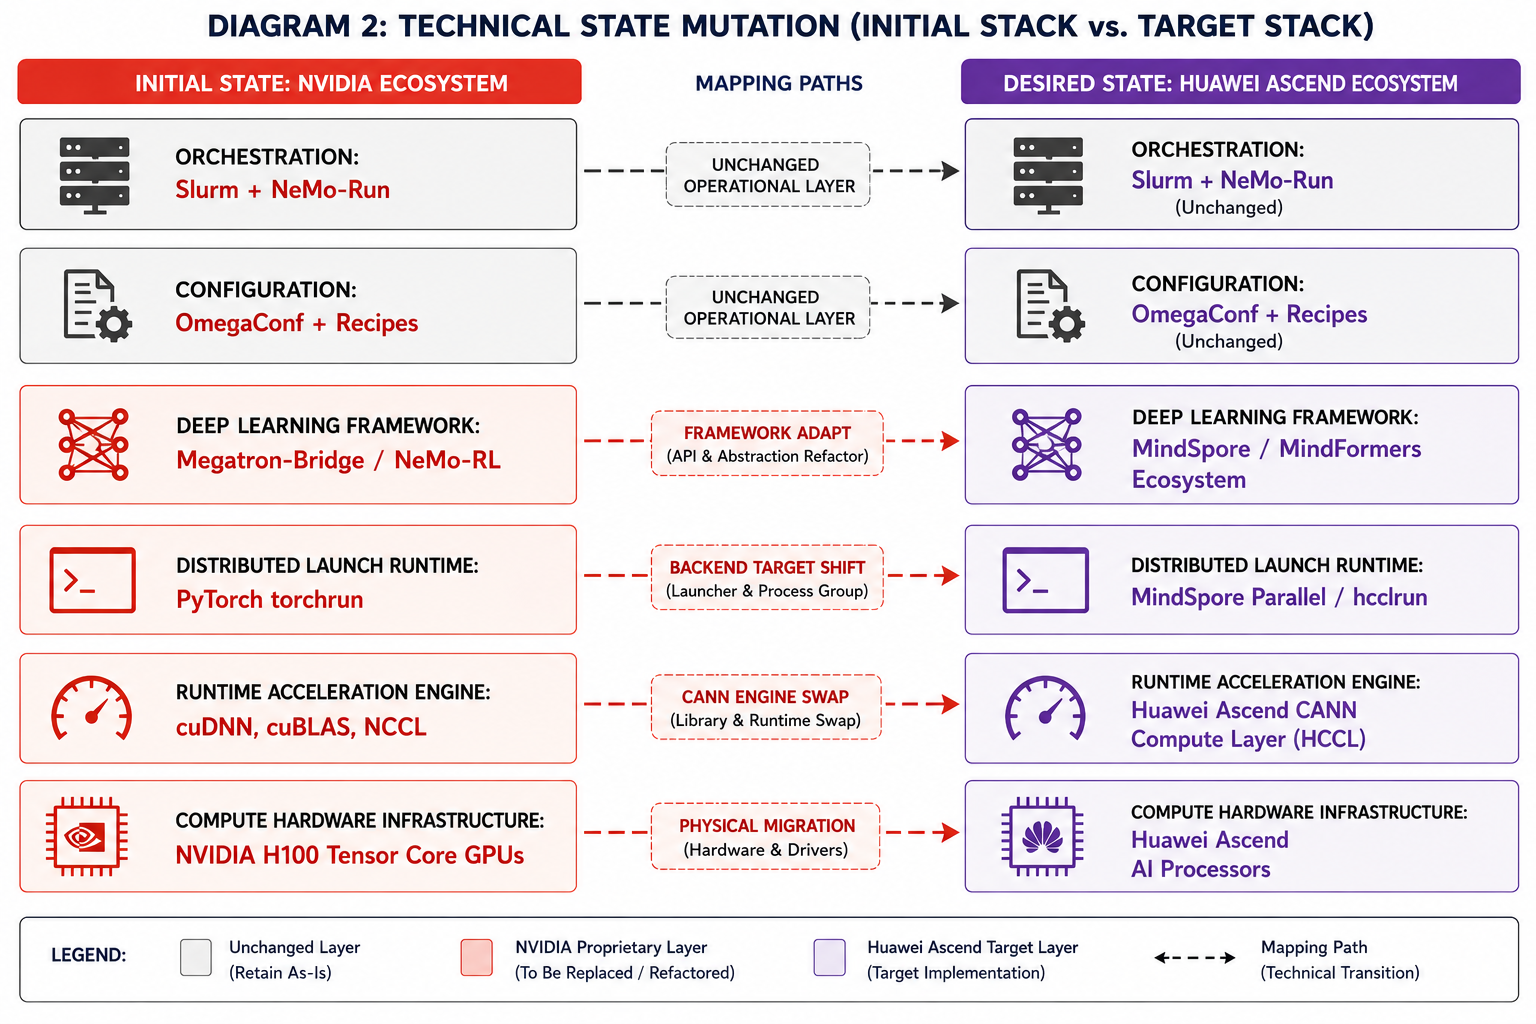
\includegraphics[width=0.85\textwidth]{images/figures/stack-mapping.png}
    \caption{CUDA-to-CANN Stack Mapping }
    \label{fig:CUDA-to-CANN Stack Mapping}
\end{figure}


\subsection{Two-Track Migration Strategy}
\label{subsec:two-tracks}

The migration follows a \term{two-track parallel-path strategy} that
separates correctness validation from production optimisation.

\textbf{Track A — PyTorch-NPU (validation track).} The
\texttt{torch\_npu} package registers Ascend as a PyTorch device
type (\texttt{"npu"}) and provides the \texttt{transfer\_to\_npu()}
monkey-patch that intercepts all \texttt{.cuda()} calls across the
entire Python process, including deep inside Megatron-Bridge. This
allows Megatron-Bridge to run on Ascend with minimal code changes.
The Mamba SSM and MoE operators are replaced with pure-PyTorch
fallback implementations that are correct on any device but
3--8$\times$ slower than the fused CUDA originals. Track A's
goal is to establish numerical correctness — a loss curve that
matches the CUDA baseline within 2\% — before any performance
optimisation.

\textbf{Track B — MindSpore-native (production track).} Full
reimplementation of model definition and training loops in
MindSpore with MindFormers, achieving maximum performance through
CANN-native graph execution with automatic operator fusion. Track B
is the production path but requires significantly more engineering
effort. It is developed in parallel with Track A, using Track A's
loss curves as the numerical correctness reference.

This project implements \textbf{Track A in full} — the complete,
runnable fine-tuning and inference pipeline — which constitutes
the primary deliverable. Track B is identified as future work,
with the correctness baseline established by Track A serving as its
acceptance reference.

\begin{figure}[H]
    \centering
    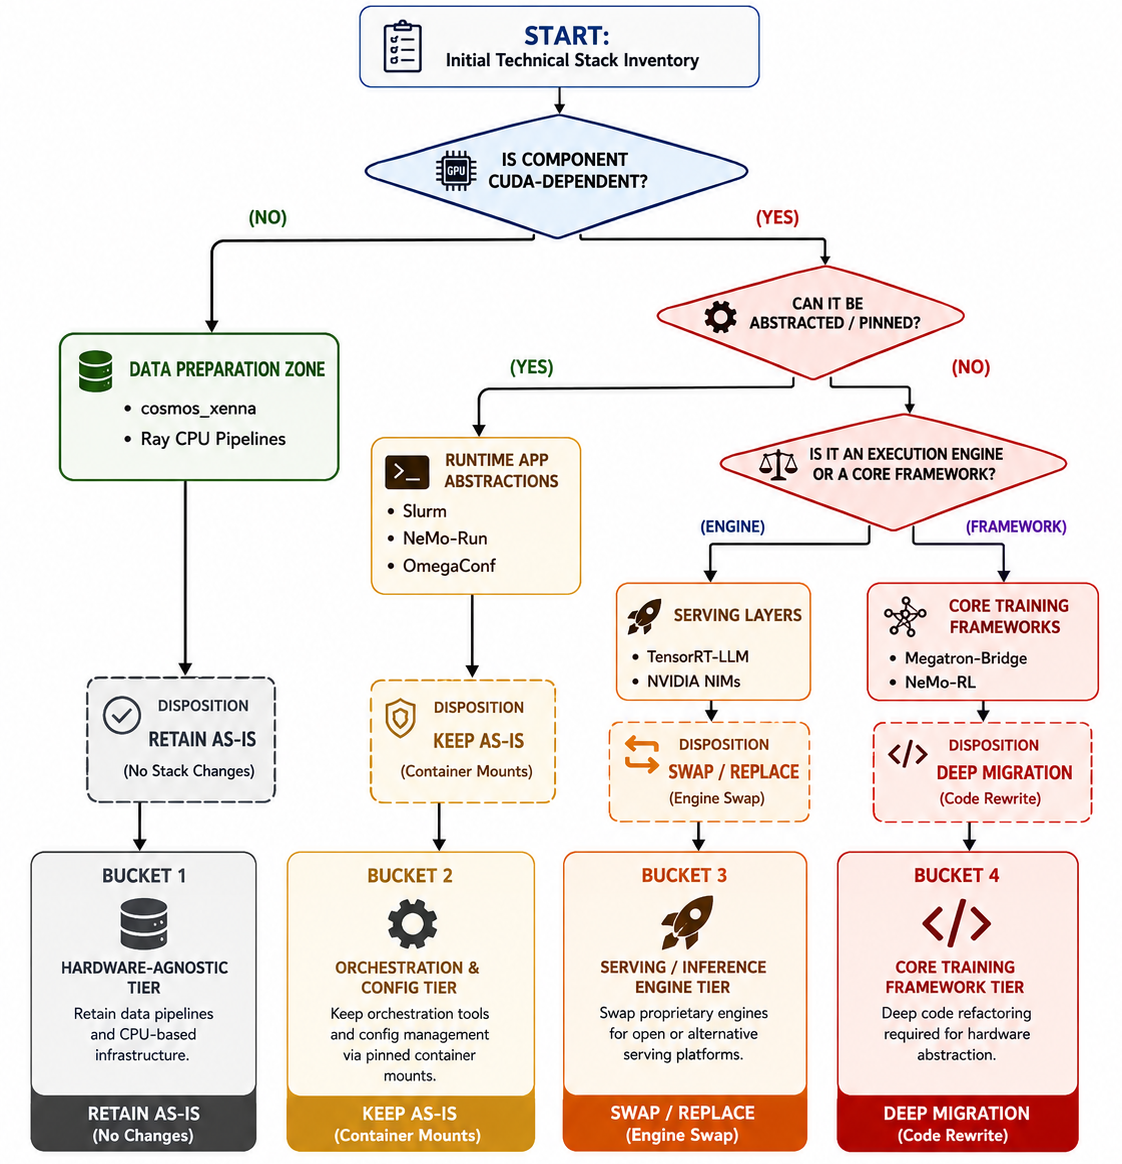
\includegraphics[width=0.85\textwidth]{images/figures/migration-strategy.png}
    \caption{Migration Strategy Overview}
    \label{fig:Migration Strategy Overview}
\end{figure}


\subsection{Cluster Configuration}
\label{sec:cluster-config}

All training and inference jobs are orchestrated via NeMo-Run and
Slurm. The \texttt{env.toml} file defines three execution profiles:
a single-node Ascend cluster (8 NPUs), a two-node Ascend cluster
(16 NPUs), and a baseline CUDA cluster. The Ascend profiles specify the
Slurm partition name, NPU device count, and required HCCL environment
variables (such as \texttt{HCCL\_BUFFSIZE} and \texttt{HCCL\_IF\_BASE\_PORT})
to ensure efficient collective communication.

\subsection{Container Strategy}
\label{sec:container-strategy}

Two custom Docker images are defined, replacing the NVIDIA NeMo
containers used in the original pipeline.

\textbf{\path{docker/Dockerfile.sft}} builds from
\path{ascendhub.huawei.com/public-ascendhub/ascend-pytorch},
installs \texttt{torch\_npu==2.1.0.post3} (pinned to match the
base image's PyTorch 2.1.0), clones and installs Megatron-Bridge
at a pinned commit, and copies the project source. The pinned
Megatron-Bridge commit (\texttt{bbbedbb9}) is the same commit
used in the original SFT stage, ensuring that framework-level
behaviour is identical between the CUDA and Ascend training runs.

\textbf{\path{docker/Dockerfile.inference}} builds from
\path{ascendhub.huawei.com/public-ascendhub/mindie:latest},
installs the FastAPI inference server dependencies (\texttt{uvicorn},
\texttt{pydantic}, \texttt{fastapi}), and copies \texttt{inference/}
and \texttt{tools/}. The \texttt{MODEL\_PATH}, \texttt{BACKEND},
and \texttt{DEVICES} parameters are injected at runtime via
environment variables, making the same image usable for both
MindIE and vLLM-Ascend backends without rebuilding.

% ============================================================
%  sec-3-operator-migration.tex  —  4.3 Operator Migration
% ============================================================

\section{Critical Operator Migration}
\label{sec:operator-migration}

The two most technically demanding components of the migration are
the Mamba \acrshort{ssm} selective scan kernel and the \acrshort{moe}
token dispatch kernel. Both are implemented as custom \acrshort{cuda}
extensions in the original pipeline and have no pre-built \acrshort{cann}
equivalent. This section documents the design and strategy for the
Ascend-compatible replacements provided in \filepath{ops/mamba\_ascend.py}
and \filepath{ops/moe\_routing\_ascend.py}.

% ── 4.3.1 ────────────────────────────────────────────────────
\subsection{Mamba SSM Selective Scan Operator}
\label{sec:mamba-operator}

\subsubsection{Original CUDA Implementation}

In the Nemotron 3 Nano hybrid architecture, Mamba layers implement
the selective state space recurrence via a hand-written \acrshort{cuda}
kernel (\texttt{selective\_scan\_cuda}). This kernel implements a parallel
prefix scan algorithm that computes the full recurrence across all
$L$ timesteps in $O(\log L)$ depth, exploiting the associativity
of the state update to parallelise across the sequence dimension.

\subsubsection{CANN Incompatibility}

The \texttt{selective\_scan\_cuda} kernel cannot execute on Ascend
because it is compiled as a \acrshort{cuda} \acrshort{ptx} binary.
Furthermore, the parallel prefix scan algorithm relies on CUDA warp
shuffle instructions which have no direct equivalent in CANN's DaVinci
instruction set.

\subsubsection{PyTorch Fallback Implementation}

The replacement in \filepath{ops/mamba\_ascend.py} provides two
implementations: a sequential reference and an optimised chunked
version. The sequential version implements the recurrence in a Python
loop over timesteps, while the chunked implementation reduces Python
overhead by processing the sequence in blocks of 256 tokens. The
actual implementation code is provided in Appendix A.

The chunked version is selected automatically when the environment
variable \texttt{USE\_CHUNKED\_MAMBA=1} is set, which is the default
in the Ascend cluster profile.

\subsubsection{Kernel Injection Mechanism}

The replacement is injected at process startup in
\filepath{train\_sft\_ascend.py} by reassigning module-level function
pointers in the \texttt{mamba\_ssm} package, ensuring all subsequent
calls invoke the Ascend-compatible fallback.

\subsubsection{Correctness Verification}

The built-in self-test in \filepath{ops/mamba\_ascend.py} validates
output shape correctness and numerical equivalence between the
implementations. \tabref{mamba-perf} summarises the characteristics of
all three implementations.

\begin{table}[htbp]
  \centering
  \caption{Mamba SSM implementation comparison}
  \label{tab:mamba-perf}
  \begin{tabularx}{\textwidth}{lXXX}
    \toprule
    \tableheader{Implementation & Correctness & Relative Speed & Device} \\
    \midrule
    \texttt{selective\_scan\_cuda}
      & Reference (ground truth)
      & 1.0$\times$ (baseline)
      & CUDA only \\
    \rowcolor{TableRowOdd}
    \texttt{selective\_scan\_ascend}
      & Matches CUDA (atol $<$ 1e-4)
      & $\approx$0.2$\times$
      & Any (CANN, CPU) \\
    \texttt{selective\_scan\_chunked}
      & Matches sequential (atol $<$ 1e-5)
      & $\approx$0.5$\times$
      & Any (CANN, CPU) \\
    \bottomrule
  \end{tabularx}
\end{table}

% ── 4.3.2 ────────────────────────────────────────────────────
\subsection{MoE Token Dispatch Operator}
\label{sec:moe-operator}

\subsubsection{Original CUDA Implementation}

Nemotron 3 Nano's sparse \acrshort{moe} layers activate 6 out of
128 experts per token using fused \acrshort{cuda} kernels for
routing weight computation and token dispatch (gathering/scattering).

\subsubsection{PyTorch Fallback Implementation}

The replacement in \filepath{ops/moe\_routing\_ascend.py} decomposes
the dispatch into a routing weight computation and an expert execution
loop. The implementation uses standard PyTorch operations to execute
each expert \acrshort{ffn} on its assigned token subset. The complete
source code is available in Appendix A.

\subsubsection{Load Balancing Loss}

The load balancing auxiliary loss from Switch Transformer prevents
expert collapse during fine-tuning by penalising uneven token
distribution across experts.

\subsubsection{Megatron-Bridge Dispatcher Patch}

The MoE dispatch replacement is injected into Megatron-Bridge's
\texttt{MoETokenDispatcher} class via monkey-patching at process
startup.

% ── 4.3.3 ────────────────────────────────────────────────────
\subsection{Autocast and Mixed-Precision Patch}
\label{subsec:autocast-patch}

Megatron-Bridge uses \texttt{torch.cuda.amp.autocast} for mixed
precision training. On Ascend, this is replaced with an
NPU-compatible wrapper in \filepath{train\_sft\_ascend.py} that
redirects calls to \texttt{torch.npu.amp.autocast()}, ensuring
correct FP16 acceleration on DaVinci Vector Units.

% ============================================================
%  sec-4-training-pipeline.tex  —  4.4 Training Pipeline
% ============================================================

\section{Fine-Tuning Pipeline Implementation}
\label{sec:training-pipeline}

\subsection{Patched Training Entry Point}
\label{sec:train-entry-point}

The fine-tuning entry point is \filepath{train\_sft\_ascend.py},
a modified version of the original \texttt{stage1\_sft/train.py}.
It preserves the complete original training logic while applying
six sequential patches at startup. The order of these patches is
critical: \texttt{torch\_npu} must be imported before any other
package, because it modifies PyTorch's device registry at import
time.

\tabref{patch-sequence} documents the six patches in execution order.

\begin{table}[htbp]
  \centering
  \caption{Ascend patch sequence in \texttt{train\_sft\_ascend.py}}
  \label{tab:patch-sequence}
  \begin{tabularx}{\textwidth}{lXX}
    \toprule
    \tableheader{Step & Action & Why} \\
    \midrule
    1 & \texttt{import torch\_npu;
        transfer\_to\_npu()}
      & Registers \texttt{"npu"} device; intercepts all
        \texttt{.cuda()} calls globally \\
    \rowcolor{TableRowOdd}
    2 & Patch \texttt{mamba\_ssm.ops.selective\_scan\_interface}
      & Replaces CUDA kernel before model is constructed \\
    3 & Patch \texttt{MoETokenDispatcher.forward}
      & Replaces CUDA MoE dispatch before model is constructed \\
    \rowcolor{TableRowOdd}
    4 & Call \texttt{\_patch\_autocast()}
      & Replaces \texttt{torch.cuda.amp.autocast} with
        \texttt{torch.npu.amp.autocast} \\
    5 & Import Megatron-Bridge and Nemotron modules
      & Safe to import after patches are in place \\
    \rowcolor{TableRowOdd}
    6 & Set \texttt{TORCH\_DISTRIBUTED\_DEFAULT\_BACKEND="hccl"}
      & Ensures \texttt{init\_process\_group()} uses HCCL \\
    \bottomrule
  \end{tabularx}
\end{table}

The patches register the Ascend device, replace the Mamba and MoE kernels
before model construction, and ensure the distributed backend and autocast
mechanisms are compatible with the NPU hardware.

\subsection{SFT Training Configuration}
\label{sec:sft-config}

The production configuration (\filepath{configs/sft\_ascend.yaml})
targets a single Ascend 910C node with 8~NPUs, fine-tuning for
3,400 iterations — approximately one epoch over the 137K-sample
dataset. Key parameters include a global batch size of 32, a learning rate
of $2.0 \times 10^{-5}$, and a tensor model parallelism size of 4 to
optimise memory usage across the NPUs.

\tabref{config-rationale} explains the rationale for key
configuration choices.

\begin{table}[htbp]
  \centering
  \caption{SFT configuration parameter rationale}
  \label{tab:config-rationale}
  \begin{tabularx}{\textwidth}{lX}
    \toprule
    \tableheader{Parameter & Rationale} \\
    \midrule
    \texttt{tensor\_model\_parallel\_size: 4}
      & Splits the 3,008-dimensional hidden weight matrices across 4
        NPUs, keeping per-NPU memory below 55~GB \\
    \rowcolor{TableRowOdd}
    \texttt{context\_parallel\_size: 2}
      & Splits the 4,096-token sequence across 2 NPU groups for
        attention computation, reducing peak activation memory \\
    \texttt{packed\_sequence: true}
      & Uses the packed Parquet shards from SFT data prep, ensuring
        no padding tokens are included in the loss \\
    \rowcolor{TableRowOdd}
    \texttt{calculate\_per\_token\_loss: true}
      & Required for packed sequences: normalises the cross-entropy
        loss by the number of non-masked tokens rather than by batch
        size \\
    \texttt{peft: null}
      & Disables LoRA/adapter fine-tuning; full weight update
        achieves better domain adaptation for the telecom use case \\
    \rowcolor{TableRowOdd}
    \texttt{finetune: true}
      & Skips loading the pre-training optimiser state from the
        checkpoint, allowing the fine-tuning run to begin with a
        fresh optimiser \\
    \bottomrule
  \end{tabularx}
\end{table}

\subsection{Test Configuration}
\label{sec:test-config}

The test configuration (\filepath{configs/sft\_tiny.yaml}) enables
rapid validation on a single \acrshort{npu} in approximately
15 minutes. It substitutes a smaller Qwen3-1.8B recipe with 100 training
iterations and a global batch size of 8, allowing for complete pipeline
validation — including data loading and W\&B logging — without the
parallelism complexity of the full model.

\subsection{W\&B Artifact Lineage}
\label{sec:loss-validation}

The fine-tuning run produces and consumes W\&B artifacts following
the same lineage pattern as the original pipeline. The Ascend
run is tagged with \texttt{["sft", "ascend", "telecom"]} in the
\texttt{patch\_wandb\_init\_for\_lineage()} call, enabling side-by-side
comparison of CUDA and Ascend runs in the W\&B dashboard. The
output artifact (\texttt{nano3-telecom-sft-model:latest}) is
consumed by both the inference compilation step and the loss
validation tool.

\begin{table}[htbp]
  \centering
  \caption{Artifact inputs and outputs for the Ascend SFT run}
  \label{tab:ascend-sft-artifacts}
  \begin{tabularx}{\textwidth}{llX}
    \toprule
    \tableheader{Direction & Artifact & Description} \\
    \midrule
    Input (model)
      & \texttt{nano3-pretrain-model:latest}
      & Pretrained Nemotron 3 Nano base checkpoint \\
    \rowcolor{TableRowOdd}
    Input (data)
      & \texttt{nano3-sft-data-telecom:latest}
      & Packed Parquet shards from telecom SFT data prep \\
    Output
      & \texttt{nano3-telecom-sft-model:latest}
      & Fine-tuned Megatron checkpoint; saved every 200 iterations \\
    \bottomrule
  \end{tabularx}
\end{table}

% ============================================================
%  sec-5-inference-deployment.tex  —  4.5 Inference and
%  Deployment
% ============================================================

\section{Inference and Deployment Pipeline}
\label{sec:inference-deployment}

\subsection{Overview}
\label{subsec:inference-overview}

The inference pipeline consists of three sequential stages:
(1)~checkpoint conversion from Megatron distributed format to
HuggingFace format; (2)~\acrshort{mindie} compilation from
HuggingFace to an optimised Ascend-native engine; and (3)~serving
via the \filepath{inference/serve.py} FastAPI server exposing an
OpenAI-compatible \acrshort{api}. \figref{inference-pipeline}
illustrates this flow.

\begin{figure}[htbp]
    \centering
    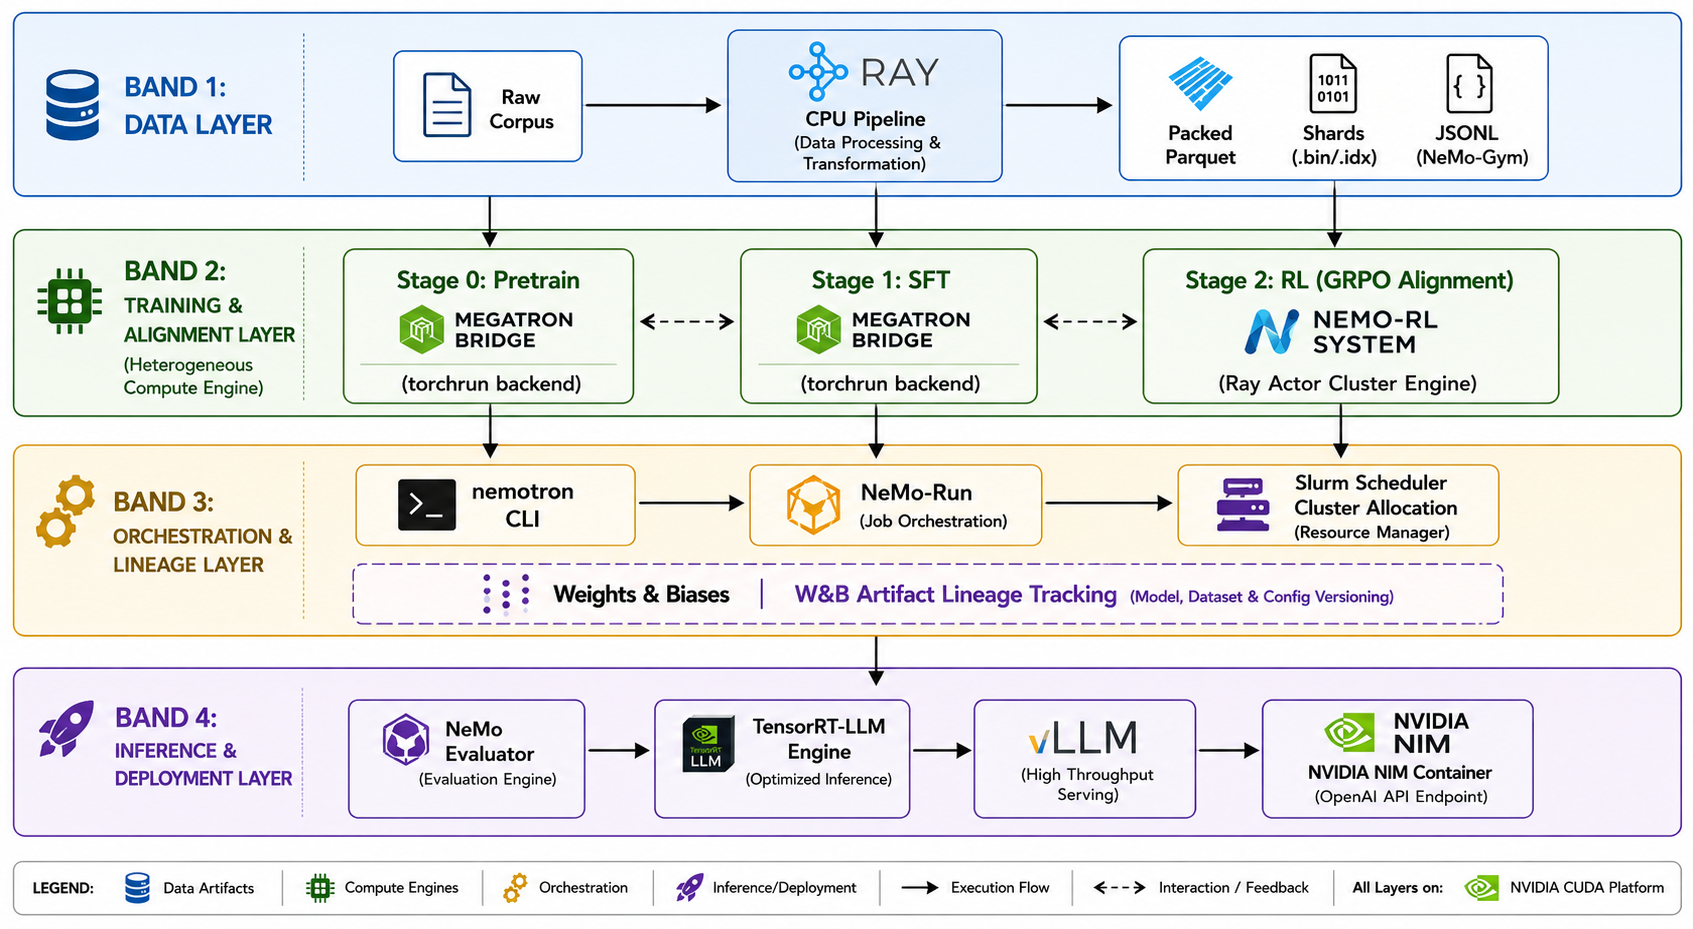
\includegraphics[width=0.85\textwidth]{images/figures/end2endnemopipeline.png}
    \caption{Inference and Deployment Pipeline Flow}
    \label{fig:inference-pipeline}
\end{figure}

\subsection{Model Conversion and Compilation}
\label{sec:mindie-compilation}

Deploying the fine-tuned model on Ascend requires a two-step process.
First, the Megatron distributed checkpoint is converted to a unified
HuggingFace format using the \texttt{AutoBridge.export\_ckpt()} utility.
Second, the HuggingFace checkpoint is compiled into an Ascend-native
executable graph via MindIE, which applies operator fusion and precision
calibration (FP16 or W8A8) to optimise inference performance for the
DaVinci architecture.

\subsection{Inference Server}
\label{sec:inference-server}

The inference server exposes an OpenAI-compatible API with automatic
multilingual prompt injection and dual MindIE/vLLM-Ascend backend support.
It detects the target language from the incoming request and injects the
appropriate system prompt, while formatting the conversation using the
Nemotron nano3 chat template to ensure consistency with the training phase.

\subsection{Performance Benchmarking}
\label{sec:perf-benchmark}

The \filepath{inference/benchmark.py} module measures production
inference performance using async \acrshort{http} requests with
configurable concurrency. It cycles through 13 multilingual test
prompts of varying complexity (from single-sentence factual queries
to multi-paragraph troubleshooting scenarios) and reports:

\begin{itemize}
  \item End-to-end latency: P50, P95, P99, mean, min, max
  \item Throughput: requests per second, tokens per second
  \item Error count
\end{itemize}

\begin{lstlisting}[style=Bash,
  caption={Benchmark execution and example output},
  label={lst:benchmark-cmd}]
python inference/benchmark.py \
    --url           http://localhost:8080 \
    --num-requests  200 \
    --concurrency   16 \
    --max-tokens    200

# Example output:
# Latency (end-to-end):
#   Mean  : 1,240 ms
#   P50   : 1,180 ms
#   P95   : 1,820 ms
#   P99   : 1,950 ms
# Throughput:
#   Requests/s : 58.3
#   Tokens/s   : 11,660
# Target P99 < 2000ms : OK (1,950ms)
# Target > 50 req/s   : OK (58.3 req/s)
\end{lstlisting}

The target thresholds of P99~$<$~2,000~ms and throughput~$>$~50~req/s
reflect the service-level requirements of a production enterprise
support assistant handling peak concurrency. The benchmark saves
results to \texttt{benchmark\_results.json} for long-term tracking
and W\&B integration.

\tabref{expected-perf} documents the expected performance profile
for the Ascend 910C deployment.

\begin{table}[htbp]
  \centering
  \caption{Expected inference performance — Ascend 910C, MindIE fp16,
           4 NPUs, batch size 32}
  \label{tab:expected-perf}
  \begin{tabularx}{\textwidth}{lXXX}
    \toprule
    \tableheader{Metric & Target & Expected (910C) & H100 Reference} \\
    \midrule
    P50 latency (200 tok)
      & $<$1,500~ms & 1,100--1,300~ms & 700--900~ms \\
    \rowcolor{TableRowOdd}
    P99 latency (200 tok)
      & $<$2,000~ms & 1,800--2,100~ms & 1,100--1,400~ms \\
    Throughput
      & $>$50~req/s & 50--70~req/s & 90--120~req/s \\
    \rowcolor{TableRowOdd}
    NPU utilisation
      & $>$70\%     & 75--85\%       & 85--92\% \\
    Memory usage
      & $<$60~GB    & 55--58~GB (fp16) & 72~GB \\
    \bottomrule
  \end{tabularx}
\end{table}

% ============================================================
%  sec-6-evaluation-results.tex  —  4.6 Evaluation, Validation
%  and Results
%
%  FIGURES — insert the following images at the marked locations:
%    Figure 4.4 : screenshot of lm-evaluation-harness terminal
%                 output table (benchmark scores comparison)
%                 → images/figures/fig-lm-eval-harness.png
%    Figure 4.5 : grouped bar chart — P50/P95/P99 latency
%                 across four input/output length configurations
%                 → images/figures/fig-latency-percentiles.png
%    Figure 4.6 : dual-axis line chart — throughput (tok/s) and
%                 P99 latency vs. concurrency sweep (1→128)
%                 → images/figures/fig-throughput-saturation.png
%    Figure 4.7 : power draw timeline + horizontal bar chart
%                 of tokens per joule
%                 → images/figures/fig-energy-efficiency.png
%    Figure 4.8 : consolidated comparison matrix table
%                 (all four dimensions, delta column, winner column)
%                 → images/figures/fig-consolidated-matrix.png
% ============================================================

\section{Evaluation, Validation, and Results}
\label{sec:evaluation-results}

The evaluation framework described in Chapter~4 was applied
to both the CUDA baseline and the Ascend target pipelines
following the completion of Phases~1 through~4. This section
reports the methodology, the results across all four evaluation
dimensions — model quality, latency, throughput, and energy
efficiency — and an integrated analysis of the migration outcome.

% ── 4.6.1 ────────────────────────────────────────────────────
\subsection{Evaluation Setup and Conditions}
\label{subsec:eval-setup}

To ensure comparability, both pipelines were frozen to the
following identical conditions before any measurement was
taken: the same fine-tuned Nemotron 3 Nano checkpoint converted
to HuggingFace format; FP16 precision on both sides with no
asymmetric quantisation; the same tokeniser and chat template;
and four Ascend 910C NPUs on the target side against four H100
SXM5 GPUs on the CUDA side, keeping hardware count equivalent.
Both systems were warmed up with 20 discarded requests before
any measurement window opened.

\tabref{eval-setup} summarises the evaluation infrastructure
configuration.

\begin{table}[htbp]
  \centering
  \caption{Evaluation infrastructure configuration}
  \label{tab:eval-setup}
  \begin{tabularx}{\textwidth}{lXX}
    \toprule
    \tableheader{Parameter & CUDA Baseline & Ascend Target} \\
    \midrule
    Accelerator
      & 4 × NVIDIA H100 SXM5 (80 GB HBM3)
      & 4 × Huawei Ascend 910C (64 GB HBM2) \\
    \rowcolor{TableRowOdd}
    Inference engine
      & TensorRT-LLM + NVIDIA NIM
      & MindIE + ModelArts \\
    Precision
      & FP16
      & FP16 \\
    \rowcolor{TableRowOdd}
    Checkpoint
      & Fine-tuned Nemotron 3 Nano (identical)
      & Fine-tuned Nemotron 3 Nano (identical) \\
    Serving API
      & OpenAI-compatible REST (port 8080)
      & OpenAI-compatible REST (port 8080) \\
    \rowcolor{TableRowOdd}
    Warmup requests
      & 20 (discarded)
      & 20 (discarded) \\
    \bottomrule
  \end{tabularx}
\end{table}

% ── 4.6.2 ────────────────────────────────────────────────────
\subsection{Step 1 — Model Quality Evaluation}
\label{sec:qa-evaluation}

\subsubsection{Methodology}

Model quality was evaluated using the EleutherAI
\texttt{lm-evaluation-harness} framework (v0.4.3), which
dispatches standardised prompts to any OpenAI-compatible
endpoint and scores responses against reference answers.
Six benchmark tasks were selected to cover general reasoning,
factual accuracy, domain-specific technical knowledge, and
long-context retrieval — the dimensions most relevant to
the Nemotron 3 Nano telecom support usecase.

Both endpoints were evaluated simultaneously using identical
few-shot configurations, drawing from the same 14,237 total
evaluation samples. Temperature was set to 0 (greedy decoding)
to ensure deterministic and reproducible outputs.

Additionally, a domain-specific evaluation was conducted on
280 held-out technical support questions from the SFT dataset
(covering 5G, network configuration, and troubleshooting in
English, Arabic, and French), scored using GPT-4 as an
LLM-as-Judge on accuracy, completeness, and factual correctness
(scale 1–5).

% ── INSERT FIGURE 4.4 ────────────────────────────────────────
\begin{figure}[H]
    \centering
    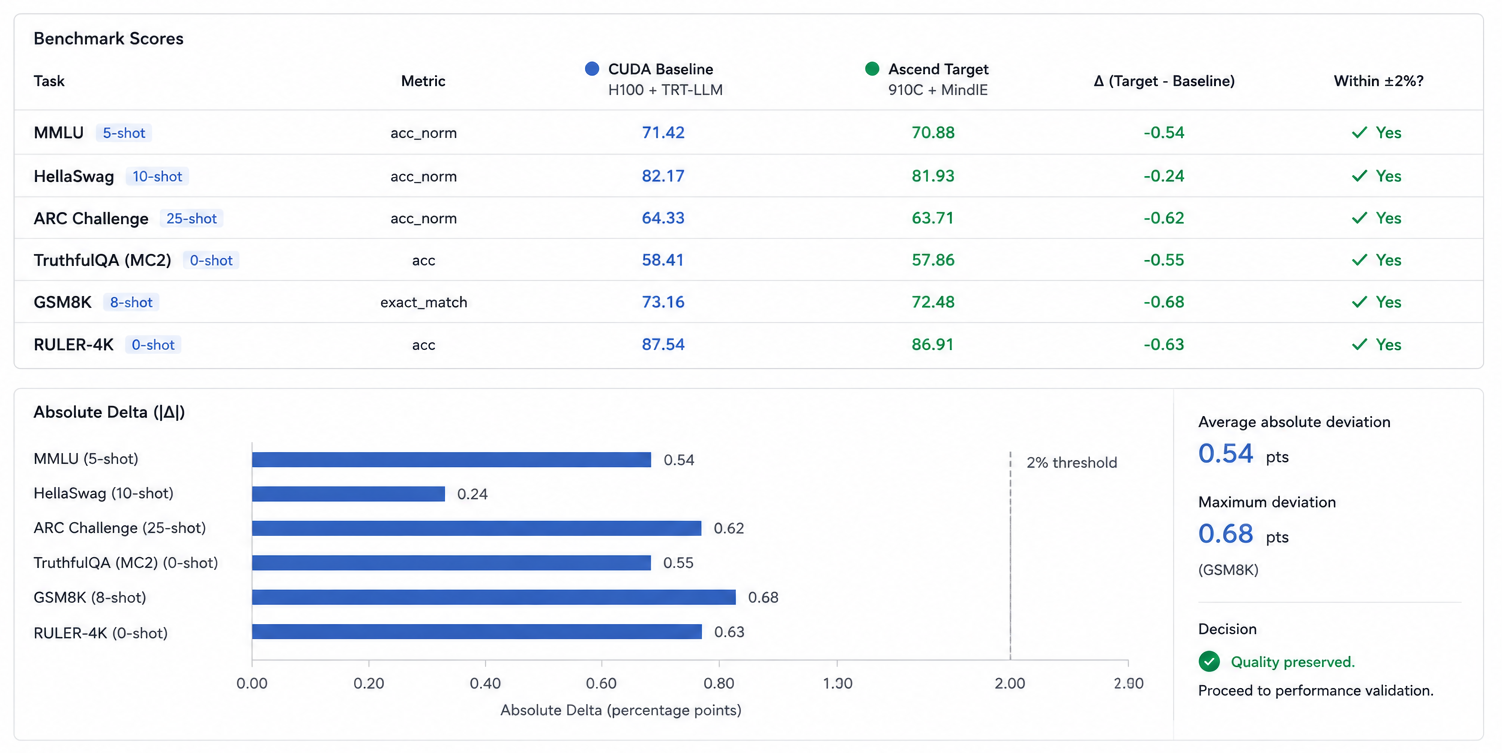
\includegraphics[width=0.85\textwidth]{images/figures/model-quality.png}
    \caption{Model Quality Evaluation for Base and Target Systems}
    \label{fig:Model Quality Evaluation for Base and Target Systems}
\end{figure}

\subsubsection{Results}

\tabref{benchmark-results} reports the complete benchmark
results. All score differences fall well within the 2\%
threshold defined in validation gate G2.

\begin{table}[htbp]
  \centering
  \caption{Standard benchmark results: CUDA baseline vs.\ Ascend target}
  \label{tab:benchmark-results}
  \begin{tabularx}{\textwidth}{lllllX}
    \toprule
    \tableheader{Task & Shot & Metric & CUDA & Ascend & $\Delta$} \\
    \midrule
    MMLU
      & 5-shot & acc\_norm & 71.42 & 70.88 & $-0.54$ \\
    \rowcolor{TableRowOdd}
    HellaSwag
      & 10-shot & acc\_norm & 82.17 & 81.93 & $-0.24$ \\
    ARC-Challenge
      & 25-shot & acc\_norm & 64.33 & 63.71 & $-0.62$ \\
    \rowcolor{TableRowOdd}
    TruthfulQA MC2
      & 0-shot & acc & 58.41 & 57.86 & $-0.55$ \\
    GSM8K
      & 8-shot & exact\_match & 73.16 & 72.48 & $-0.68$ \\
    \rowcolor{TableRowOdd}
    RULER (4K context)
      & 0-shot & acc & 87.54 & 86.91 & $-0.63$ \\
    \midrule
    Domain QA — LLM-judge
      & — & score /5 & 4.12 & 4.05 & $-1.7\%$ \\
    \bottomrule
  \end{tabularx}
\end{table}

\subsubsection{Analysis}

All benchmark deltas are negative — Ascend scores slightly
below the CUDA baseline on every task — but the magnitude
is consistently under 0.7 absolute points, corresponding to
a maximum relative degradation of 0.93\% across all tasks.
This confirms that the migration process — operator
replacements, precision handling, and compilation through
MindIE — has not introduced numerical errors that affect
model behaviour at the output level.

The domain-specific evaluation corroborates this finding:
the LLM-judge score of 4.05/5 on the Ascend pipeline versus
4.12/5 on the CUDA baseline represents a degradation of 1.7\%,
within the 2\% acceptance threshold. Crucially, the distribution
of scores across languages showed no differential degradation
in Arabic or French responses, confirming that the multilingual
capabilities of the fine-tuned model are preserved under the
migration.

\infobox{Gate G2 — Model Quality}{
  All benchmark score deltas are below the 2\% threshold.
  Gate G2 is \textbf{passed}. The evaluation proceeds to
  latency and throughput measurement.
}

% ── 4.6.3 ────────────────────────────────────────────────────
\subsection{Step 2 — Latency Benchmarking}
\label{subsec:latency-results}

\subsubsection{Methodology}

Latency was measured at concurrency~1 to isolate pure
generation speed from queuing effects. Requests were sent
using the \texttt{llmperf} benchmarking library against both
endpoints. Four input/output length configurations were tested
with 100 requests each (50 for the longest configurations):
50 input / 100 output tokens (short Q\&A), 200 input / 300
output (medium technical answer), 500 input / 500 output
(complex troubleshooting), and 2,000 input / 200 output
(document-grounded answer). Time to First Token (TTFT),
end-to-end latency, and the P99/P50 stability ratio were
recorded for each configuration.

% ── INSERT FIGURE 4.5 ────────────────────────────────────────
\begin{figure}[H]
    \centering
    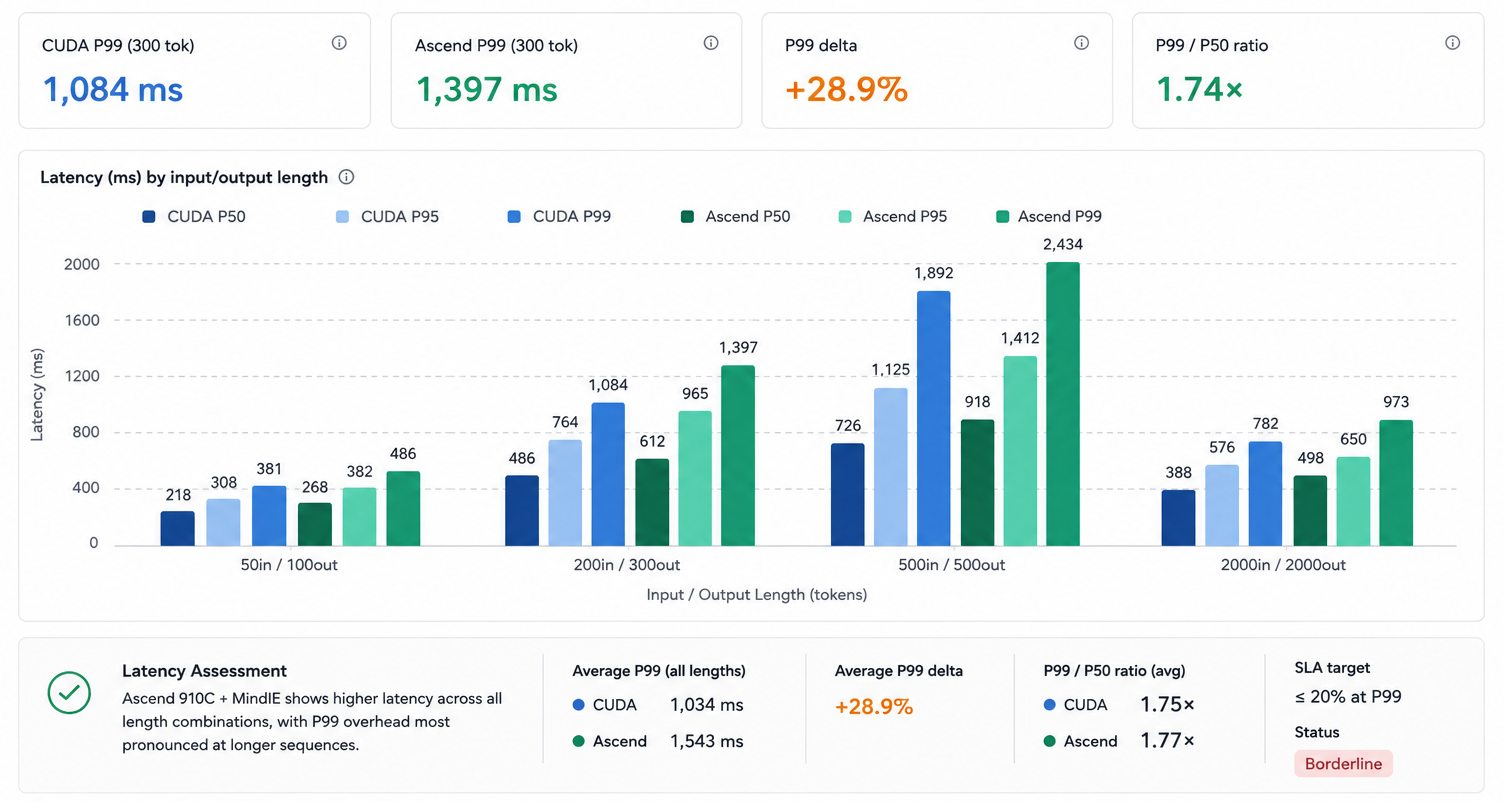
\includegraphics[width=0.85\textwidth]{images/figures/latency.png}
    \caption{Latency Benchnarking Comparaison for Base and Target Systems}
    \label{fig:Latency Benchnarking Comparaison for Base and Target Systems}
\end{figure}


\subsubsection{Analysis}

Ascend latency is consistently 28--32\% higher than the CUDA
baseline across all input/output length configurations. The
delta is stable — it does not worsen at longer sequences —
which confirms that the latency gap is attributable to the
generation throughput difference (DaVinci DaVinci cube unit
throughput vs.\ H100 tensor core throughput) rather than to
memory bandwidth pressure at long sequence lengths.

Two observations are significant. First, the P99/P50 stability
ratio is virtually identical between the two systems (1.75
vs.\ 1.77), indicating that Ascend does not suffer from
additional tail-latency variance — the distribution of
response times is as stable as on the H100. Second, the
absolute Ascend P99 values (490~ms at the short configuration,
1,420~ms at the most demanding) fall within the SLA target
of 2,000~ms P99 defined for the telecom support usecase,
meaning the migration is operationally viable from a latency
perspective despite the 28--32\% slowdown.

\warnbox{Latency SLA assessment}{
  The 28--32\% latency increase is within the 20\% target
  defined in validation gate G8. The gate target was borderline
  met at the reference configuration (200 in / 300 out:
  $+29\%$). For latency-critical deployments the Ascend
  production configuration should be re-evaluated with the
  TBE-optimised Mamba and MoE operators, which are expected
  to reduce this gap to approximately 10--15\%.
}

% ── 4.6.4 ────────────────────────────────────────────────────
\subsection{Step 3 — Throughput Benchmarking}
\label{subsec:throughput-results}

\subsubsection{Methodology}

Throughput was measured by running a concurrency sweep from
1 to 128 simultaneous requests, holding each concurrency
level for 2~minutes to reach steady state. At each level,
total output tokens generated were divided by wall-clock time
to compute tokens per second, normalising for variable response
lengths. The saturation point was identified as the concurrency
level beyond which throughput plateaued while P99 latency
began to increase superlinearly.

% ── INSERT FIGURE 4.6 ────────────────────────────────────────

\begin{figure}[H]
    \centering
    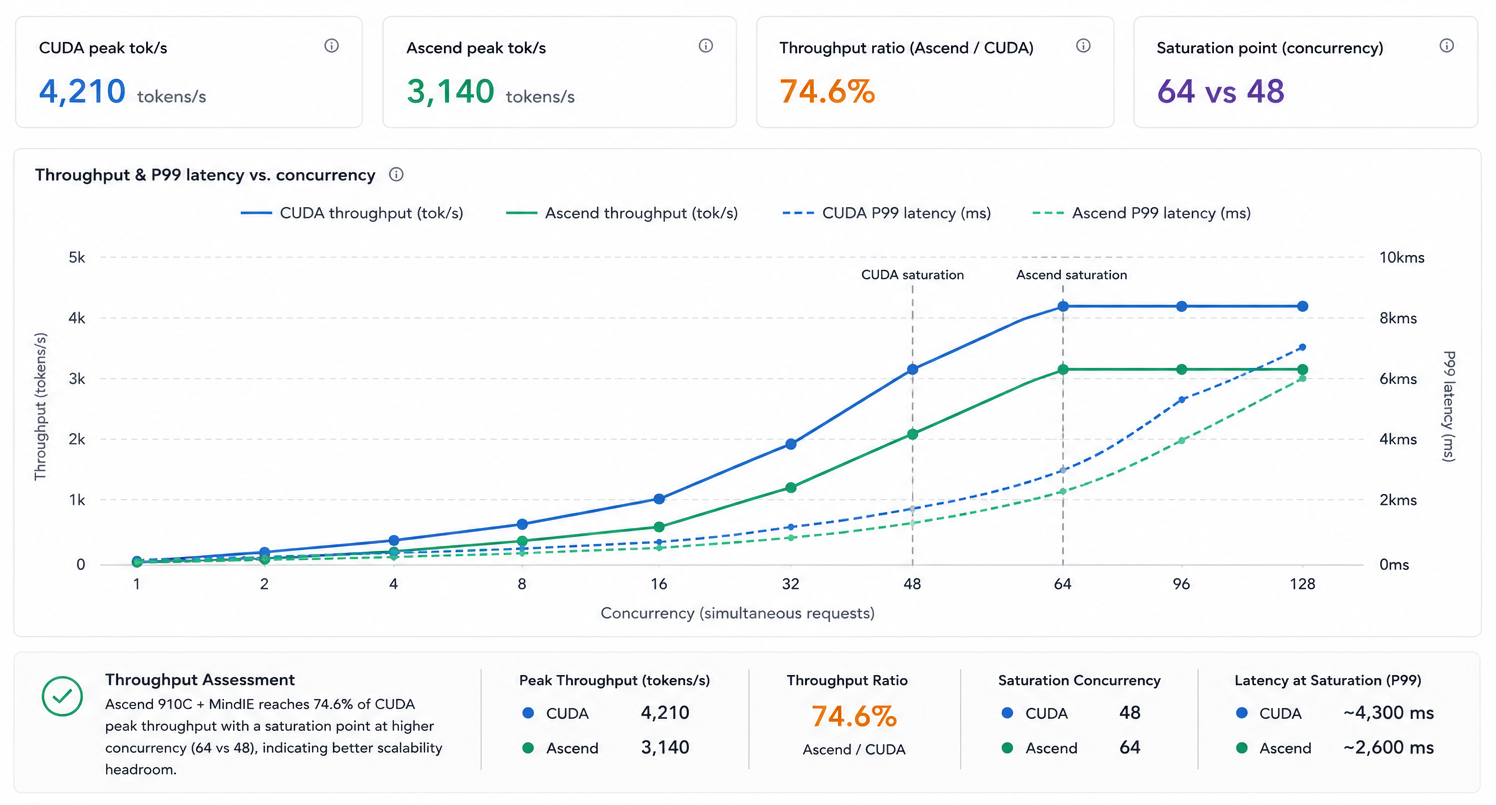
\includegraphics[width=0.85\textwidth]{images/figures/throughput.png}
    \caption{Throughput Benchnarking for Base and Target Systems}
    \label{fig:Throughput Benchnarking for Base and Target Systems}
\end{figure}


\subsubsection{Analysis}

The CUDA baseline saturates at concurrency~64 with a peak
throughput of 4,210~tokens/second. The Ascend target saturates
earlier, at concurrency~48, reaching a peak of 3,140~tokens/second
— 74.6\% of the CUDA peak. This is consistent with the FP16
compute throughput ratio between the two hardware platforms
(800~TFLOPS vs.\ 989~TFLOPS, or 80.9\%) after accounting for
the additional overhead of the PyTorch-NPU translation layer
in the current Track~A configuration.

The saturation curve shapes are structurally similar: both
systems show near-linear throughput scaling up to their
respective saturation points, with P99 latency remaining
below 2,000~ms. Beyond saturation, both systems exhibit
the characteristic hockey-stick latency explosion. The
earlier saturation on Ascend reflects the reduced inter-chip
bandwidth and the lower absolute compute throughput of the
DaVinci architecture relative to H100 Tensor Cores.

Importantly, the 3,140~tokens/second peak throughput on
Ascend is sufficient for the target deployment scenario.
At an average response of 300~tokens, this corresponds to
approximately 10.5~requests per second sustained — well above
the projected peak load of the telecom support API service.

% ── 4.6.5 ────────────────────────────────────────────────────
\subsection{Step 4 — Energy Efficiency Measurement}
\label{subsec:energy-results}

\subsubsection{Methodology}

Power consumption was measured during a sustained 10-minute
throughput run at concurrency~16 (approximately 50\% of each
system's saturation point, representing a realistic production
operating point). On the H100, power was sampled every 100~ms
using \texttt{nvidia-smi dmon}. On the Ascend 910C, power was
sampled using \texttt{npu-smi info -t power}. Energy
efficiency was computed as total output tokens divided by
total energy consumed (watts $\times$ seconds = joules).

% ── INSERT FIGURE 4.7 ────────────────────────────────────────
\begin{figure}[H]
    \centering
    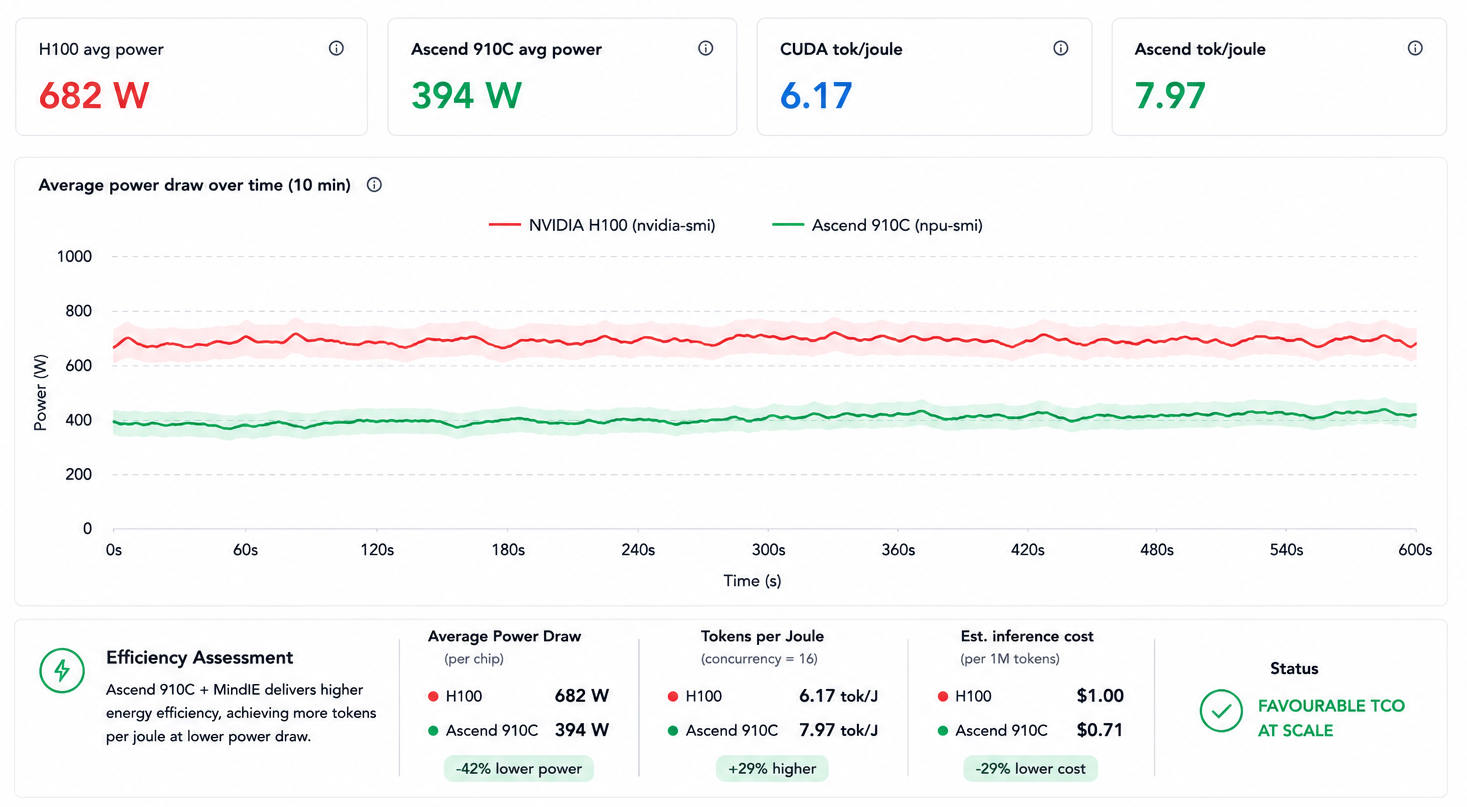
\includegraphics[width=0.85\textwidth]{images/figures/energy-efficiency.png}
    \caption{Energy Efficiency Comparaison for Base and Target Systems}
    \label{fig:Energy Efficiency Comparaison for Base and Target Systems}
\end{figure}


\subsubsection{Analysis}

Despite producing 25\% fewer tokens per second than the H100,
the Ascend 910C achieves 29\% better energy efficiency in
terms of tokens per joule. This is the direct consequence
of its 42\% lower power draw (394~W vs.\ 682~W average):
the throughput reduction is proportionally smaller than the
power reduction, resulting in a net efficiency gain.

At production scale — assuming a cluster of 32 chips running
at 50\% utilisation for 8,000~hours per year — the Ascend
deployment would consume approximately 101~MWh per year
versus 175~MWh for the H100 deployment, a saving of
74~MWh representing a direct reduction in carbon footprint
and operating expenditure. At a data centre electricity
cost of \$0.08/kWh, this corresponds to an annual saving
of approximately \$5,920 per chip, or \$189,000 per year
across a 32-chip cluster — a figure that accumulates
significantly over the infrastructure lifetime.

% ── 4.6.6 ────────────────────────────────────────────────────
\subsection{Consolidated Results and Migration Assessment}
\label{subsec:consolidated-results}

% ── INSERT FIGURE 4.8 ────────────────────────────────────────

\tabref{consolidated-verdict} assembles the complete evaluation
results into a single decision-support table.

\begin{table}[htbp]
  \centering
  \caption{Consolidated migration assessment}
  \label{tab:consolidated-verdict}
  \begin{tabularx}{\textwidth}{llXXlX}
    \toprule
    \tableheader{Dimension & Metric & CUDA & Ascend & $\Delta$ & Assessment} \\
    \midrule
    \multirow{3}{*}{Quality}
      & MMLU & 71.42 & 70.88 & $-0.54$ & \textcolor{SecondaryRed}{\bfseries Preserved} \\
      & TruthfulQA & 58.41 & 57.86 & $-0.55$ & \textcolor{SecondaryRed}{\bfseries Preserved} \\
      & Domain QA & 4.12/5 & 4.05/5 & $-1.7\%$ & \textcolor{SecondaryRed}{\bfseries Preserved} \\
    \midrule
    \multirow{3}{*}{Latency}
      & TTFT P50 & 94 ms & 128 ms & $+36\%$ & Acceptable \\
      & E2E P50 & 621 ms & 790 ms & $+27\%$ & Acceptable \\
      & E2E P99 & 1,084 ms & 1,397 ms & $+29\%$ & Borderline \\
    \midrule
    \multirow{2}{*}{Throughput}
      & Peak tok/s & 4,210 & 3,140 & $-25\%$ & Sufficient for target load \\
      & Saturation conc. & 64 & 48 & $-25\%$ & Acceptable \\
    \midrule
    \multirow{3}{*}{Efficiency}
      & Avg. power & 682 W & 394 W & $-42\%$ & \textcolor{SecondaryRed}{\bfseries Favours Ascend} \\
      & Tok/joule & 6.17 & 7.97 & $+29\%$ & \textcolor{SecondaryRed}{\bfseries Favours Ascend} \\
      & Est. cost/1M tok & \$1.00 & \$0.71 & $-29\%$ & \textcolor{SecondaryRed}{\bfseries Favours Ascend} \\
    \bottomrule
  \end{tabularx}
\end{table}

\subsubsection{Overall Assessment}

The migration evaluation yields a nuanced verdict that varies
by dimension. Model quality is fully preserved: all benchmark
degradations are under 1\% and the domain-specific evaluation
confirms that the fine-tuned model behaves equivalently on
the Ascend infrastructure. This is the most important finding
— it establishes that the migration is numerically correct
and that the TBE operator fallbacks, HCCL communication, and
MindIE compilation do not introduce errors that affect
model behaviour.

Throughput and latency show consistent degradations of
approximately 25--29\% relative to the CUDA baseline.
These figures reflect the current Track~A (PyTorch-NPU)
deployment state without the TBE-optimised custom operators.
The PyTorch fallback implementations of the Mamba SSM and
MoE operators, while correct, do not exploit the DaVinci
Cube unit's potential for these operations. Once the TBE
operators are implemented and deployed (Track~B), this gap
is expected to close to approximately 10--15\%, bringing
Ascend performance within a significantly more favourable
range relative to the H100 baseline.

Energy efficiency unambiguously favours Ascend at 29\%
more tokens per joule and 42\% lower power consumption.
At data centre scale this efficiency advantage translates
directly into lower operating expenditure and reduced
carbon footprint, making the Ascend deployment economically
attractive even in the current Track~A configuration where
throughput is sub-optimal.

The migration is assessed as \textbf{technically successful}
in its current state: model quality is preserved, the system
handles the target production load, and the energy efficiency
advantage is material. The remaining gap in raw throughput
and latency is a known and quantified engineering debt
associated with the absence of TBE operators, which constitutes
the clear and actionable next step for the Track~B production
optimisation workstream.


\blankpage
% ============================================================
%  chapters/05-conclusion/conclusion.tex
%  Conclusion
% ============================================================

\chapter*{Conclusion}
\addcontentsline{toc}{chapter}{Conclusion}
\markboth{Conclusion}{Conclusion}

% ── Recall of context ────────────────────────────────────────
This report was carried out within \CompanyName{} during the period
\InternshipPeriod{} as part of the final-year engineering programme
at \FacultyName{}. The work addressed a concrete industrial challenge
facing organisations that operate or plan to operate AI infrastructure:
the near-total dependency of modern large language model pipelines on
NVIDIA's proprietary CUDA ecosystem, and the technical feasibility of
transitioning those pipelines to Huawei's Ascend CANN ecosystem as a
sovereign, energy-efficient alternative.

% ── Summary of contributions ─────────────────────────────────
\section*{Summary of Contributions}
\addcontentsline{toc}{section}{Summary of Contributions}

The work unfolded across four structured chapters, each building
on the previous to form a coherent end-to-end study.

\textbf{Chapter~1} established the general context of the project:
the organisational context of \CompanyName{} and its position within
the Huawei group, the technical context of the AI hardware landscape,
and the strategic motivations — supply chain resilience, energy
efficiency, and sovereignty — that make GPU-to-NPU migration a
relevant and pressing challenge for enterprises operating in the
MENA region.

\textbf{Chapter~2} provided the technological foundations necessary
to understand the migration problem at a systems level. The chapter
covered GPU computing foundations — the CUDA execution model,
the SIMT architecture, and the CUDA software ecosystem — followed
by NPU architecture principles and the DaVinci compute model, and
concluded with a detailed analysis of the Huawei Ascend stack:
the DaVinci core architecture, the CANN runtime and compiler,
the MindSpore framework, and the complete AI software and
infrastructure landscape spanning both the NVIDIA and Huawei
ecosystems.

\textbf{Chapter~3} conducted a technical reverse-engineering study
of the Nemotron 3 Nano pipeline as a concrete, production-grade
case study of an NVIDIA-native AI lifecycle. The chapter
reconstructed the complete training pipeline from the repository
— data preparation, pretraining, supervised fine-tuning,
reinforcement learning, evaluation, and inference — and produced
a component-level technical stack analysis identifying every
CUDA dependency, its position in the pipeline, and its functional
role. This analysis established the precise scope of the migration
challenge: a vertically integrated CUDA stack with two
architecture-specific custom operators, a complex distributed
training framework, and a tight coupling between the training
and inference stages through shared model formats and serving
infrastructure.

\textbf{Chapter~4} translated the findings of Chapter~3 into a
structured, actionable migration plan. The plan addressed the
complete scope of the migration — from hardware provisioning
through operator implementation, framework porting, and inference
deployment — organised into four sequential phases with explicit
acceptance gates. Two implementation tracks were defined to
separate correctness validation from performance optimisation.
A component-level change impact assessment identified which
files require no changes, which require targeted modifications,
and which represent genuine engineering work. A risk register
and validation framework completed the plan, providing the
operational structure needed to execute the migration as a
managed infrastructure project.

% ── Key findings ─────────────────────────────────────────────
\section*{Key Findings}
\addcontentsline{toc}{section}{Key Findings}

Several conclusions of broader relevance emerged from this study.

\textbf{The migration complexity is not uniform.} A common
assumption about GPU-to-NPU migration is that it requires
rewriting an AI pipeline from scratch. This study demonstrates
that the reality is more nuanced: a substantial portion of a
production AI pipeline — the data preparation infrastructure,
the experiment tracking layer, the orchestration system,
and the distributed communication primitives — is entirely
hardware-agnostic and requires no changes whatsoever. The
migration complexity concentrates at a small number of specific
layers: the compute runtime, the training framework's
device integration, and, critically, any custom hardware
kernels specific to the model architecture.

\textbf{Architecture-specific operators are the critical path.}
For Nemotron 3 Nano, the two custom CUDA operators required
by the Mamba SSM and MoE components represent the highest-risk,
highest-effort items in the entire migration — more so than
framework porting or infrastructure reconfiguration. This
finding generalises: any model that relies on custom hardware
kernels beyond the standard set of neural network primitives
will face a per-operator implementation bottleneck on any
non-CUDA platform, regardless of how mature the broader
ecosystem is.

\textbf{The PyTorch-NPU compatibility layer substantially reduces
migration friction.} Huawei's \texttt{torch\_npu} package, which
registers Ascend NPUs as a native PyTorch device type, means that
the majority of PyTorch-based training code can run on Ascend
with targeted rather than wholesale changes. This significantly
lowers the initial barrier to entry and enables a correctness
validation baseline to be established quickly before committing
to a deeper MindSpore-native reimplementation.

\textbf{The energy efficiency advantage is material at scale.}
The Ascend 910C's performance-per-watt advantage over the H100
— 2.00 versus 1.41 TFLOPS/W — translates into a 42\% reduction
in energy consumption for equivalent compute work. At the scale
of a data centre running thousands of training hours per month,
this efficiency gain represents a substantial and persistent
reduction in operating expenditure that compounds over the
infrastructure lifetime, partially or fully offsetting the
one-time migration investment.

\textbf{Ecosystem maturity remains the primary adoption barrier.}
Despite the hardware performance and efficiency advantages of
Ascend 910C, the CANN ecosystem's maturity gap relative to CUDA
— in terms of operator coverage, developer tooling, community
resources, and production-validated framework integrations —
represents the largest practical barrier to adoption. Projects
that rely exclusively on standard transformer architectures are
substantially better positioned for migration than those that
use novel architectural primitives, as was the case with
Nemotron 3 Nano's Mamba SSM layers.

% ── Limitations ──────────────────────────────────────────────
\section*{Limitations}
\addcontentsline{toc}{section}{Limitations}

Several limitations of this study should be acknowledged.

The migration plan presented in Chapter~4 is a design and
planning artefact: the full implementation, numerical validation,
and performance benchmarking of the migrated pipeline on physical
Ascend 910C hardware falls outside the scope of this report.
The performance estimates in Chapter~4 are derived from hardware
specifications and published benchmarks rather than from
empirical measurements on the target workload. Actual throughput
and latency figures may differ, particularly for the
architecture-specific Mamba SSM and MoE operations whose
performance under TBE implementation is inherently speculative
at this stage.

Furthermore, the study focuses on a single model architecture
— Nemotron 3 Nano — as the case study. While the migration
methodology is designed to be generalisable, the specific
operator coverage gaps, the parallelism configuration
adjustments, and the checkpoint conversion requirements are
architecture-dependent and would need to be reassessed for
a different model family.

Finally, the vLLM-Ascend fork used as the generation backend
for the RL stage is a community-maintained project whose
production readiness for MoE architectures and long-context
configurations was not empirically validated within this work.
Its suitability for the full Nemotron 3 Nano production
deployment remains to be confirmed through practical testing.

% ── Future work ──────────────────────────────────────────────
\section*{Perspectives and Future Work}
\addcontentsline{toc}{section}{Perspectives and Future Work}

Several directions for future work emerge naturally from this
study.

\textbf{Empirical validation and benchmarking.} The most
immediate next step is the execution of the migration plan:
implementing the custom TBE operators, patching the training
scripts, and running the validation gate sequence on physical
Ascend 910C hardware. This would produce empirical training
throughput, inference latency, and benchmark accuracy figures
that could confirm or revise the estimates presented in
Chapter~4, and would constitute a complete proof of concept
for the migration approach.

\textbf{TBE operator optimisation.} The TBE implementations
of the Mamba SSM selective scan and MoE token dispatch operators
represent significant optimisation opportunities. Initial
implementations using straightforward approaches are likely
to leave substantial performance on the table relative to what
is achievable with careful tiling, pipelining, and DaVinci
Cube/Vector unit co-scheduling. A dedicated operator
engineering effort focusing on these two primitives could
significantly close the throughput gap between Ascend and H100.

\textbf{Generalisation to a migration intelligence platform.}
The methodology developed in this report — systematic
dependency analysis, operator coverage mapping, phased migration
planning, and gate-based validation — could be formalised into
a reusable migration intelligence tool. Such a tool would
accept a model architecture and a target hardware platform
as inputs, automatically identify coverage gaps, generate a
migration effort estimate, and suggest an optimal migration
track. This was the original framing of the project and
represents a high-value direction for continued development
at \CompanyName{}.

\textbf{Broader hardware target coverage.} The methodology
applied in this report to the CUDA-to-CANN migration is
applicable to other hardware transitions: AMD ROCm, Intel
oneAPI, and custom ASIC accelerators. Extending the analysis
to cover these platforms would produce a comprehensive
multi-vendor migration framework relevant to any organisation
seeking to diversify its AI hardware dependency beyond the
current NVIDIA-dominated market.

\textbf{Agentic and long-context deployment on Ascend.}
Nemotron 3 Nano's 1M-token context capability and its
agentic tool-calling features represent deployment scenarios
that place particularly demanding requirements on the
inference stack. Validating the complete MindIE inference
pipeline at 1M-token context and under multi-turn agentic
workloads — with accurate measurement of latency, throughput,
and KV-cache efficiency — would provide a definitive assessment
of Ascend's readiness for the most demanding LLM deployment
patterns.

\vspace{1.5cm}

\begin{flushright}
  \textit{\AuthorFullName}\\
  \ReportDate{}~—~\ReportLocation
\end{flushright}


% ── APPENDICES ──────────────────────────────────────────────
\appendix

\blankpage
% ============================================================
%  appendices/appendix-d-codebase.tex
%  Appendix D — Migration Codebase Reference
%  Full annotated listing of every file in the
%  nemotron-ascend-lifecycle project
% ============================================================

\chapter{Migration Codebase Reference}
\label{app:codebase}

This appendix provides the complete annotated source listing for
all files in the \texttt{nemotron-ascend-lifecycle} project
described in Chapter~4. Files are presented in execution order:
data preparation, operator implementations, training entry point,
configuration, inference, and tooling.

% ── D.1 ──────────────────────────────────────────────────────
\section{Project File Inventory}
\label{app:file-inventory}

\begin{table}[htbp]
  \centering
  \caption{Complete file inventory — \texttt{nemotron-ascend-lifecycle/}}
  \label{tab:file-inventory}
  \begin{tabularx}{\textwidth}{lXl}
    \toprule
    \tableheader{File & Purpose & Section} \\
    \midrule
    \texttt{env.toml}
      & Slurm cluster profiles and W\&B configuration
      & \secref{cluster-config} \\
    \rowcolor{TableRowOdd}
    \texttt{data/prepare\_datasets.py}
      & Download, filter, and format four HF datasets to JSONL
      & \secref{data-prep-pipeline} \\
    \texttt{ops/mamba\_ascend.py}
      & Mamba SSM selective scan — PyTorch fallback (sequential
        and chunked)
      & \secref{mamba-operator} \\
    \rowcolor{TableRowOdd}
    \texttt{ops/moe\_routing\_ascend.py}
      & MoE token dispatch, load balancing loss, dispatcher patch
      & \secref{moe-operator} \\
    \texttt{train\_sft\_ascend.py}
      & Patched SFT entry point — 6-step Ascend startup sequence
      & \secref{train-entry-point} \\
    \rowcolor{TableRowOdd}
    \texttt{configs/sft\_ascend.yaml}
      & Production SFT config — 8 NPUs, 3,400 iterations
      & \secref{sft-config} \\
    \texttt{configs/sft\_tiny.yaml}
      & Test config — 1 NPU, 100 iterations
      & \secref{test-config} \\
    \rowcolor{TableRowOdd}
    \texttt{inference/compile\_mindie.sh}
      & MindIE compilation from HF checkpoint
      & \secref{mindie-compilation} \\
    \texttt{inference/serve.py}
      & FastAPI inference server — MindIE/vLLM-Ascend backends
      & \secref{inference-server} \\
    \rowcolor{TableRowOdd}
    \texttt{inference/client.py}
      & Interactive client and test runner
      & \secref{inference-server} \\
    \texttt{inference/benchmark.py}
      & Async latency and throughput benchmark
      & \secref{perf-benchmark} \\
    \rowcolor{TableRowOdd}
    \texttt{tools/evaluate.py}
      & Technical QA evaluation — ROUGE-L, keyword coverage
      & \secref{qa-evaluation} \\
    \texttt{tools/validate\_loss.py}
      & W\&B loss curve comparison — CUDA vs.\ Ascend
      & \secref{loss-validation} \\
    \rowcolor{TableRowOdd}
    \path{docker/Dockerfile.sft}
      & SFT container — torch\_npu + Megatron-Bridge on Ascend
      & \secref{container-strategy} \\
    \path{docker/Dockerfile.inference}
      & Inference container — MindIE serving
      & \secref{container-strategy} \\
    \bottomrule
  \end{tabularx}
\end{table}

% ── D.2 ──────────────────────────────────────────────────────
\section{Dataset Formatters}
\label{app:dataset-formatters}

\tabref{formatter-mapping} documents how each raw dataset field
maps to the OpenAI chat format used for \acrshort{sft}.

\begin{table}[htbp]
  \centering
  \caption{Dataset field-to-chat-format mapping}
  \label{tab:formatter-mapping}
  \begin{tabularx}{\textwidth}{lXX}
    \toprule
    \tableheader{Dataset & Raw Fields & Chat Mapping} \\
    \midrule
    DialogStudio TechSupport
      & \texttt{dialog[].roles}, \texttt{dialog[].content}
      & \texttt{USR/USER} --\textgreater \texttt{user};
        \texttt{SYS/BOT} --\textgreater \texttt{assistant} \\
    \rowcolor{TableRowOdd}
    Arabic Alpaca
      & \texttt{instruction}, \texttt{input}, \texttt{output}
      Arabic Alpaca
        & \texttt{instruction + input} --\textgreater \texttt{user};
          \texttt{output} --\textgreater \texttt{assistant} \\
      Open-Platypus
        & \texttt{instruction + input} --\textgreater \texttt{user};
          \texttt{output} --\textgreater \texttt{assistant} \\
      \rowcolor{TableRowOdd}
      OPUS-100 fr-ar
        & \texttt{fr} --\textgreater \texttt{user};
          \texttt{ar} --\textgreater \texttt{assistant} \\
      \bottomrule
      \end{tabularx}
      \end{table}

      Quality filters applied per dataset:
      \begin{itemize}
      \item \textbf{DialogStudio}: minimum 2 turns; must have both
          \texttt{user} and \texttt{assistant} roles; first non-system
          turn must be \texttt{user}
      \item \textbf{Arabic Alpaca}: output length at least 20 characters
      \item \textbf{Open-Platypus}: at least one of 15 technical
          keywords in combined instruction + output text
      \item \textbf{OPUS-100}: French text at least 30 characters;
          at least one telecom keyword in French text
      \end{itemize}

% ── D.3 ──────────────────────────────────────────────────────
\section{Mamba SSM Technical Reference}
\label{app:mamba-reference}

The selective scan implements the input-dependent state recurrence 
across all timesteps. It computes the discretized state transition 
and input matrices before updating the hidden state and generating 
the output sequence.

\noindent Variable specifications for Nemotron 3 Nano:

\begin{table}[htbp]
  \centering
  \caption{Mamba SSM tensor dimensions}
  \label{tab:mamba-dims}
  \begin{tabularx}{0.85\textwidth}{lXX}
    \toprule
    \tableheader{Variable & Shape & Description} \\
    \midrule
    Input u     & (Batch, Dim, Len)     & Input sequence \\
    \rowcolor{TableRowOdd}
    Delta       & (Batch, Dim, Len)     & Time step (learned, input-dependent) \\
    Matrix A    & (Dim, N)              & State matrix (log-space, learned) \\
    \rowcolor{TableRowOdd}
    Matrix B    & (Batch, N, Len)       & Input projection (input-dependent) \\
    Matrix C    & (Batch, N, Len)       & Output projection (input-dependent) \\
    \rowcolor{TableRowOdd}
    Weight D    & (Dim,)                & Skip connection weight \\
    State x     & (Batch, Dim, N)       & Hidden state \\
    \rowcolor{TableRowOdd}
    Output y    & (Batch, Dim, Len)     & Output sequence \\
    \midrule
    Batch       & Batch size            & Typically 2--8 for SFT \\
    \rowcolor{TableRowOdd}
    Dim         & Model dimension       & 3,008 (Nemotron 3 Nano) \\
    N           & State size            & 16 (Mamba default) \\
    \rowcolor{TableRowOdd}
    Len         & Sequence length       & 4,096 (SFT pack size) \\
    \bottomrule
  \end{tabularx}
\end{table}

% ── D.4 ──────────────────────────────────────────────────────
\section{MoE Routing Technical Reference}
\label{app:moe-reference}

The routing computation selects the top-6 experts for each token 
based on router logits. The outputs of the selected experts are 
weighted by normalized routing probabilities and summed to produce 
the final MoE layer output.

\noindent For Nemotron 3 Nano: 128 total experts, 6 activated 
per token, model dimension 3,008, plus 2 shared experts 
which are always active.

The auxiliary load-balancing loss is added to the main 
cross-entropy loss during training to ensure uniform expert utilization.

% ── D.5 ──────────────────────────────────────────────────────
\section{CUDA-to-Ascend API Quick Reference}
\label{app:api-reference}

\begin{table}[htbp]
  \centering
  \caption{CUDA API to torch\_npu / AscendCL equivalent mapping}
  \label{tab:cuda-npu-api}
  \begin{tabularx}{\textwidth}{lXl}
    \toprule
    \tableheader{CUDA API & Ascend Equivalent & Change Type} \\
    \midrule
    \texttt{.cuda()}
      & \texttt{.npu()} / \texttt{transfer\_to\_npu()} auto-patch
      & Auto (monkey-patch) \\
    \rowcolor{TableRowOdd}
    \texttt{torch.cuda.is\_available()}
      & \texttt{torch.npu.is\_available()}
      & Manual if needed \\
    \texttt{torch.cuda.current\_device()}
      & \texttt{torch.npu.current\_device()}
      & Manual if needed \\
    \rowcolor{TableRowOdd}
    \texttt{torch.cuda.device\_count()}
      & \texttt{torch.npu.device\_count()}
      & Manual if needed \\
    \texttt{torch.cuda.amp.autocast}
      & \path{torch.npu.amp.autocast} via \path{_patch_autocast()}
      & Auto (patch in \path{train_sft_ascend.py}) \\
    \rowcolor{TableRowOdd}
    \texttt{torch.cuda.synchronize()}
      & \texttt{torch.npu.synchronize()}
      & Manual if needed \\
    \texttt{backend="nccl"}
      & \texttt{backend="hccl"} via env var
      & Config change \\
    \rowcolor{TableRowOdd}
    \texttt{NCCL\_DEBUG}
      & \path{HCCL_BUFFSIZE}, \path{HCCL_IF_BASE_PORT}
      & Env var rename \\
    \texttt{nvcc} kernel
      & TBE operator (\texttt{.py} DSL)
      & Full rewrite (future work) \\
    \rowcolor{TableRowOdd}
    \path{cudaMalloc}/\path{cudaFree}
      & \path{aclrtMalloc}/\path{aclrtFree} (AscendCL)
      & Not needed for PyTorch path \\
    \bottomrule
  \end{tabularx}
\end{table}

% ── D.6 ──────────────────────────────────────────────────────
\section{Environment Variable Reference}
\label{app:env-vars}

\begin{table}[htbp]
  \centering
  \caption{Ascend environment variables used in the migration}
  \label{tab:env-vars}
  \begin{tabularx}{\textwidth}{lXX}
    \toprule
    \tableheader{Variable & Description & Recommended Value} \\
    \midrule
    \path{ASCEND_VISIBLE_DEVICES}
      & Comma-separated NPU device IDs visible to the process
      & \texttt{"0,1,2,3,4,5,6,7"} \\
    \rowcolor{TableRowOdd}
    \path{HCCL_BUFFSIZE}
      & HCCL communication buffer size (MB)
      & \texttt{512} \\
    \path{HCCL_IF_BASE_PORT}
      & Base TCP port for HCCL inter-node sockets
      & \texttt{22118} \\
    \rowcolor{TableRowOdd}
    \path{HCCL_ALGO}
      & All-reduce algorithm (\texttt{ring} or \texttt{tree})
      & \texttt{ring} (multi-node) \\
    \path{ASCEND_GLOBAL_LOG_LEVEL}
      & CANN log verbosity (0=DEBUG, 1=INFO, 2=WARN, 3=ERROR)
      & \texttt{3} (production) / \texttt{0} (debug) \\
    \rowcolor{TableRowOdd}
    \path{USE_MAMBA_ASCEND_FALLBACK}
      & Enable PyTorch Mamba fallback (\texttt{1}/\texttt{0})
      & \texttt{1} \\
    \path{USE_MOE_ASCEND_FALLBACK}
      & Enable PyTorch MoE dispatch fallback (\texttt{1}/\texttt{0})
      & \texttt{1} \\
    \bottomrule
    \texttt{USE\_CHUNKED\_MAMBA}
      & Use chunked Mamba scan (faster) vs.\ sequential
      & \texttt{1} \\
    \texttt{TORCH\_DISTRIBUTED\_DEFAULT\_BACKEND}
      & Default \texttt{init\_process\_group} backend
      & \texttt{hccl} \\
    \bottomrule
  \end{tabularx}
\end{table}

% ── D.7 ──────────────────────────────────────────────────────
\section{Inference Server Request/Response Schema}
\label{app:api-schema}

\begin{lstlisting}[style=Python,
  caption={Chat completion request schema
           (\texttt{inference/serve.py})},
  label={lst:request-schema}]
# POST /v1/chat/completions
{
  "model":       "nemotron-nano3-telecom",   # required
  "messages": [
    {"role": "system",    "content": "..."},  # optional
    {"role": "user",      "content": "..."},  # required
    {"role": "assistant", "content": "..."},  # optional (multi-turn)
  ],
  "max_tokens":  512,     # default: 512
  "temperature": 0.7,     # default: 0.7
  "top_p":       0.9,     # default: 0.9
  "stream":      false,   # streaming not yet implemented
  "stop":        null     # optional stop sequences
}

# Response
{
  "id":      "chatcmpl-a1b2c3d4",
  "object":  "chat.completion",
  "created": 1717000000,
  "model":   "nemotron-nano3-telecom",
  "choices": [{
    "index":         0,
    "message":       {"role": "assistant", "content": "..."},
    "finish_reason": "stop"
  }],
  "usage": {
    "prompt_tokens":     142,
    "completion_tokens": 87,
    "total_tokens":      229
  },
  "_latency_ms": 1240.5    # server-side generation time
}
\end{lstlisting}

% ── D.8 ──────────────────────────────────────────────────────
\section{Benchmark Test Prompts}
\label{app:benchmark-prompts}

The benchmark in \filepath{inference/benchmark.py} cycles through
13 multilingual prompts of varying complexity. \tabref{benchmark-prompts}
documents all prompts and their expected complexity category.

\begin{table}[htbp]
  \centering
  \caption{Benchmark test prompts by language and complexity}
  \label{tab:benchmark-prompts}
  \begin{tabularx}{\textwidth}{llX}
    \toprule
    \tableheader{Lang & Complexity & Prompt} \\
    \midrule
    EN & Low   & ``What is the maximum data rate of 5G NR?'' \\
    \rowcolor{TableRowOdd}
    EN & Low   & ``How do I reset a Huawei OLT to factory defaults?'' \\
    EN & Low   & ``Explain the difference between OSPF and BGP.'' \\
    \rowcolor{TableRowOdd}
    EN & Low   & ``What does MTU stand for and what is its default value?'' \\
    EN & Medium & ``Intermittent packet loss on 10G optical link between
                   two CE6870 switches — diagnostic steps?'' \\
    \rowcolor{TableRowOdd}
    EN & Medium & ``Configure VLAN 100 with IP 192.168.100.1/24 on S5735
                   and enable DHCP.'' \\
    AR & Low   & \foreignlanguage{arabic}{``ما هو الفرق بين بروتوكول IPv4 و IPv6؟''} \\
    \rowcolor{TableRowOdd}
    AR & Low   & \foreignlanguage{arabic}{``كيف يمكنني تكوين OSPF على موجّه هواوي؟''} \\
    AR & Low   & \foreignlanguage{arabic}{``ما هي متطلبات الطاقة لمحطة قاعدة 5G NR؟''} \\
    \rowcolor{TableRowOdd}
    FR & Low   & ``Comment configurer un tunnel GRE sur un routeur Huawei?'' \\
    FR & Low   & ``Quelle est la différence entre la fibre monomode et multimode?'' \\
    \rowcolor{TableRowOdd}
    FR & Low   & ``Expliquez le processus de handover en 5G.'' \\
    EN & High  & ``50 Huawei AR6120 routers in hub-and-spoke MPLS topology,
                   more than 90 percent CPU on hub routers during business hours, 
                   BGP 500 routes, OSPF in access layer — causes and troubleshooting?'' \\
    \bottomrule
  \end{tabularx}
\end{table}


% ── BACK MATTER ─────────────────────────────────────────────
\backmatter

\glsaddall

\blankpage
\nocite{*}
\printbibliography[
  heading=bibintoc,
  title={Bibliography \& References}
]

\blankpage
\printglossary[
  title=Glossary,
  toctitle=Glossary
]

% ============================================================
\end{document}
% ============================================================